\documentclass[UTF8]{ctexbook}

\usepackage{amsmath}
\usepackage{graphicx}
\usepackage{amssymb}
\usepackage{float}
\usepackage[a4paper,left=2.5cm,right=2.5cm,top=2.5cm,bottom=2.5cm]{geometry}
\usepackage{multicol}
\usepackage{diagbox}
\usepackage{fancyhdr}
\usepackage{tikz}
\usepackage{mathrsfs}
\usepackage[hidelinks]{hyperref}
\usepackage{subfigure}

\pagestyle{fancy}
\lhead{北京大学物理学院}
\chead{电动力学(A)}
\rhead{课堂笔记}

\lfoot{}
\cfoot{\thepage}
\rfoot{}

\renewcommand{\headrulewidth}{1.5pt}
\renewcommand{\footrulewidth}{0pt}

\newcommand{\e}{\mathrm{e}}
\renewcommand{\d}{\mathrm{d}}
\renewcommand{\b}{\boldsymbol}
\renewcommand{\i}{\mathrm{i}}
\renewcommand{\Im}{\mathrm{Im}}
\renewcommand{\Re}{\mathrm{Re}}
\renewcommand{\t}{\overleftrightarrow}
\renewcommand{\k}{\frac{1}{4\pi\varepsilon_0}}
\newcommand{\kk}{\frac{1}{4\pi\varepsilon}}
\newcommand{\RNum}[1]{\lowercase\expandafter{\romannumeral #1\relax}}
\newcommand{\res}{\mathrm{res}}
\newtheorem{thm}{定理}
\newtheorem{proof}{证明}
\newtheorem{eg}{例题}
\numberwithin{equation}{chapter}

\title{电动力学(A)课堂笔记}
\author{kroosgu\\北京大学物理学院}

\begin{document}
	\maketitle
	
	\tableofcontents
	
	\newpage
	
	\chapter{数学补充复习}
	
	\section{矢量代数}
	
	我们目前最常接触的物理量有\emph{标量}和\emph{矢量},如果考虑他们对空间位置的依赖,那么就有\emph{标量场}和\emph{矢量场}。本部分回顾矢量运算的简单规则,并引入爱因斯坦求和约定。
	\subsection{矢量坐标分量表示法}
	一个矢量可以用基矢的线性组合来表达,
	\[\b{A}=A_x\b{i}+A_y\b{j}+A_z\b{k}=A_i\hat{\b{e}}_i,\quad \hat{\b{e}}_i\cdot\hat{\b{e}}_j=\delta_{ij}.\]
	\subsection{爱因斯坦求和规则}
	这里与课堂上的顺序稍有调换,将这部分先放到前面。爱因斯坦求和规则是,\emph{重复指标意味求和,省略求和号}。作为最简单的例子,一个矢量可以写成
	\[\b{A}=A_i\hat{\b{\e}}_i.\]
	对于一组单位正交基矢,应该有关系
	\[\hat{\b{e}}_i\cdot\hat{\b{e}}_j=\delta_{ij},\quad \hat{\b{e}}_i\times\hat{\b{e}}_j=\varepsilon_{ijk}\hat{\b{e}}_k.\]
	其中$\varepsilon_{ijk}$被成为三阶反对称张量,它满足
	\[\varepsilon_{ijk}=\left\{\begin{gathered}1,\quad ijk\text{为123的偶排列} \\ -1,\quad ijk\text{为123的奇排列} \\ 0,\qquad\qquad \text{其他情况}\end{gathered}  \right.\]
	在矢量运算公式的推到中经常会用到它的一个性质:
	\[\varepsilon_{ijk}\varepsilon_{lmk}=\delta_{il}\delta_{jm}-\delta{im}\delta_{jl}.\]
	看起来很复杂,但其实还是比较好记的。
	
	利用爱因斯坦求和约定可以方便地得到矢量运算的一些结论。例如:
	\begin{itemize}
		\item[(1)]
		\[\b{A}\cdot(\b{B}\times\b{C})=\b{C}\cdot(\b{A}\times\b{B})=\b{B}\cdot(\b{C}\times\b{A}).\] 
		\item[(2)]
		\[\b{A}\times(\b{B}\times\b{C})=\b{B}(\b{A}\cdot\b{C})-\b{C}(\b{A}\cdot\b{B}).\]
		\item[(3)]
		\[(\b{A}\times\b{B})\cdot(\b{C}\times\b{D})=(\b{A}\cdot\b{C})(\b{B}\cdot\b{D})-(\b{A}\cdot\b{D})(\b{B}\cdot\b{C}).\]
	\end{itemize}

	至此,最简单的一部分矢量代数就结束了。
	\section{矢量场的微分积分}
	\subsection{梯度}
	\emph{梯度}的想法是从单元函数到多元函数微分的推广过程中产生的。对于单元函数,它的微分可以写成
	\[\d f=\frac{\d f}{\d x}\d x = f'(x)\d x.\]
	对于多元函数,例如,在电动力学中主要是空间位置的函数,它的全微分可以写成
	\[\d T = \frac{\partial T}{\partial x_i}\d x_i \triangleq (\nabla T)\cdot\d \b{l}.\]
	这就是标量场梯度的定义。梯度算符可以写成
	\[\nabla=\hat{\b{e}}_i\partial_i.\]
	梯度算符作用在标量场上产生一个矢量场。
	
	\subsection{散度,旋度}
	从梯度算符的引入中我们可以看到,这个算符同时具有微分性和矢量性。相比利用极限的引入,我们可以通过其与矢量运算的类比来引入散度和旋度。矢量场的散度是
	\[\nabla\cdot\b{v}=\partial_iv_i,\]
	矢量场的旋度是
	\[\nabla\times\b{v}=\varepsilon_{ijk}\partial_iv_j\hat{\b{e}}_k.\]
	
	\subsection{梯度算符的运算规则}
	这里总结一些梯度算符的运算规则,并使用爱因斯坦求和规则对其中的一些命题进行简单的证明。
	\begin{itemize}
		\item[(1)]
		 \[\nabla(f+g)=\nabla f+\nabla g.\]
		 \item[(2)]
		 \[\nabla\cdot(\b{A}+\b{B})=\nabla\cdot\b{A}+\nabla\cdot\b{B}.\]
		 \item[(3)]
		 \[\nabla\times(\b{A}+\b{B})=\nabla\times\b{A}+\nabla\times\b{B}.\]
		 \item[(4)]
		 \[\nabla\cdot(f\b{A})=f\nabla\cdot\b{A}+\b{A}\cdot\nabla f.\]
		 \item[(5)]
		 \[\nabla\times(f\b{A})=f\nabla\times\b{A}-\b{A}\times(\nabla f).\]
		 \begin{proof}
		 	\begin{align*}
		 		\nabla\times(f\b{A})&=\varepsilon_{ijk}\partial(f\b{A})_j\hat{\b{e}}_k \\
		 		&=f\varepsilon_{ijk}\partial_iA_j\hat{\b{e}}_k+\varepsilon(\partial_i f)A_j\hat{\b{e}}_k \\
		 		&=f\nabla\times\b{A}-\b{A}\times(\nabla f).
		 	\end{align*}
		 \end{proof}                                          
	\end{itemize}
	
	
	\subsection{一些矢量运算公式}
	这一部分是在使用中不断完善的一部分,主要对我们在后续课程中用到的矢量运算公式进行列举和证明。
	\begin{itemize}
		\item[(1)]
		\[\nabla\times(\b{A}\times\b{B})=(\b{B}\cdot\nabla)\b{A}-\b{B}(\nabla\cdot\b{A})+\b{A}(\nabla\cdot\b{B})-(\b{A}\cdot\nabla)\b{B}.\]
		 \begin{proof}
		 	这个公式从$\nabla$算子的矢量性和微分性的双重性质出发去证明会比较方便,但是我们这里还是采用爱因斯坦求和约定来写,作为第一个比较复杂的推导例子来使读者熟悉爱因斯坦求和约定的应用。
		 	
		 	\begin{align*}
		 		\nabla\times(\b{A}\times\b{B})&=\varepsilon_{ijk}\partial_i(\b{A}\times\b{B})_j\hat{\b{e}}_k \\
		 		&=\varepsilon_{ijk}\partial_i\varepsilon_{lmj}A_lB_m\hat{\b{e}}_k \\
		 		&=(\delta_{im}\delta_{kl}-\delta_{ik}\delta_{km})\partial_i(A_lB_m)\hat{\b{e}}_k \\ 
		 		&=\partial_i(A_kB_i)\hat{\b{e}}_k - \partial_i (A_iB_k)\hat{\b{e}}_k \\
		 		&=B_i\partial_iA_k\hat{\b{e}}_k+A_k\partial_iA_i\hat{\b{e}}_k-B_k\partial_iA_i\hat{\b{e}}_k-A_i\partial_iB_k\hat{\b{e}}_k \\
		 		&=(\b{B}\cdot\nabla)\b{A}+(\nabla\cdot\b{B})\b{A}-(\nabla\cdot\b{A})\b{B}-(\b{A}\cdot\nabla)\b{B}.
		 	\end{align*}
	 		证毕。
		 \end{proof}
	 
	 	\item[(2)]
	 	\[\nabla(\b{A}\cdot\b{B})=(\b{A}\cdot\nabla)\b{B}+(\b{B}\cdot\nabla)\b{A}+\b{A}\times(\nabla\times\b{B})+\b{B}\times(\nabla\times\b{A}).\]
	 	\begin{proof}
	 		这个公式不是那么好证。我们从右边的后两个式子着手
	 		\begin{align*}
	 			\b{A}\times(\nabla\times\b{B})&=\varepsilon_{ijk}A_i(\nabla\times\b{B})_j\hat{\b{e}}_k \\ 
	 			&= \varepsilon_{ijk}\varepsilon_{lmj}A_i\partial_lB_m\hat{\b{e}}_k \\
	 			&= (\delta_{im}\delta_{kl}-\delta_{ik}\delta_{km})A_i\partial_lB_m\hat{\b{e}}_k \\
	 			&= A_i\partial_kB_i\hat{\b{e}}_k-A_i\partial_iB_k\hat{\b{e}}_k,
	 		\end{align*}
 			同样的,由交换对称性我们可以马上得到
 			\[\b{B}(\nabla\times\b{A})=B_i\partial_kA_i\hat{\b{e}}_k-B_i\partial_iA_i\hat{\b{e}}_k,\]
 			把这两项加起来我们就得到
 			\[\b{A}\times(\nabla\times\b{B})+\b{B}\times(\nabla\times\b{A})=\nabla(\b{A}\cdot\b{B})-(\b{A}\cdot\nabla)\b{B}-(\b{B}\cdot\nabla)\b{A}.\]
 			移项就可以得到我们要的公式。证毕。
	 	\end{proof}
 		
 		\item[(3)]
 		\[(\nabla\times\b{A})\times\b{A}=(\b{A}\cdot\nabla)\b{A}-\frac{1}{2}\nabla\b{A}^2.\]
 		证明比较简单,就不写了。
	\end{itemize}
	
	\subsection{二阶导数的重要公式}
	对于标量场$\phi$,矢量场$\b{A}$,有如下重要公式:
	\begin{itemize}
		\item[(1)] 
		\[\nabla \times \nabla \phi = 0,\]
		\item[(2)]
		\[\nabla\cdot (\nabla\times \b{A})=0,\]
		\item[(3)]
		\[\nabla^2 \b{A}=\nabla(\nabla\cdot\b{A})-\nabla\times(\nabla\times\b{A}).\] 
		
	\end{itemize}
	下面利用爱因斯坦求和约定给出证明。
	\begin{proof}
		\begin{itemize}
			\item[(1)] 
			\begin{align*}
				\nabla\times\nabla\phi&=\varepsilon_{ijk}\hat{\b{e}}_i\partial_j (\nabla\phi)_k \\
				&=\varepsilon_{ijk}\hat{\b{e}}_i\partial_{jk}\phi \\
				&=0
			\end{align*}
			
			\item[(2)]
			\begin{align*}
				\nabla\cdot (\nabla\times\b{A})&=\partial_i (\nabla\times\b{A})_i \\
				&=\partial_i\varepsilon_{ijk}\partial_j A_k \\
				&=0
			\end{align*}
			其中,最后一步可以考虑将$i,j$互换,这样就可以自然地得到结果。
		\end{itemize}
	\end{proof}

	\subsection{高斯定理}
	\[\oint\b{A}\cdot\d\b{S}=\int \nabla\cdot\b{A}\d V.\]
		
	\subsection{斯托克斯定理}
	\[\oint \b{A}\cdot\d\b{l}=\int(\nabla\times\b{A})\cdot\d\b{S}.\]
	
	\section{$\delta$函数的引入}
	考虑函数
	\[\b{f}(\b{r})=\frac{\hat{\b{e}}_r}{r^2}=\frac{\b{r}}{r^3},\]
	在半径为$R$的球面上积分
	\[\oint\frac{\hat{\b{e}}_r}{r^2}\cdot\d\b{S}=\iint \frac{\hat{\b{e}}_r}{R^2}\cdot\hat{\b{e}}_rR^2\sin\theta\d\theta\d\varphi = 4\pi.\]
	而对于$\b{r}\neq =0$的点,我们有
	\[\nabla\cdot\frac{\hat{\b{e}}_r}{r^2}=\frac{1}{r^2}\frac{\partial }{\partial r}\left(r^2\frac{1}{r^2}\right)=0.\]
	同时由高斯定理
	\[\oint\frac{\hat{\b{e}}_r}{r^2}\cdot\d\b{S}=\iiint\left(\nabla\cdot\frac{\hat{\b{e}}_r}{r^2}\right)\d V =4\pi,\]
	因此我们可以改进$r=0$,引入$\delta$函数,即
	\[\nabla\cdot\frac{\hat{\b{e}}_r}{r^2}=4\pi\delta(\b{r}).\]
	这是从电动力学中常见的函数引入$\delta$函数的方法。
	
	对于一维的$\delta$函数,它有这些基本的性质:
	\begin{itemize}
		\item[(1)]
		\[\delta(x)=\left\{
		\begin{gathered} 0,\quad x\neq0 \\ \infty,\quad x=0 \end{gathered}\right.\] 
		\item[(2)]
		\[\delta(x-a)=\left\{
		\begin{gathered} 0,\quad x\neq a \\ \infty,\quad x=a \end{gathered}\right.\]
		\item[(3)]
		\[\int_{-\infty}^{\infty}\delta(x)\d x=1.\]
		\item[(4)]
		\[\int_{-\infty}^\infty\delta(x-a)\d x=1.\]
		\item[(5)]
		\[\int_{-\infty}^\infty f(x)\delta(x-a)\d x=f(a).\] 
	\end{itemize}

	三维的$\delta$函数的性质可以由一维做推广得到
	\begin{itemize}
		\item[(1)]
		\[\delta(\b{r}-\b{r}_0)=\left\{\begin{gathered} 0, \quad \b{r}\neq \b{r}_0 \\ \infty,\quad \b{r}=\b{r}_0 \end{gathered}\right.\]
		\item[(2)]
		\[\delta(\b{r}-\b{r}_0)=\delta(x-x_0)\delta(y-y_0)\delta(z-z_0).\]
		\item[(3)]
		\[\delta(\b{r}-\b{r}_0)=\frac{1}{r^2\sin\theta}\delta(r-r_0)\delta(\theta-\theta_0)\delta(\varphi-\varphi_0).\]
		\item[(4)]
		 \[\nabla\cdot\frac{\hat{\b{e}}_r}{r^2}=4\pi\delta(\b{r}).\]
		\item[(5)]
		\[\nabla^2\frac{1}{r}=-4\pi\delta(\b{r}).\]
		\item[(6)]
		利用$\delta$函数表示点电荷分布
		\[\rho(\b{r})=\sum_{i}q_i\delta(\b{r}-\b{r}_0).\]		 
	\end{itemize}
	
	\section{直角坐标,柱坐标,球坐标}
	这部分内容是第三节课讲的,一并整合到这里。直角坐标系、柱坐标系、球坐标系是电动力学中常用的三种坐标系。
	\begin{table}[H]
		\centering
		\begin{tabular}{|c|c|c|c|}
			\hline
			坐标系 & 变量 & 基矢 & 体元 \\ \hline
			直角坐标 & $(x,y,z)$ & $(\hat{e}_x,\hat{e}_y,\hat{e}_z)$ & $\d x\d y \d z$ \\ \hline
			柱坐标 & $(\rho,\phi,z)$ & $(\hat{e}_\rho,\hat{e}_\phi,\hat{e}_z)$ & $\rho\d \rho\d \phi\d z$ \\ \hline
			球坐标 & $(r,\theta,\phi)$ & $(\hat{e}_r,\hat{e}_\theta,\hat{e}_\phi)$ & $r^2\sin\theta\d r\d\theta\d\phi$ \\ \hline
		\end{tabular}
	\end{table}
	它们之间满足转换关系
	\[x=\rho\cos\phi,\quad y=\rho\sin\phi,\quad z=z,\]
	\[x=r\sin\theta\cos\phi,\quad y=r\sin\theta\sin\phi,\quad z=r\cos\theta.\]
	
	不同坐标系下算符有不同的表达。直角坐标系下的算符在先前已经说过,有时因为对称性我们需要在柱坐标系或球坐标系下表达算符。对于柱坐标系,有基矢转换
	\[\begin{pmatrix} \hat{e}_\rho \\ \hat{e}_\phi \\ \hat{e}_z\end{pmatrix} = \begin{pmatrix} \cos\phi &  \sin \phi& 0 \\ -\sin\phi & cos\phi & 0 \\ 0 & 0 & 1\end{pmatrix} \begin{pmatrix} \hat{e}_x \\ \hat{e}_y \\ \hat{e}_z\end{pmatrix}.\]
	利用雅可比矩阵
	\[\begin{pmatrix} \partial_\rho \\ \partial_\phi \\ \partial_z \end{pmatrix}=\begin{pmatrix} \cos\phi & \sin\phi & 0 \\ -\rho\sin\phi & \rho\cos\phi & 0 \\ 0 & 0 & 1\end{pmatrix}\begin{pmatrix} \partial_x \\ \partial_y \\ \partial_z \end{pmatrix}, \]
	\[\begin{pmatrix} \partial_x \\ \partial_y\\ \partial_z \end{pmatrix}=\begin{pmatrix} \cos\phi & -\frac{1}{\rho}\sin\phi & 0 \\ \sin\phi & \frac{1}{\rho}\cos\phi & 0 \\ 0 & 0 & 1\end{pmatrix}\begin{pmatrix} \partial_\rho \\ \partial_\phi \\ \partial_z \end{pmatrix}.\]
	函数分量有
	\[\begin{pmatrix} v_x \\ v_y \\ v_z\end{pmatrix} = \begin{pmatrix} \cos\phi & -\sin\phi & 0 \\ \sin\phi & \cos\phi & 0 \\ 0 & 0 & 1 \end{pmatrix}\begin{pmatrix} v_\rho \\ v_\phi \\ v_z\end{pmatrix}.\]
	算符可以表达为
	\[\nabla T=\frac{\partial T}{\partial \rho}\hat{e}_\rho+\frac{1}{\rho}\frac{\partial T}{\partial \phi}\hat{e}_\phi+\frac{\partial T}{\partial z}\hat{e}_z,\]
	\[\nabla\cdot\b{v}=\frac{1}{\rho}\frac{\partial \rho v_\rho}{\partial \rho}+\frac{1}{\rho}\frac{\partial v_\phi}{\partial \phi}+\frac{\partial v_z}{\partial z}.\]
	\[\nabla\times\b{v}=\frac{1}{\rho}\begin{vmatrix} \b{e}_\rho & \rho\b{e}_\theta & \b{e}_z \\ \partial_\rho & \partial_\theta & \partial_z \\ v_\rho & \rho v_\theta & v_z\end{vmatrix}.\]
	\[\nabla^2 T=\frac{1}{\rho}\frac{\partial }{\partial \rho}\left(\rho\frac{\partial T}{\partial \rho}\right)+\frac{1}{\rho^2}\frac{\partial^2 T}{\partial \phi^2}+\frac{\partial^2 T}{\partial z^2}.\]
	
	球坐标系下,有基矢转换关系
	\[\begin{pmatrix} \hat{e}_r \\ \hat{e}_\theta \\ \hat{e}_\phi\end{pmatrix} = \begin{pmatrix} \sin\theta\cos\theta & \sin\theta\sin\phi & \cos\theta  \end{pmatrix}\begin{pmatrix} \hat{e}_x \\ \hat{e}_y \\ \hat{e}_z\end{pmatrix}.\]
	算符可以表达为
	\[\nabla T=\partial_r T\hat{\b{e}}_r + \frac{1}{r}\partial_\theta T\hat{\b{e}}_\theta+\frac{1}{r\sin\theta}\partial_\phi T\hat{\b{e}}_\phi,\]
	\[\nabla\cdot\b{v}=\frac{1}{r^2}\partial_r(r^2 v_r)+\frac{1}{r\sin\theta}\partial_\theta(\sin\theta v_\theta)+\frac{1}{r\sin\theta}\partial_\phi v_\phi.\]
	\[\nabla\times\b{v}=\frac{1}{r^2\sin\theta}\begin{vmatrix} \hat{\b{e}}_r & r\hat{\b{e}}_\theta & r\sin\theta\hat{\b{e}}_\phi \\ \partial_r & \partial_\theta & \partial_\phi \\ v_r & rv_\theta & r\sin\theta v_\phi\end{vmatrix}.\]
	\[\nabla^2 T=\frac{1}{r^2}\frac{\partial }{\partial r}\left(r^2\frac{\partial T}{\partial r}\right)+\frac{1}{r^2\sin\theta}\frac{\partial }{\partial \theta}\left(\sin\theta\frac{\partial T}{\partial \theta}\right)+\frac{1}{r^2\sin^2\theta}\frac{\partial^2 T}{\partial \phi^2}.\]
	
	
	\section{张量分析}
	\subsection{三维空间转动\quad 正交变换}
	考虑坐标系$S'$相对坐标系$S$绕$z$轴转了一个角$\phi$,那么就有关系
	\[\begin{pmatrix} x' \\ y' \\ z'\end{pmatrix} = \begin{pmatrix} \cos\phi & \sin\phi & 0 \\ -\sin \phi & \cos\phi & 0 \\ 0 & 0 & 1\end{pmatrix} \begin{pmatrix} x \\ y \\ z\end{pmatrix}.\]
	
	若坐标系$S'$相对于$S$绕任意轴$n$转动,则应该有线性变换使得转动前后的矢径满足关系
	\[x_i'=O_{ij}x_j,\]
	其中$O$为转动矩阵。也可以记为
	\[\b{r}'=O\b{r}.\]
	
	在转动过程中,矢径的长度应该是不变量,即
	\[x_i'x_i'=x_ix_i,\]
	这被称为正交条件。将转动关系带入得到
	\[O_{ij}x_jO_{ik}x_ix_i \Rightarrow O_{ij}O_{ik}=\delta_{jk}.\]
	这又可以写成
	\[O_{ji}^T O_{ik}=\delta_{jk}\Rightarrow O^TO=I \Rightarrow O^{-1}=O^T.\]
	
	任一矢量$\b{A}$与矢径$\b{r}$在三维转动下具有相同的变换形式(这可以看成是将一个物理量归类为矢量的依据),
	\[\b{A}'= O\b{A},\quad \b{A}=O^T\b{A}'.\]
	
	\subsection{张量}
	张量可以看成是根据在转动下的不同变换行为而分类定义的物理量:
	\begin{itemize}
		\item[(1)]0阶张量:即标量,在坐标系转动下不变
		\[q'=q.\]
		\item[(2)]1阶张量:矢量
		\[A_i'=O_{ij}A_j.\]
		\item[(3)]2阶张量:在坐标写转动下变换行为是
		\[T_{ij}'=O_{im}O_{jn}T_{mn}.\]
		\item[(4)]n阶张量:在坐标系转动下变换为
		\[T_{i_1i_2\dots i_n}'=O_{i_1j_1}O_{i_2j_2}\cdots O_{i_n j_n}T_{j_1j_2\dots j_n}.\]
	
		 
	\end{itemize}
	一般来说,电动力学中用到二阶张量就足够了。
	
	二阶张量可以分成两类,
	\begin{itemize}
		\item[(1)]对称张量
		\[T_ij=T_ij.\]
		
		\item[(2)]反对称张量
		\[T_{ij}=-T_{ji}.\]
		
	\end{itemize}
	任何一个张量都可以分解为对称和反对称张量之和。
	
	\subsection{并矢}
	并矢指的是将两个矢量并列,并不做任何标积和矢积的运算,是一种特殊的二阶张量
	\[\b{A}\b{B}=A_iB_j\hat{\b{e}}_i\hat{\b{e}}_j.\]
	一般来说,$\b{A}\b{B}\neq\b{B}\b{A}$。
	
	二阶单位张量可以用并矢写出来
	\[I=\hat{\b{e}}_i\hat{\b{e}}_i.\]
	
	三维空间中的二阶张量可以表达成
	\[T=T_{ij}\hat{\b{e}}_i\hat{\b{e}}_j.\]
	
	\subsection{并矢和二阶张量的运算法则}
	\[\overleftrightarrow{S}+\t{T}=(S_{ij}+T_{ij})\hat{\b{e}}_i\hat{\b{e}}_j,\]
	\[\t{T}\cdot\b{A}=T_{ij}\hat{\b{e}}_i\hat{\b{e}}_j\cdot A_k\hat{\b{e}}_k=T_{ij}A_j\hat{\b{e}}_i,\]
	\[\b{A}\cdot \t{T}=A_iT_{ij}\hat{\b{e}}_j,\]
	\[(\b{A}\b{B})\cdot\b{C}=\b{A}(\b{B}\cdot\b{C}),\]
	\[\b{C}\cdot(\b{A}\b{B})=(\b{C}\cdot\b{A})\b{B},\]
	定义二阶张量的\emph{双点乘}
	\[\hat{S}:\hat{T}=S_{ij}T_{ji},\]
	\[(\b{A}\b{B}):(\b{C}\b{D})=(\b{B}\cdot\b{C})(\b{A}\cdot\b{D}),\]
	\[\hat{T}:\hat{I}=\mathrm{tr}(T),\]
	\[\hat{I}:(\b{A}\b{B})=\b{A}\cdot\b{B}.\]
	
	涉及到并矢和二阶张量的微分运算公式有
	\[\nabla\cdot(\b{A}\b{B})=\b{A}\cdot\nabla\b{B}+(\nabla\cdot\b{A})\b{B},\]
	\[\nabla\times(\b{A}\b{B})=(\nabla\times\b{A})\b{B}-(\b{A}\times\nabla)\b{B},\]
	\[\t{I}:\nabla\nabla=\nabla^2,\]
	\[\nabla\b{r}=\t{I},\]
	\[\nabla(\varphi \t{I})=\nabla\varphi,\]
	\[\b{A}\cdot\nabla\b{r}=\b{A},\]
	\[\nabla\cdot(\b{A}\b{r})=(\nabla\cdot\b{A})\b{r}+\b{A},\]
	\[\nabla\cdot(\b{A}\b{r}\b{r})=(\nabla\cdot\b{A})\b{r}\b{r}+\b{A}\b{r}+\b{r}\b{A},\]
	\[\nabla\cdot(\b{A}r^2)=r^2\nabla\cdot\b{A}+2\b{r}\cdot\b{A},\]
	\[\nabla\cdot\t{T}=\partial_i T_{ik}\hat{\b{e}}_k.\]
	
	注:第一次用爱因斯坦求和约定来证明跟并矢或二阶张量有关的公式时可能会感到陌生,甚至无从下手,但是只要多试几次,可以是从矩阵形式出发,这样就能逐渐掌握规律,以后推导相关的公式就会快很多了。
	
	\chapter{电磁现象的普遍规律}
	\section{电荷和电场}
	\subsection{库仑定律}
	\[\b{F}_2=\frac{q_1q_2}{4\pi\varepsilon_0}\frac{\b{r}_{12}}{r_{12}^2}=-\b{F}_1,\qquad \b{r}_{12}=\b{r}_1-\b{r}_2.\]
	其中$\varepsilon_0$为真空中的介电常量。
	
	库仑定律遵循叠加原理,这是一个实验规律,即与多个电荷相互作用时,受力可以表达成
	\[\b{F}=\sum_{i}\b{F}_i.\]
	
	\subsection{电场强度}
	库仑定律体现出的是一种超距作用,而现代物理学使用的是场的观点。电场强度定义为
	\[\b{E}(\b{r})=\lim_{q\rightarrow 0}\frac{\b{F}}{q}=\frac{\d \b{F}}{\d q}.\]
	即用一个尽可能小的试探点荷进行探测。由库仑定律,点电荷的电场可以直接写出
	\[\b{E}=\frac{q}{4\pi\varepsilon_0}\frac{\b{r}-\b{r}_0}{|\b{r}-\b{r}_0|^3}.\]
	因为库仑定律满足叠加原理,所以多个点电荷形成的电场也满足叠加原理。对于离散电荷的情形这里不再重复,只是给出连续带电体的情形:
	\[\b{E}(\b{r})=\frac{1}{4\pi\varepsilon_0}\iint \rho(\b{r})\frac{\b{r}-\b{r}'}{|\b{r}-\b{r}'|^3}\d V'.\]
	
	\subsection{高斯定理}
	引入电通量的概念
	\[\d\phi_e=\b{E}\cdot\d\b{S}=\b{E}\d S\cos\theta.\]
	高斯定理的积分形式为
	\[\phi_e=\oint_s \b{E}\cdot\d\b{S}=\frac{1}{\varepsilon_0}\sum_{in}q_i.\]
	\begin{proof}
		考虑一个点电荷$q$以及一个闭合曲面,选取面元$\d\b{S}$,那么
		\[\b{E}\cdot\d\b{S}=E\cos\theta\d S=\frac{q}{4\pi\varepsilon_0}\frac{1}{r^2}\cos\theta\d S.\]
		使用立体角,我们有
		\[\cos\theta\d S=r^2\d\Omega,\]
		因此
		\[\oint\b{E}\cdot\d\b{S}=\frac{q}{4\pi\varepsilon_0}\int\d\Omega.\]
		当点电荷位于闭合曲面中时,立体角积分为$4\pi$,就得到结果;如果在闭合曲面外,我们发现同一个立体角中的积分贡献相互抵消,因此积分结果为0。
		
		对于多电荷的情形,直接推广即可,利用叠加原理的分立或连续版本。
	\end{proof}

	\subsection{电场的散度}
	由数学上的高斯公式,结合高斯定理,马上就可以对应得到
	\[\nabla\cdot\b{E}=\frac{\rho}{\varepsilon_0}.\]
	这是高斯定理的微分形式。
	
	\subsection{静电场的环路定理}
	静电场沿着任意闭合环路的积分恒等于零
	\[\oint \b{E}\cdot\d \b{l}=0.\]
	\begin{proof}
		考虑单个点电荷,
		\[\oint\b{E}\cdot\d\b{l}=\frac{q}{4\pi\varepsilon_0}\oint\frac{\b{r}}{r^3}\cdot\d\b{l},\]
		而
		\[\b{r}\cdot\d\b{l}=r\d l\cos\theta=r\d r,\]
		因此
		\[\oint\b{E}\cdot\d\b{l}=-\frac{q}{4\pi\varepsilon_0}\oint\d\left(\frac{1}{r}\right)=0.\]
		对于分立电荷和连续电荷的情形可以直接推广。
	\end{proof}

	静电场的这一限制说明静电场做功与路径无关,因此我们可以定义电势(为空间位置的函数)
	\[\varphi(P_2)-\varphi(P_1)=\frac{W_{P_1}-W_{P_2}}{q}=-\int_{P_1}^{P_2}\b{E}\cdot\d\b{l}.\]
	利用全微分
	\[\d\varphi=\frac{\partial \varphi}{\partial x_i}\d x_i=\nabla\varphi \cdot\d\b{l},\]
	因此
	\[\b{E}=-\nabla\varphi.\]
	
	\subsection{静电场的旋度}
	由数学中的斯托克斯定理,结合环路定理可以得到
	\[\nabla\times\b{E}=0,\]
	即经典场是无旋场。这其实也可以从梯度的旋度为零这一公式得到,因为静电场可以表示为一个标量场的梯度。
	
	\subsection{散度旋度直接计算}
	我们尝试直接从公式
	\[\b{E}(\b{r})=\frac{1}{4\pi\varepsilon_0}\int\frac{\rho(\b{r}')(\b{r}-\b{r}')}{|\b{r}-\b{r}'|^3}\d V'\]
	来计算静电场的散度和旋度。
	\begin{align*}
		\nabla_{\b{r}}\cdot\b{E}(\b{r})&=\frac{1}{4\pi\varepsilon_0}\int\rho(\b{r}')\nabla_{\b{r}}\cdot\frac{(\b{r}-\b{r}')}{|\b{r}-\b{r}'|^3}\d V' \\
		&=\frac{1}{4\pi\varepsilon_0}\int\rho(\b{r}')4\pi\delta(\b{r}-\b{r}')\d V' \\
		&=\frac{\rho(\b{r})}{\varepsilon_0}.
	\end{align*}
	\begin{align*}
		\nabla_{\b{r}}\times\b{E}(\b{r})&=\frac{1}{4\pi\varepsilon_0}\int\rho(\b{r}')\nabla\times\frac{(\b{r}-\b{r}')}{|\b{r}-\b{r}'|^3}\d V' \\
		&=-\frac{1}{4\pi\varepsilon_0}\int\rho(\b{r}')\nabla\times\left(\nabla\frac{1}{|\b{r}-\b{r}'|}\right)\d V \\
		&=0.
	\end{align*}
	两个计算中都利用了先前的数学结论。
	
	\section{电流和静磁场}
	\subsection{电荷守恒及电流连续性方程}
	体电荷密度定义为
	\[\rho(\b{r},t)=\lim_{\delta V\rightarrow 0}\frac{\Delta Q}{\Delta V},\]
	
	体电流密度定义为
	\[\b{j}(\b{r},t)=\rho\b{v},\]
	
	电流强度定义为
	\[I=\int\b{j}\cdot\d\b{S}.\]
	
	考虑空间中闭合曲面$S$包围的区域$V$,由电荷守恒,应该有通过$S$面流出的总电流等于$V$内电荷减少率。用数学形式写出就是
	\[\oint\b{j}\cdot\d\b{S}=-\int_V \frac{\partial \rho}{\partial t}\d t.\]
	利用数学上的高斯公式,可以将电荷守恒定律写成微分形式
	\[\nabla\cdot\b{j}+\frac{\partial \rho}{\partial t}=0.\]
	对于恒定电流,应该有
	\[\nabla\cdot\b{j}=0.\]
	它会产生静磁场。
	
	\subsection{毕奥-萨伐尔定律}
	电流源在磁场中受力
	\[\d\b{F}=I\d\b{l}\times\b{B}.\]
	电流产生磁场
	\[\d\b{B}=\frac{\mu_0}{4\pi}\frac{I\d\b{l}\times\hat{\b{e}}_r}{r^2}.\]
	这是毕奥-萨伐尔定律的微分形式。当然也可以写出它的积分形式,对于线电流有
	\[\b{B}(\b{r})=\frac{\mu_0}{4\pi}\int\frac{I\d\b{l}\times(\b{r}-\b{r}')}{|\b{r}-\b{r}'|^3}.\]
	对于体电流有(有关系$\b{j}\d V'=I\d\b{l}$)
	\[\b{B}(\b{r})=\frac{\mu_0}{4\pi}\int\frac{\b{j}(\b{r}')\times(\b{r}-\b{r}')}{|\b{r}-\b{r}'|^3}\d V'.\]
	体电流密度形式的公式用的比较多。
	
	此外,这说明静磁场也是满足叠加原理的。
	
	\subsection{磁场高斯定理,静磁场的散度}
	通过磁场任一闭合曲面总\emph{磁通量}为零。这说明静磁场是无源的,磁力线是闭合的。磁通量的定义可以仿照电通量的定义得到
	\[\oint \b{B}\cdot\d\b{S}=0,\]
	由数学的高斯定理可以得到磁场的散度
	\[\nabla\cdot\b{B}=0.\]
	
	\subsection{安培环路定理,静磁场的旋度}
	载流导线所产生的磁场沿任何闭合曲线环量与该闭合曲线所围曲面电流成正比,数学表达式为
	\[\oint\b{B}\cdot\d \b{l}=\mu_0 I=\mu_0\int \b{j}\cdot\d\b{S}.\]
	由数学种的斯托克斯公式可以得到静磁场的旋度
	\[\nabla\times \b{B}=\mu_0\b{j}\]
	
	\subsection{静磁场散度、旋度的直接证明}
	首先引入\emph{磁矢势},从毕奥-萨伐尔公式出发
	\begin{align*}
		\b{B}(\b{r})&=\frac{\mu_0}{4\pi}\int\frac{\b{j}(\b{r}')\times(\b{r}-\b{r}')}{|\b{r}-\b{r}'|^3}\d V' \\
	\text{(对$r$作梯度)}	&=-\frac{\mu_0}{4\pi}\int\b{j}(\b{r}')\times\nabla_r\frac{1}{|\b{r}-\b{r}'|}\d V' \\	&=\frac{\mu_0}{4\pi}\int\nabla_r\times\frac{\b{j}(\b{r}')}{|\b{r}-\b{r}'|}\d V'
	\end{align*}
	最后一步利用了
	\[\nabla(f\b{c})=f\nabla\times\b{c}-\b{c}\times\nabla f,\quad \nabla_r\times\b{j}(\b{r}')=0.\]
	定义矢势
	\[\b{A}=\frac{\mu_0}{4\pi}\int\frac{\b{j}(\b{r}')}{|\b{r}-\b{r}'|}\d V',\]
	于是就有关系
	\[\b{B}(\b{r})=\nabla\times\b{A}(\b{r}).\]
	由基本的数学关系就有
	\[\nabla\cdot\b{B}=\nabla\cdot(\nabla\times\b{A})=0.\]
	这就证明了静磁场的散度关系。
	
	利用磁矢势也可以证明静磁场的散度关系。
	\begin{align*}
		\nabla\times\b{B}(\b{r})&=\nabla\times(\nabla\times\b{A}) \\ 
		&=\nabla(\nabla\cdot\b{A})-\nabla^2\b{A} \\
		&=\frac{\mu_0}{4\pi}\nabla_r \left[\int\nabla_r\cdot\frac{\b{j}(\b{r}')}{|\b{r}-\b{r}'|}\d V'\right] -\frac{\mu_0}{4\pi}\int\nabla^3\frac{\b{j}(\b{r}')}{|\b{r}-\b{r}'|}\d V'.
	\end{align*}
	分别计算
	\[\nabla\cdot\frac{\b{j}(\b{r}')}{|\b{r}-\b{r}'|}=\b{j}\cdot\nabla_r\frac{1}{|\b{r}-\b{r}'|}=-\b{j}\cdot\nabla_{r'}\frac{1}{|\b{r}-\b{r}'|}=-\nabla_{r'}\cdot\frac{\b{j}(\b{r}')}{|\b{r}-\b{r}'|},\]
	这里最后一步使用了稳恒电流的条件,即
	\[\nabla_{r'}\cdot\b{j}(\b{r}')=0.\]
	而我们有(积分区域包括了所有电流,没有电流通过界面)
	\[\int \nabla_{r'}\cdot\frac{\b{j}(\b{r}')}{|\b{r}-\b{r}'|}\d V'=\int\frac{\b{j}(\b{r}')}{|\b{r}-\b{r}'|}\cdot \d\b{S}=0.\]
	因此第一项为零。第二项
	\begin{align*}
		\nabla\times \b{B}(\b{r})&=-\frac{\mu_0}{4\pi}\int\b{j}(\b{r}')\nabla^2\frac{1}{|\b{r}-\b{r}'|}\d V'\\
		&=-\frac{\mu_0}{4\pi}\int\b{j}(\b{r}')4\pi\delta(\b{r}-\b{r}')\d V'\\
		&=-\mu_0\b{j}(\b{r}).
	\end{align*}
	这样我们就证明了旋度公式。
	
	\section{麦克斯韦方程}
	麦克斯韦方程的重要性不言而喻。我们先罗列一下已经得到的静电和静磁的微分方程。
	\[\nabla\b{E}=\frac{\rho}{\varepsilon_0},\]
	\[\nabla\times \b{E}=0,\]
	\[\nabla\cdot\b{B}=0,\]
	\[\nabla\times\b{B}=\mu_0\b{j}.\]
	可以注意到,电场和磁场具有某种程度的相似性,但是根本的区别在于磁场是没有点源的。
	\subsection{法拉第电磁感应定律}
	
	根据法拉第电磁感应定律,当通过闭合环路的磁通量发生变化时,产生感应电动势
	\[\varepsilon=-\frac{\d\phi_B}{\d t}=-\frac{\d }{\d t}\int\b{B}\cdot\d\b{S}.\]
	而我们同时有
	\[\varepsilon=\oint \b{E}\cdot\d\b{l}=\int(\nabla\times\b{E})\cdot\d\b{S},\]
	因此
	\[\nabla\times\b{E}=-\frac{\partial \b{B}}{\partial t}.\]
	这是电磁感应定律的微分形式。
	
	\subsection{麦克斯韦之前的方程}
	\[\nabla\cdot\b{E}=\frac{\rho}{\varepsilon_0},\]
	\[\nabla\times \b{E}=-\frac{\partial \b{B}}{\partial t},\]
	\[\nabla\cdot\b{B}=0,\]
	\[\nabla\times\b{B}=\mu_0\b{j},\]
	\[\nabla\cdot\b{j}+\frac{\partial \rho}{\partial t}=0.\]
	可以看出,变化的磁场产生电场,根据对称性,一个变化的电场是否会产生磁场呢?麦克斯韦通过引入位移电流的概念改写了这一整套方程。我们首先来分析这些方程是否是自洽的。
	
	\subsection{麦克斯韦之前方程的自洽性}
	先来考虑恒定电流的情况下, 由第五个方程我们有
	\[\nabla\cdot\b{j}=0.\]
	由第四个方程我们有
	\[\nabla\times\b{B}=\mu_0\b{j},\]
	根据数学公式,
	\[0=\nabla\cdot(\nabla\times\b{B})=\mu_0\nabla\cdot\b{j}.\]
	可以看出,毕奥-萨伐尔定律与恒定电流二者是自洽的。
	
	对第二个方程求散度,
	\[0=\nabla\cdot(\nabla\times\b{E})=-\frac{\partial}{\partial t}\nabla\cdot\b{B}.\]
	可见在恒定电流情况下,方程二和三也是自洽的。
	
	现在来考虑非恒定电流的情况。仍然对方程四求散度,
	\[0=\nabla\cdot(\nabla\times\b{B})=\mu_0\nabla\cdot\b{j}=-\mu_0\frac{\partial \rho}{\partial t}\neq 0.\]
	可见非恒定情况下,方程四与电荷守恒矛盾。电荷守恒是一个非常基本的规律,应该被保留下来,所以我们需要改写方程四,即引入位移电流。
	
	\subsection{位移电流}
	引入\emph{位移电流}$\b{j}_D$,使得
	\[\nabla\cdot\b{j}_D=\frac{\partial \rho}{\partial _t}-\nabla\cdot\b{j}.\]
	由方程一,
	\[\nabla\cdot \b{j}_D=\varepsilon_0\nabla\cdot\frac{\partial \b{E}}{\partial t}\Rightarrow \b{j}_D=\varepsilon_0\frac{\partial \b{E}}{\partial t}.\]
	将方程四改写成
	\[\nabla\times\b{B}=\mu_0(\b{j}+\b{j}_D).\]
	此时方程四就与电荷守恒兼容了。可以进一步的写成
	\[\nabla\times\b{B}=\mu_0\b{j}+\mu_0\varepsilon_0\frac{\partial \b{E}}{\partial t}.\]
	
	应当注意,上述的引入过程实际上是一个假设,需要用实验来加以验证。引入之后,电场、磁场相互耦合,可以合并称为电磁场;同时,由上述方程可以推出电磁场所满足的波动方程,预言电磁波的存在,而电磁波的观测反过来验证了麦克斯韦方程的正确性。
	
	\subsection{真空中的麦克斯韦方程}
	\[\left\{\begin{aligned} 
		\nabla\cdot\b{E}&=\frac{\rho}{\varepsilon_0}, \\
		\nabla\times\b{E}&=-\frac{\partial \b{B}}{\partial t},\\ 
		\nabla\cdot\b{B}&=0,\\
		\nabla\times\b{B}&=\mu_0\b{j}+\mu_0\varepsilon_0\frac{\partial \b{E}}{\partial t}.\end{aligned}\right.\]
	
	\subsection{洛伦兹力公式}
	洛伦兹力公式其实是独立于麦克斯韦方程的,描述带电粒子在电磁场中受力情况
	\[\b{F}=q(\b{E}+\b{v}\times\b{B}).\]
	电动力学中我们常常考虑电荷连续分布的情况,这是要用受力密度来描述
	\[\b{f}=\rho(\b{E}+\b{v}\times\b{B}).\]
	
	\section{麦克斯韦方程的对称性}
	再次列出真空中的麦克斯韦方程
	\[\left\{\begin{aligned} 
		\nabla\cdot\b{E}&=\frac{\rho}{\varepsilon_0}, \\
		\nabla\times\b{E}&=-\frac{\partial \b{B}}{\partial t},\\ 
		\nabla\cdot\b{B}&=0,\\
		\nabla\times\b{B}&=\mu_0\b{j}+\mu_0\varepsilon_0\frac{\partial \b{E}}{\partial t}.\end{aligned}\right.\]
	麦克斯韦的工作看起来只是将方程改写了一小部分,实际上这样的改写却是本质的,这一点在先前的部分中已经有所提及。
	
	这一节中我们主要讨论麦克斯韦方程的各种对称性。
	\subsection{线性}
	\emph{线性}的含义是指方程满足叠加原理。麦克斯韦方程所描述的经典电磁场满足线性叠加,例如,真空中源分布$\rho_1,\b{j}_1$产生电磁场$\b{E}_1,\b{B}_1$,而另一套源分布$\rho_2,\b{j}_2$则产生颠磁场$\b{E}_2,\b{B}_2$,则当两套源同时存在时,产生的电磁场就是$\b{E}_1+\b{E}_2,\b{B}_1+\b{B}_2$。这是容易验证的。
	
	\subsection{连续对称性:洛伦兹不变,规范对称}
	麦克斯韦方程与狭义相对论是完全兼容的。这指的是麦克斯韦方程在不同的惯性参考系之间经过洛伦兹变换,形式是不变的。
	
	根据诺特定理,对称性与守恒律直接关联,对于麦克斯韦方程表现为,洛伦兹不变对应着能动量守恒,而规范对称则意味着荷守恒。这将在后面进行详细讨论。
	
	\subsection{分立对称性}
	\begin{itemize}
		\item[(1)]空间反射/宇称变换
		
		定义宇称算符$\hat{P}$来完成空间反射操作
		\[\hat{P}\b{r}=-\b{r},\quad\hat{P}\nabla=-\nabla,\quad \hat{P}\frac{\partial}{\partial t}=\frac{\partial }{\partial t}\]
		\[\hat{P}\rho=\rho,\quad \hat{P}\b{j}=-\b{j}\]
		 我们希望空间反射下,麦克斯韦方程不变。一般的,对于一个方程,它在空间反射变换(对于下面将讲到的时间反演变换也一样)下的变化是这样定义的:
		 \[\hat{P}f(s_1,s_2,\dots,\b{v}_1,\b{v}_2,\dots,\hat{O}_1,\hat{O}_2,\dots)=f(\hat{P}s_1,\hat{P}s_2,\dots,\hat{P}\b{v}_2,\hat{P}\b{v}_2,\dots,\hat{P}\hat{O}_1,\hat{P}\hat{O}_2,\dots),\]
		 由上面已经得到的关系,我们可以推出电磁场在宇称操作下应该具有的性质:
		 \[\hat{P}\b{E}=-\b{E},\quad \hat{P}\b{B}=\b{B}.\]
		 这里我们注意到,同样是矢量场,在宇称算符下却具有不同的性质,这可以作为我们对矢量(场)进行分类的依据。对于像位矢这样在宇称操作下变号的矢量,我们称它们为\emph{矢量},而对于不变号的矢量,称它们为\emph{轴矢量}或\emph{赝矢量}。(可以回顾一下标量与矢量的定义,这其实是根据二者在旋转操作下的变换不同而分类的。同样的,根据在空间反射变换下的性质,标量可以被分类为标量和赝标量。)
		 
		 \item[(2)]时间反演变换
		 
		 定义时间反演算符$\hat{K}$
		 \[\hat{K}t=-t,\quad \hat{K}\nabla=\nabla,\quad \hat{K}\frac{\partial }{\partial t}=-\frac{\partial }{\partial t}\]
		 \[\hat{K}\rho=\rho,\quad \hat{K}\b{j}=-\b{j}\]
		 我们要求麦克斯韦方程满足时间反演不变,因此同样的推导之后我们可以有
		 \[\hat{K}\b{E}=\b{E},\quad \hat{K}\b{B}=-\b{B}.\]
		 可以看到,磁场是打破时间反演对称性的(broken time-reversal symmetry)。这可以导致相当广泛的效应。
		 
	\end{itemize}

	\subsection{电磁势与规范对称性}
	引入势来重写麦克斯韦方程,这样可以将电场与磁场解开耦合,但是将变成二阶的微分方程。对于第二个方程,可以改写成
	\[\b{B}=\nabla\times\b{A},\quad \nabla\times\left(\b{E}+\frac{\partial \b{A}}{\partial t}\right)=0,\]
	这样,我们可以重新定义标量势,使得
	\[\b{E}+\frac{\partial \b{A}}{\partial t}=-\nabla \varphi.\]
	这相当于对我们之前静电势定义的一种改进,可以更一般地将我们在这里定义的$\varphi$和$\b{A}$称为电磁场的标势和矢势。
	
	下面我们来阐述规范变换的含义。首先可以注意到,对于一个给定的电磁场,可以取的电磁势$\b{A},\varphi$是不唯一的。例如,考虑两组电磁势
	\[\varphi,\b{A};\quad \varphi',\b{A}'\]
	它们通过一个任意的标量场$\Lambda$连接起来
	\[\b{A}'=\b{A}+\nabla\Lambda,\quad \varphi'=\varphi-\frac{\partial \Lambda}{\partial t}.\]
	我们来看这样得到的电磁场
	\[\nabla\times\b{A}'=\nabla\times\b{A}+\nabla\times\nabla\Lambda=\b{B},\]
	\[-\nabla\varphi'-\frac{\partial \b{A}'}{\partial t}=-\nabla\varphi-\frac{\partial \b{A}}{\partial t}+\nabla\frac{\partial \Lambda}{\partial t}-\frac{\partial }{\partial t}\nabla\Lambda=-\nabla\varphi-\frac{\partial \b{A}}{\partial t}=\b{E}.\]
	电磁场在这样的变换下具有的不变性称为规范对称性。规范对称性在经典电动力学中体现的不够明显,它在规范场论中会有更大的作用。
	
	有时我们不需要这种任意性,需要将电磁势确定下来,这就需要引入\emph{规范条件}。我们经常使用的规范条件有:
	\begin{itemize}
		\item[(1)]洛伦兹规范/协变规范
		\[\nabla\cdot\b{A}+\frac{1}{c^2}\frac{\partial \varphi}{\partial t}=0;\]
		\item[(2)]库仑规范/辐射规范
		\[\nabla\cdot\b{A}=0.\]
	\end{itemize}
	
	\subsection{电磁势的波动方程}
	将电磁势的定义方程代入到麦克斯韦方程中,就可以得到
	\[\nabla^2\varphi+\frac{\partial }{\partial t}(\nabla\cdot\b{A})=-\frac{\rho}{\varepsilon_0},\]
	\[\nabla^2\b{A}-\frac{1}{c^2}\frac{\partial^2\b{A}}{\partial t^2}-\nabla\left(\nabla\cdot\b{A}+\frac{1}{c^2}\frac{\partial\varphi}{\partial t}\right)=-\mu_0\b{j}.\]
	如果取用洛伦兹规范,则
	\[\left\{\begin{aligned}
		\nabla^2\varphi-\frac{1}{c^2}\frac{\partial ^2\varphi}{\partial t^2}&=-\frac{\rho}{\varepsilon_0}, \\
		\nabla^2\b{A}-\frac{1}{c^2}\frac{\partial^2\b{A}}{\partial t^2}&=-\mu_0\b{j}.
	\end{aligned}\right.\]
	这是一个波动方程,预言了电磁波的存在,并且给出了传播速度$c$。
	
	\section{电磁规律的守恒律}
	\subsection{电荷守恒}
	电荷守恒其实隐藏在麦克斯韦方程中。由方程四取散度,方程一对时间求偏导,联立就得到
	\[\nabla\cdot\b{j}+\frac{\partial \rho}{\partial t}=0.\]
	这也是为什么我们在列电磁基本方程的时候只是列出麦克斯韦方程和洛伦兹力公式,而不将电荷守恒单独列出。
	
	\subsection{能量守恒及电磁场能量能流密度}
	设场的\emph{能量密度}为单位体积内场能
	\[\omega=\omega(\b{r},t),\]
	场的\emph{能流密度}为单位时间内流出单位面积的能量
	\[\b{S}=\b{S}(\b{r},t).\]
	考虑一个小区域$V$,记其边界为$S$,则它的能量守恒方程应该写为
	\[\frac{\partial }{\partial t}\int \omega \d V=-\oint \b{S}\cdot\d\b{\sigma}-\int \frac{\partial \omega_{interaction}}{\partial t}\d V.\]
	最后一项表示的是区域内场与粒子相互作用的能量交换,它的具体形式可以通过洛伦兹力写出来
	\[\b{f}=\rho(\b{E}+\b{v}\times\b{B}),\quad \frac{\partial \omega_{interaction}}{\partial t}=\b{f}\cdot\b{v}=\rho\b{v}\cdot\b{E}=\b{j}\cdot\b{E}\]
	利用这个关系,再对面积分项使用高斯公式,就可以写出电磁场能量守恒的微分方程
	\[\frac{\partial \omega}{\partial t}+\nabla\cdot\b{S}=-\b{j}\cdot\b{E}.\]
	而由麦克斯韦方程中的第四个方程,可以将$\b{j}$替换掉,于是我们有
	\begin{align*}
		\b{j}\cdot\b{E}&=\frac{1}{\mu_0}\b{E}\cdot(\nabla\times\b{B})-\varepsilon_0\b{E}\cdot\frac{\partial \b{E}}{\partial t} \\
		&=\frac{1}{\mu_0}\left[-\nabla\cdot(\b{E}\times\b{B})+\b{B}\cdot(\nabla\times\b{E})-\mu_0\varepsilon_0\b{E}\frac{\partial \b{E}}{\partial t}\right] \\
		&=\frac{1}{\mu_0}\left[-\nabla\cdot(\b{E}\times\b{B})-\b{B}\cdot\frac{\partial \b{B}}{\partial t}-\mu_0\varepsilon_0\b{E}\frac{\partial \b{E}}{\partial t}\right] 
	\end{align*}
	因此能量守恒微分方程就可以写为
	\[\frac{\partial \omega}{\partial t}+\nabla\cdot\b{S}=\frac{1}{\mu_0}\left[\nabla\cdot(\b{E}\times\b{B})+\frac{1}{2}\frac{\partial }{\partial t}\left(\varepsilon_0 E^2+\frac{1}{\mu_0}B^2\right)\right].\]
	根据对应关系,我们就有
	\[\left\{\begin{aligned}
		\omega&=\frac{1}{2}(\varepsilon_0E^2+\frac{1}{\mu_0}B^2), \\
		\b{S}&=\frac{1}{\mu_0}(\b{E}\times\b{B}).
	\end{aligned}\right.\]
	其中,能流密度也被称为\emph{坡印廷矢量}。
	
	上面的推导是利用真空中的麦克斯韦方程组进行的,在更普遍的情境下,经过完全相同的推导,我们应该有
	\[\b{S}=\b{E}\times\b{H},\qquad \frac{\partial w}{\partial t}=\b{E}\cdot\frac{\partial \b{D}}{\partial t}+\b{H}\cdot\frac{\partial \b{B}}{\partial t}.\]
	在线性介质中,能量密度可以简单地写为
	\[w=\frac{1}{2}(\b{E}\cdot\b{D}+\b{H}\cdot\b{B}),\]
	而在非线性的介质中就没有这样简单的关系了,应该通过微分关系来得到。
	
	这一节中有一个小疑问,在考虑受力问题是,我们考虑的电荷是自由的还是全部?从介质中的推导来看,似乎应该是自由的电荷。
	\subsection{动量守恒}
	这部分是在讲电磁波前补充的,给出的理由是先前对于张量的运算并不熟悉。
	
	定义场的动量密度$\b{g}(\b{r},t)$,动量流密度张量$\t{T}(\b{r},t)$,如此定义是因为动量密度的每个分量都有一个三维的流密度矢量,将其放在一起就构成一个张量。洛伦兹力的作用使得体积内带电粒子动量增加,有
	\[\int \b{f}\d V=-\frac{\d}{\d t}\int \b{g}\d V-\oint \t{T}\cdot\d\b{S},\]
	也可以写成
	\[\b{f}=-\frac{\partial \b{g}}{\partial t}-\nabla\cdot\t{T}.\]
	利用真空中的麦克斯韦方程含源的两个方程,则洛伦兹力密度可以写为
	\[\b{f}=\rho\b{E}+\b{j}\times\b{B}=\varepsilon_0(\nabla\cdot\b{E})\b{E}+\frac{1}{\mu_0}(\nabla\times\b{B})\times\b{B}-\varepsilon_0\frac{\partial \b{E}}{\partial t}\times\b{B},\]
	上面这个方程关于$\b{E}$和$\b{B}$显然是不对称的,我们希望利用另外的两个方程将它化成对称的形式。由两外两个方程我们可以凑出这样的一个式子:
	\[0=\frac{1}{\mu_0}(\nabla\cdot\b{B})\b{B}+\varepsilon_0\left((\nabla\times\b{E})+\frac{\partial \b{B}}{\partial t}\right)\times \b{E}.\]
	两式相加就得到
	\[\b{f}=\varepsilon_0\left[(\nabla\cdot\b{E})\b{E}+(\nabla\times\b{E})\times\b{E}\right]+\frac{1}{\mu_0}\left[(\nabla\cdot\b{B})\b{B}+(\nabla\times\b{B})\times\b{B}\right]-\varepsilon_0\frac{\partial}{\partial t}\left[\b{E}\times\b{B}\right].\]
	通过张量分析我们可以得到以下公式
	\[\nabla\cdot(\b{A}\b{A})=(\nabla\cdot\b{A})\b{A}+(\b{A}\cdot\nabla)\b{A},\]
	\[(\nabla\times\b{A})\times\b{A}=(\b{A}\cdot\nabla)\b{A}-\frac{1}{2}\nabla\b{A}^2,\]
	利用这两个公式我们可以得到
	\[(\nabla\cdot\b{E})\b{E}+(\nabla\times\b{E})\times\b{E}=\nabla\cdot[\b{E}\b{E}-\frac{1}{2}E^2\t{I}],\]
	\[(\nabla\cdot\b{B})\b{B}+(\nabla\times\b{B})\times\b{B}=\nabla\cdot[\b{B}\b{B}-\frac{1}{2}B^2\t{I}].\]
	合起来,与我们的定义对比就得到
	\[\b{g}=\varepsilon_0\b{E}\times\b{B}=\frac{\b{S}}{c^2},\]
	\[\t{T}=\frac{1}{2}\left(\varepsilon_0E^2+\frac{B^2}{\mu_0}\right)\t{I}-\varepsilon_0\b{E}\b{E}-\frac{\b{B}\b{B}}{\mu_0}.\]
	
	\subsection{角动量守恒}
	长的角动量密度
	\[\b{L}_{field}(\b{r},t)=\b{r}\times\b{g}=\varepsilon_0\b{r}\times(\b{E}\times\b{B}),\]
	角动量流张量$\t{M}(\b{r},t)$。电荷电流角动量
	\[\int(\b{r}\times\b{f})\d V=\frac{\d }{\d t}\int \b{L}_{medium}\d V,\]
	总角动量守恒
	\[\frac{\d }{\d t}\int \b{L}_{medium}\d V=-\frac{\d }{\d t}\int \b{L}_{field}\d V-\oint \t{M}\cdot\d\b{S},\]
	代入后推导就知道,
	\[\t{M}=\b{r}\times\t{T}.\]
	
	
	
	
	
	\section{介质的电磁性质}
	介质是由大量分子、原子组成的宏观系统。电磁场会导致介质的极化、磁化,而极化、磁化后的介质又会反过来影响电磁场/产生附加的电磁场,这就是介质中电磁现象的复杂性所在。在讨论介质时我们常常会用一些经典的模型,比如偶极子、分子电流等等。
	
	\subsection{介质的极化}
	分子可以分为极性分子和非极性分子。对极化进行定量描述,定义\emph{电极化强度}$\b{P}$
	\[\b{P}=\frac{\sum_{i}\b{p}_i}{\Delta V},\]
	其中$\b{p}_i$为每个分子的电偶极矩,在我们所讨论的模型中可以简单地写成
	\[\b{p}_i=q\b{l}=\b{p}.\]
	考虑由极化而引起的\emph{束缚电荷密度},对于一个体积元$\Delta V=\b{l}\cdot\d \b{S}$,分子数密度$n$,负电荷在$\Delta V$内,正电荷穿出$\d\b{S}$外,则正电荷数量为
	\[nq\Delta V=n\b{p}\cdot\b{S}=\b{P}\cdot\d\b{S}.\]
	对于由$S$包围的闭合曲面,外部电荷应与内部电荷相关联
	\[\oint \b{P}\cdot\d\b{S}=-\int \rho_p\d V,\]
	由此得到
	\[\rho_p=-\nabla\cdot\b{P}.\]
	考虑一个表面的薄层,就可以得到束缚电荷面密度
	\[\sigma_p=-\hat{\b{e}}_n\cdot(\b{P}_2-\b{P}_1).\]
	
	\subsection{介质中的电场}
	由真空中的电场散度方程
	\[\nabla \cdot\b{E}=\frac{\rho}{\varepsilon_0},\]
	其中的$\rho$是所有电荷,即应该既包含自由电荷,又包括束缚电荷
	\[\rho=\rho_{f}+\rho_p.\]
	结合上一小节中得到的关系,我们就可以得到
	\[\nabla\cdot(\varepsilon_0\b{E}+\b{P})=\rho_f.\]
	引入\emph{电位移矢量}$\b{D}$
	\[\b{D}=\varepsilon_0\b{E}+\b{P},\]
	则就可以写出介质中电场散度方程
	\[\nabla\cdot\b{D}=\rho_f.\]
	后续课程中我们讨论的一般都是各向同性的线性介质,引入介质\emph{极化率}$\chi_e$则有
	\[\b{P}=\chi_e\varepsilon_0\b{E}.\]
	也可以有相对介电常量
	\[\varepsilon_r=1+\chi_e,\quad \varepsilon=\varepsilon_r\varepsilon_0,\quad \b{D}=\varepsilon\b{E}.\]
	
	\subsection{介质的磁化}
	使用电流圈模型:分子的磁偶极矩
	\[\b{m}=i\b{a},\]
	其中$i$为分子电流,$\b{a}$为线圈面积矢量。宏观磁化强度
	\[\b{M}=\frac{\sum_i\b{m}_i}{\Delta V}=n\b{m}.\]
	
	考虑一个环路$L$,对于其中的一段$\d \b{l}$,只有当分子中心位于体积$\b{a}\cdot\d\b{l}$时才对极化电流(即通过被包围在环路内的面积的电流)有贡献。分子电流数可以写为
	\[\oint n\b{a}\cdot\d\b{l},\]
	则$S$内总的极化电流
	\[I_M=\oint n\b{m}\cdot\d\b{l}=\oint \b{M}\cdot\d\b{l}.\]
	利用斯托克斯公式,可以定义磁化电流密度
	\[\b{j}_M=\nabla\times\b{M}.\]
	而极化电流对于电流密度也有贡献,这样考虑
	\[\b{P}=\frac{\sum_i e_i\b{x}_i}{\Delta V},\quad \frac{\partial \b{P}}{\partial t}=\frac{\sum_i e_i\b{v}_i}{\Delta V}=\b{j}_p\]
	
	\subsection{介质中的磁场}
	利用真空中的磁场旋度公式
	\[\nabla\times \b{B}=\mu_0\b{j}+\mu_0\varepsilon_0\frac{\partial \b{E}}{\partial t},\]
	在介质中,$\b{j}$由两部分构成
	\[\b{j}=\b{j}_f+\b{j}_M+\b{j}_p,\]
	代入就有
	\[\frac{1}{\mu_0}\nabla\times\b{B}=\b{j}_f+\nabla\times\b{M}+\frac{\partial P}{\partial t},\]
	利用我们之前定义的电位移矢量,同时再定义\emph{磁场强度}$\b{H}$
	\[\b{H}=\frac{\b{B}}{\mu_0}-\b{M},\]
	则介质中的此场方程就可以写为
	\[\nabla\times\b{H}=\b{j}_f+\frac{\partial \b{D}}{\partial t}.\]
	对于各向同性的非铁磁介质,有
	\[\b{M}=\chi_m\b{H},\]
	其中
	\[\b{B}=\mu\b{H},\quad \mu=\mu_r\mu_0,\quad \mu_r=1+\chi_m.\]
	
	\subsection{介质中的麦克斯韦方程}
	总结一下上面的结果
	\[\left\{\begin{aligned}
		\nabla\cdot\b{D}&=\rho_f \\
		\nabla\times\b{E}&=-\frac{\partial \b{B}}{\partial t} \\
		\nabla\cdot\b{B}&=0 \\
		\nabla\times\b{H}&=\b{j}_f+\frac{\partial \b{D}}{\partial t}.
	\end{aligned}
	\right.
	\]
	可见,相比真空中的麦克斯韦方程,想要求解介质中的麦克斯韦方程,我们不仅需要一定的边值关系,还需要知道$\b{D},\b{E}$以及$\b{B},\b{H}$之间的关系。
	
	\section{电磁场的边值问题}
	\subsection{积分形式的麦克斯韦方程}
	利用高斯定理和斯托克斯定理将微分形式的麦克斯韦方程改写成积分形式的
	\[\left\{\begin{aligned}
		\oint\b{D}\cdot\d\b{S}&=\int \rho_f \d V=Q_f \\
		\oint\b{E}\cdot\d\b{l}&=-\int \frac{\partial \b{B}}{\partial t}\cdot\d\b{S} \\
		\oint \b{B}\cdot\b{S}&=0 \\
		\oint \b{H}\cdot\d\b{l}&=\int \left(\b{j}_f +\frac{\partial \b{D}}{\partial t}\right)\cdot\d\b{S}=I_f+\frac{\partial }{\partial t}\int \b{D}\cdot\d\b{S}.	
	\end{aligned}\right.\]
	
	\subsection{介质交界处的边界条件}
	考虑两种介质,在两个介质的交界处选一个无穷小的、垂直于界面的柱体,利用积分形式的麦克斯韦方程组,我们有
	\[\oint \b{D}\cdot\d\b{S}=\sigma_f \Delta S,\]
	取极限就得到
	\[\hat{\b{n}}\cdot(\b{D}_2-\b{D}_1)=\sigma_f.\]
	同样的由第三个方程可以得到
	\[\hat{\b{n}}\cdot(\b{B}_2-\b{B}_1)=0.\]
	可见,电位移矢量在介质界面处会有一个跃迁,而磁感应强度矢量不会。
	
	再在边界取一个很小的闭合回路,由麦克斯韦方程组中的第二个和第四个方程,我们有
	\[\nabla\times(\b{E}_2-\b{E}_1)=0,\]
	\[\nabla\times(\b{H}_2-\b{H}_1)=\b{\alpha}_f.\]
	其中$\alpha_f$为电流面密度。
	
	这里需要注意一下,容易看到在我们得到的这些公式中,介质1和介质2的地位似乎是不等的。这是因为我们选取了界面的法向量为从1指向2,这一点需要谨记于心。
	
	
	
	\chapter{静电场}
	回顾介质中的麦克斯韦方程,当$\b{E},\b{B}$不随时间变化时,电磁场相互分离,构成两块内容:静电学和静磁学。我们先考虑静电学。
	
	静电学中的基本方程
	\[\nabla\cdot\b{D}=\rho_f,\quad \nabla\times\b{E}=0.\]
	对于我们研究的各向同性的线性介质,有
	\[\b{D}=\varepsilon \b{E},\]
	这样静电学问题就简化为在一定的边界条件下求解以下方程:
	\[\nabla\cdot\b{E}=\frac{\rho_f}{\varepsilon},\quad \nabla\times\b{E}=0.\]
	引入上一章中已经提到过的静电场标势,上面的第二个方程自动满足,只留下第一个方程
	\[\nabla^2 \varphi=-\frac{\rho_f}{\varepsilon}.\]
	
	\section{泊松方程,拉普拉斯方程}
	上面的这个方程就称为静电场的泊松方程。倘若进一步假设所求解空间无源,就构成静电场的拉普拉斯方程
	\[\nabla^2 \varphi=0.\]
	
	\section{静电势的边界条件}
	根据我们得到的电场边值条件
	\[\hat{\b{n}}\cdot(\b{D}_2-\b{D}_1)=\sigma_f,\quad \hat{\b{n}}\times(\b{E}_2-\b{E}_1)=0.\]
	对于第一个方程,引入标势后,可以写作
	\[\varepsilon_2\frac{\partial \varphi_2}{\partial n}-\varepsilon_1\frac{\partial  \varphi_1}{\partial n}=-\sigma_f.\]
	另一方面,考虑两边的电势差,
	\[\d \varphi=\varphi_2-\varphi_1=\nabla\varphi\cdot\d\b{l}=-\b{E}\cdot\d\b{l},\]
	由于$\b{E}$在边界上有限,$\d\b{l}\rightarrow 0$,因此应该有
	\[\varphi_2=\varphi_1.\]
	这样我们就得到了需要的边界条件。
	
	\section{多极展开法}
	我们已经知道可以利用叠加原理计算电势
	\[\varphi(\b{r})=\frac{1}{4\pi\varepsilon}\int \frac{\rho(\b{r}')}{|\b{r}-\b{r}'|}\d V',\]
	多极展开法的基本思路是:我们所考虑的空间尺度远大于电荷分布的尺度,因此在积分求解电势时,可以逐级展开进行。
	\subsection{两点电荷的多极展开 电偶极矩}
	我们利用两点电荷构成的物理意义明确的电偶极矩作为一个例子来具体展示一下多极展开的基本思想。
	
	设两点电荷间距为$l$,场点位置用以二者中心为原点的极坐标描述。电势可以直接写出
	\[\varphi=\frac{1}{4\pi\varepsilon_0}\left(\frac{q}{r_+}-\frac{q}{r_-}\right),\]
	不妨先将$\b{r}_+,\b{r}_-$记为$\b{r}-\b{r}'$,利用多元函数的泰勒展开我们有
	\[f(\b{r}-\b{r}')=f(\b{r})-\b{r}'\cdot\nabla f(\b{r})+\cdots \]
	而我们这里有
	\[f(\b{r})=\frac{1}{r},\quad \nabla\frac{1}{r}=-\frac{\b{r}}{r^3},\]
	往回带入就得到偶极子电势的表达式
	\[\varphi(\b{r})=\frac{1}{4\pi\varepsilon_0}\frac{\b{p}\cdot\b{r}}{r^3},\quad \text{其中}\b{p}=q\b{l}.\]
	由偶极子的电势可以得到电场
	\[\b{E}=\frac{1}{4\pi\varepsilon_0} \frac{3\b{p}\cdot\hat{\b{e}}_r\hat{\b{e}}_r-\b{p}}{r^3}.\]
	
	\subsection{电荷连续分布的情形}
	将上面用到的展开多写一项
	\[f(\b{r}-\b{r}')=f(\b{r})-x_i'\partial_if(\b{r})+\frac{1}{2!}x_i'x_j'\partial_{ij}f(\b{r})+\cdots\]
	于是
	\[\frac{1}{|\b{r}-\b{r}'|}=\frac{1}{r}-\b{r}'\cdot\nabla\frac{1}{r}+\frac{1}{2!}x_i'x_j'\partial_{ij}\frac{1}{r}+\cdots\]
	于是电势可以写为
	\begin{align*}
		\varphi(\b{r}) &= \k \int \frac{\rho(\b{r}')}{|\b{r}-\b{r}'|}\d V' \\ 
		&=\k \int \d V' \rho(\b{r}')\left[ \frac{1}{r}-\b{r}'\cdot\nabla\frac{1}{r}+\frac{1}{2!}x_i'x_j'\partial_{ij}\frac{1}{r}+\cdots\right] \\
		&=\k\left[\frac{Q}{r}-\b{p}\cdot\nabla\frac{1}{r}+\frac{1}{2}\tilde{D}_{ij}\partial_{ij}\frac{1}{r}+\cdots\right]
	\end{align*}
	其中我们定义了总电荷$Q$,电偶极矩$\b{p}$,电二极矩$\tilde{D}_{ij}$
	\[Q=\int_{V'}\rho(\b{r}')\d V',\quad \b{p}=\int_{V'}\rho(\b{r}')\b{r}'\d V',\quad \tilde{D}_{ij}=\int_{V'}x_i'x_j'\rho(\b{r}')\d V'.\]
	
	接下来我们重新用并矢(张量)的方法进行泰勒展开
	\begin{align*}
		f(\b{r}-\b{r}')&=f(\b{r})-\b{r}'\cdot\nabla f(\b{r})+\frac{1}{2!}(\b{r}'\cdot\nabla)^2f(\b{r})+\cdots \\
		&=f(\b{r})-\b{r}'\cdot\nabla f(\b{r})+\frac{1}{2!}\b{r}'\b{r}':\nabla\nabla f(\b{r})+\cdots
	\end{align*}
	于是
	\begin{align*}
		\frac{1}{|\b{r}-\b{r}'|}&=\frac{1}{r}-\b{r}'\cdot\nabla\frac{1}{r}+\frac{1}{2!}\b{r}'\b{r}':\nabla\nabla\frac{1}{r} \\
		&=\frac{1}{r}+\frac{\b{r}'\cdot\hat{\b{e}}_r}{r^2}+\frac{\b{r}'\b{r}':(3\hat{\b{e}}_r\hat{\b{e}}_r-\t{I})}{2r^3}+\cdots \\
		&=\frac{1}{r}+\frac{\b{r}'\cdot\hat{\b{e}}_r}{r^2}+\frac{(3\b{r}'\b{r}'-r'^2\t{I}):\hat{\b{e}}_r\hat{\b{e}}_r}{2r^3}+\cdots
	\end{align*}

	由最后一个表达式可以得到
	\begin{align*}
		\varphi(\b{r})&=\k \left( \frac{Q}{r} +\frac{\b{p}\cdot\hat{\b{e}}_r}{r^2}+\frac{\t{D}:\hat{\b{e}}_r\hat{\b{e}}_r}{2r^3}+\cdots\right) \\
		&=\varphi_0+\varphi_1+\varphi_2+\cdots
	\end{align*}
	这里得到\emph{电四极矩张量}
	\[\t{D}=\int_{V'}(3\b{r}'\b{r}'-r'^2\t{I})\rho(\b{r}')\d V'.\]
	
	而如果是由倒数第二个表达式,就有
	\[\varphi(\b{r})=\k \left( \frac{Q}{r} +\frac{\b{p}\cdot\hat{\b{e}}_r}{r^2}+\frac{\t{\tilde{D}}:(3\hat{\b{e}}_r\hat{\b{e}}_r-\t{I})}{2r^3}+\cdots\right)\]
	这里定义的则是\emph{电二极矩张量}
	\[\t{\tilde{D}}=\int_{V'}\b{r}'\b{r}'\rho(\b{r}')\d V'.\]
	
	\subsection{电多极矩}
	下面我们来讨论一下电二极矩张量和电四极矩张量。
	
	首先,二者显然都是对称张量。考虑二者的迹,我们可以得到
	\[\mathrm{tr}\t{D}=0,\quad \mathrm{tr}\t{\tilde{D}}\neq0.\]
	由这个关系,电四极矩独立分量个数有$9-3-1=5$个,而电二极矩则有$9-3=5$个,且二者有关系
	\[\t{D}=3\t{\tilde{D}}-\mathrm{tr}(\t{\tilde{D}})\t{I}.\]
	这说明,电四极矩相比电多极矩是更加根本的。
	
	\begin{eg}
		两根长度为$2a$的带电线在原点处垂直相交,线密度为$\eta,-\eta$,求$r>>a$处的电势。
		
		先写出电荷分布
		\[\rho(\b{r}')=\left\{\begin{gathered} \eta \delta(y')\delta(z') ,\quad -a\leq x' \leq a \\ -\eta\delta(x')\delta(z'),\quad -a\leq y'\leq a \\ 0,\quad others\end{gathered}\right.\]
		可以很快的算出(或根据对称性分析出)
		\[Q=0,\quad \b{p}=0.\]
		计算电四极矩
		\begin{align*}
			\t{D}&=\int_{V'} (3\b{r}'\b{r}'-r'^2\t{I})\rho(\b{r}')\d V' \\
			&=2a^3\eta(\hat{\b{e}}_x\hat{\b{e}}_x-\hat{\b{e}}_y\hat{\b{e}}_y),
		\end{align*}
		代入我们先前求得的表达式
		\begin{align*}
			\varphi(\b{r})&=\k \frac{\t{D}:\hat{\b{e}}_r\hat{\b{e}}_r}{2r^3} \\
			&=\k \frac{a^3\eta}{r^3}(\hat{\b{e}}_x\hat{\b{e}}_x-\hat{\b{e}}_y\hat{\b{e}}_y):\hat{\b{e}}_r\hat{\b{e}}_r \\
			&=\k \frac{a^3\eta}{r^3}\sin^3\theta\cos(2\phi).
		\end{align*}
		其中利用了
		\[\hat{\b{e}}_r=\sin\theta\cos\phi\hat{\b{e}}_x+\sin\theta\sin\phi\hat{\b{e}}_y+\cos\theta\hat{\b{e}}_z.\]
	\end{eg}
	
	
	\subsection{球坐标系中的多极展开}
	这一节是在讲完球坐标系下的分离变量法之后回来补充的。这里的目的是将之前的式子展开成球谐函数
	\[\varphi(\b{r})=\k\int \frac{\rho(\b{r}')}{|\b{r}-\b{r}'|}\d V'=\k\sum_{l=0}^\infty \sum_{m=-l}^{l}\frac{4\pi}{2l+1}q_{lm}\frac{1}{r^{l+1}}Y_{lm}(\theta,\varphi),\quad r\gg r'\]
	由球谐函数的加法原理,我们有
	\[P_l(\cos\gamma)=\frac{4\pi}{2l+1}\sum_{m=-l}^l Y_{lm}^*(\theta',\varphi')Y_{lm}(\theta,\varphi),\]
	其中$\gamma$为$\b{r},\b{r}'$间的夹角。由于
	\[\frac{1}{|\b{r}-\b{r}'|}=\frac{1}{\sqrt{r^2+r'^2-2rr'\cos\gamma}},\]
	利用勒让德多项式的完备性,我们可以得到以下展开
	\begin{align*}
		\frac{1}{|\b{r}-\b{r}'|}&=\sum_{l=0}^\infty \frac{r'^l}{r^{l+1}}P_l(\cos \gamma) \\
		&=4\pi\sum_{l=0}^\infty \sum_{m=-l}^{l}\frac{1}{2l+1}\frac{r'^l}{r^{l+1}}Y_{lm}^*(\theta',\varphi')Y_{lm}(\theta,\varphi),
	\end{align*}
	比较之后就可以得到
	\[q_{lm}=\int Y_{lm}^*(\theta',\varphi')r'^l\rho(\b{r}')\d V',\]
	这其实就是多极矩。将积分在直接坐标中写出
	\[q_{00}=\frac{1}{\sqrt{4\pi}}\int\rho(\b{r}')\d V'=\frac{1}{\sqrt{4\pi}}Q,\]
	\[q_{11}=-\sqrt{\frac{3}{8\pi}}(p_x-\i p_y),\]
	\[q_{10}=\sqrt{\frac{3}{4\pi}}p_z,\]
	\[q_{22}=\frac{1}{12}\sqrt{\frac{15}{2\pi}}(D_{11}-2\i D_{12}-D_{22}),\]
	\[q_{21}=-\frac{1}{3}\sqrt{\frac{15}{8\pi}}(D_{13}-\i D_{23}),\]
	\[q_{20}=\frac{1}{2}\sqrt{\frac{5}{4\pi}}D_{33}.\]
	
	\section{唯一性定理}
	我们首先证明最一般的唯一性定理,而后给出导体存在这一特殊情况下的唯一性定理。
	\subsection{唯一性定理}
	假设我们所考虑的区域$V$可以分成若干块$V_i$每个区域内介电常量都是常数$\varepsilon_i$,$V$内有电荷分布$\rho(\b{r})$,则根据我们已经得到的关系有
	\[\nabla^2\varphi_i=-\frac{\rho}{\varepsilon_i},\]
	在$V_i,V_j$边界上有
	\[\varphi_i=\varphi_j,\quad \varepsilon_i\left(\frac{\partial \varphi}{\partial n}\right)_i=\varepsilon_j\left(\frac{\partial \varphi}{\partial n}\right)_j.\]
	此时若在$V$的边界$S$上给定下列条件中的任意一个
	\begin{itemize}
		\item[(1)]电势$\varphi$
		\item[(2)]电势法向偏导$\frac{\partial \varphi}{\partial n}$
	\end{itemize}
	则$V$内电势被唯一确定。我们通过反证法给出证明。
	
	\begin{proof}
		假设有两组解均是满足边界条件的解,记为$\varphi',\varphi''$,令
		\[\varphi=\varphi'-\varphi'',\]
		于是对于每一个均匀区域$V_i$,
		\[\nabla^2\varphi=\nabla^2(\varphi'-\varphi'')=0.\]
		在均匀区域边界上,总有
		\[\varphi_i=\varphi_j,\quad \varepsilon_i\left(\frac{\partial \varphi}{\partial n}\right)_i=\varepsilon_j\left(\frac{\partial \varphi}{\partial n}\right)_j.\]
		对于$V$的边界$S$,由于我们给定了两个边界条件之一,因此下面的两个式子总有至少一个是成立的
		\[\varphi|_S=\varphi'|_S-\varphi''|_S=0,\quad \left.\frac{\partial \varphi}{\partial n}\right|_S=\left.\frac{\partial \varphi'}{\partial n}\right|_S-\left.\frac{\partial \varphi''}{\partial n}\right|_S=0.\]
		在第$i$个子区域上有积分(利用$\varphi$满足的拉普拉斯方程)
		\[\int_{V_i}\varepsilon_i(\nabla \varphi)^2\d V=\int_{V_i}\nabla\cdot(\varepsilon_i\varphi\nabla\varphi)\d V=\oint_{S_i}\varepsilon_i \varphi\nabla\varphi\cdot\d \b{S}=\oint_{S_i}\varepsilon_i\varphi\frac{\partial \varphi}{\partial n}\d S,\]
		对所有$V_i$求和,
		\[\sum_i \int_{V_i}\varepsilon_i(\nabla \varphi)^2\d V=\sum_{i}\oint_{S_i}\varphi\varepsilon_i\frac{\partial \varphi}{\partial n}\d S,\]
		注意到这样求和之后,内部边界上的贡献相互抵消,只剩下外部$S$上的边界,而由我们先前的到的结论,$\varphi$本身或是它的法向导数在外表面上恒等于零,任何一种情况下,上式右边的结果都是零。又由于$\varphi_i >0,(\nabla \varphi)^2 \geq 0$,因此必有$\nabla \varphi=0$。这说明在$V$内,$\varphi$是一个常量,而差一个常量的两电势场是没有区别的。至此,命题得证。
		
		
	\end{proof}
	
	\subsection{导体存在时的唯一性定理}
	设区域$V$内有一些导体,给定导体外电荷分布$\rho(\b{r})$,给定导体$i$上下面两个条件中的任意一个
	\begin{itemize}
		\item[(1)]电势$\varphi_i$;
		\item[(2)]电荷$Q_i$;
	\end{itemize}
	再给定区域$V$边界$S$上的$\varphi$或$\frac{\partial \varphi}{\partial n}$,则$V$内电场唯一地确定。
	
	如果对于导体表面给出的是$\varphi_i$,那么其实我们可以将整个空间看作是一个多连通区域,而将导体从中挖去,从而回归到最一般的唯一性定理问题。对于给定导体上总电荷量的边界条件,它相当于给出了电势在导体边界上的集体行为
	\[\oint_{S_i}\frac{\partial \varphi}{\partial n}\d S=-\frac{Q_i}{\varepsilon},\quad \varphi|_{S_i}=const.\]
	我们可以通过同样的套路来进行证明,唯一的区别在于,原来证明中的这一个式子的含义会发生一些变化
	\[\oint\varphi\nabla\varphi\cdot\d\b{S}=\int_{S}\varphi\nabla\varphi\cdot\d\b{S}+\sum_i\int_{S_i}\varphi_i\nabla\varphi_i\cdot\d\b{S},\]
	即在处理导体时我们总是将它取在我们考虑的区域之外。后面的对每个导体表面的积分根据我们给定的条件,是为零的。
	
	\section{镜像法}
	镜像法的基本思路是引入像电荷来替代边界条件,其背后的原理就是唯一性定理。
	
	\begin{eg}
		真空中与无穷大接地导体平面上方$a$处有一点电荷$+q$,求电势的空间分布。
		
		用泊松方程写出,问题可以表述成这个形式
		\[\nabla^2 \varphi=-\frac{q}{\varepsilon_0}\delta(x,y,z-a),\quad \varphi|_{z=0},\quad \varphi|_{r\rightarrow \infty}=0.\]
		若使用对称性分析,若在$z=-a$处放置等大反号的点电荷,则可以满足在$z=0$边界处的条件。于是在我们求解的区域,
		\[\varphi=\k \left(\frac{q}{\sqrt{x^2+y^2+(z-a)^2}}-\frac{q}{\sqrt{x^2+y^2+(z+a)^2}}\right).\]
	\end{eg}
	
	\begin{eg}
		真空中有一个半径为$R_0$的接地导体,在$a>R_0$处放一点电荷$Q$,求空间各点电势。
		
		还是先写出泊松方程表达的形式,在球面内有
		\[\nabla^2 \varphi_1=0,\quad \varphi_1|_{r=R_0}=0.\]
		在球外则有
		\[\nabla^2\varphi_2=-\frac{Q}{\varepsilon_0}\delta(x,y,z-a),\quad\varphi_2|_{r=R_0}=0,\quad \varphi_2|_{r\rightarrow \infty}=0,\quad \varepsilon_0\left.\frac{\partial \varphi_2}{\partial n}\right|=-\sigma.\]
		构造像电荷来满足边界条件。这个算是电磁学的内容了,实在是不想敲了orz
	\end{eg}

	\section{格林函数法}
	镜像法可以看成是求解点电荷分布在一定边值条件下的电势分布的方法,我们试图寻找从点电荷推广到普遍的电荷分布的方法,这就是格林函数法。其核心思想在于通过巧妙地构造格林函数,将求解微分方程的问题转化为求解积分的问题。
	\subsection{格林函数的定义}
	一般电荷分布的边值问题的泊松方程
	\[\nabla^2\varphi=-\frac{1}{\varepsilon_0}\rho(\b{r}),\]
	定义格林函数$G(\b{r},\b{r}')$满足下列方程
	\[\nabla^2 G(\b{r},\b{r}')=-\frac{1}{\varepsilon_0}\delta(\b{r}-\b{r}'),\]
	相当于在$\b{r}'$处放了一个点电荷。两类边值问题可以写成(分别称为第一类和第二类边值问题)
	\[G|_S=0,\quad \left.\frac{\partial G}{\partial n}\right|_S=-\frac{1}{\varepsilon_0 S}.\]
	应当说明,格林函数是在一定边值条件下定义的,上述两种边值条件定义的格林函数分别成为泊松方程在区域$V$上的第一类/第二类边值问题的格林函数。
	
	\subsection{特定格林函数举例}
	少数情况下格林函数有解析表达式。
	\begin{itemize}
		\item[(1)]无界空间的格林函数
		\[G(\b{r},\b{r}')=\k\frac{1}{|\b{r}-\b{r}'|}.\] 
		\item[(2)]上半空间的格林函数($z=0$处放置一导体平板)
		\[G(\b{r},\b{r}')=\k\left(\frac{1}{\sqrt{(x-x')^2+(y-y')^2+(z-z')^2}}-\frac{1}{\sqrt{(x-x')^2+(y-y')^2+(z+z')^2}}\right).\]
		\item[(3)]球外空间的格林函数
		\[G(\b{r},\b{r}')=\k\left(\frac{1}{|\b{r}-\b{r}'|}-\frac{\frac{r_0}{r'}}{|\b{r}-\frac{r_0^2}{r'^2}\b{r}'|}\right).\]
		
		
	\end{itemize}
	\subsection{格林公式}
	格林公式将实际问题的电势函数与格林函数联系起来:
	\[\int_V(\psi\nabla^2\varphi-\varphi\nabla^2\psi)\d V=\oint_S\left(\psi\frac{\partial \varphi}{\partial n}-\varphi\frac{\partial \psi}{\partial n}\right)\d S.\]
	这里用$\psi$来表示格林函数。证明是非常简单的
	\[\int_V (\psi\nabla^2\varphi-\varphi\nabla^2\psi)\d V=\int_V \nabla\cdot(\psi\nabla\varphi-\varphi\nabla\psi)\d V,\]
	再用一步高斯公式即可。
	
	\subsection{电势边值问题的解}
	作替换
	\[\b{r}\rightarrow \b{r}',\quad \nabla^2\rightarrow \nabla'^2,\quad \partial \rightarrow \partial',\]
	我们开始利用上一节中得到的格林公式。由泊松方程
	\[\nabla'^2\varphi(\b{r}')=-\frac{1}{\varepsilon_0}\rho(\b{r}'),\]
	由格林函数的定义有
	\[\int \varphi(\b{r}')\nabla'^2 G(\b{r}',\b{r})\d V'=-\frac{1}{\varepsilon_0}\int\varphi(\b{r}')\delta(\b{r}'-\b{r})\d V'=-\frac{1}{\varepsilon_0}\varphi(\b{r}).\]
	对于第一类边值问题,$G(\b{r}',\b{r})|_S=0$,因此由格林公式,我们可以整理出如下方程
	\[\varphi(\b{r})=\int G(\b{r}',\b{r})\rho(\b{r}')\d V' - \varepsilon_0\oint \varphi(\b{r}')\frac{\partial }{\partial n'}G(\b{r}',\b{r})\d S'.\]
	对于第二类边值问题,则有
	\[\varphi(\b{r})=\int G(\b{r}',\b{r})\rho(\b{r}')\d V'+\varepsilon_0\oint_{S'}G(\b{r}',\b{r})\frac{\partial \varphi}{\partial n'}\d S'+\frac{1}{S}\oint_{S'}\varphi(\b{r}')\d S'.\]
	\begin{eg}
		无穷大导体表面有半径$a$圆环,绝缘体进行绝缘,圆环内电势为$V_0$,其余部分电势为0,求上半空间的电势。
		\begin{figure}[H]
			\centering
		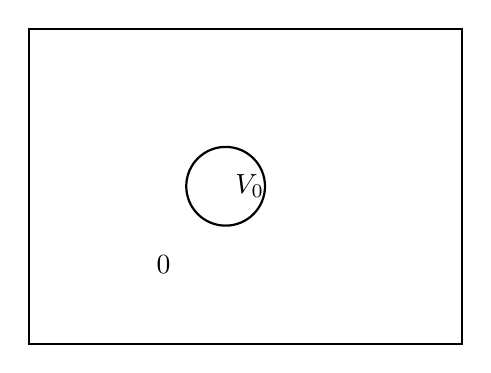
\begin{tikzpicture}
			\draw [-,thick] (0,0) circle (0.5);
			\draw[thick] (-2.5,-2) rectangle (3,2);
			\draw (0,0) node[anchor=west]{$V_0$};
			\draw (-1,-1) node[anchor=west]{$0$};
		\end{tikzpicture}
		\end{figure}
		这是第一类边值问题,$\varphi|_S$已知,上半空间$\rho(\b{r})=0$对应上半空间的格林函数。场点坐标和源点坐标分别可以写为
		\[\b{r}=\begin{pmatrix} R\cos\phi& R\sin\phi &z\end{pmatrix},\quad \b{r}'= \begin{pmatrix} R'\cos\phi' & R'\sin\phi' & z'\end{pmatrix},\]
		第一类边值问题的格林函数可以写为
		\begin{multline*}
			G(\b{r},\b{r}')=\k \left[\frac{1}{\sqrt{R^2+R'^2-2RR'\cos(\phi-\phi')+z^+z'^2-2zz'}}\right. \\ -\left.\frac{1}{\sqrt{R^2+R'^2-2RR'\cos(\phi-\phi')+z^+z'^2+2zz'}}\right],
		\end{multline*}
		计算格林函数在边界上的法向导数
		\[\frac{\partial G}{\partial n'}=-\k\frac{2z}{[R^2+R'^2+z^2-2RR'\cos(\phi-\phi')]^{\frac{3}{2}}},\]
		然后利用我们先前得到的公式进行积分
		\[\varphi(\b{r})=\frac{1}{2\pi}\int_0^a R'\d R'\int_0^{2\pi}V_0\frac{z}{[R^2+R'^2+z^2-2RR'\cos(\phi-\phi')]^{\frac{3}{2}}}\d \phi',\]
		然后利用$R^2+z^2 \gg a^2$的条件进行泰勒展开后计算得到级数解
		\[\varphi(\b{r})=\frac{V_0 a^2}{2}\frac{z}{(R^2+z^2)^{\frac{3}{2}}} \left[ 1-\frac{3}{4}\frac{a^2}{R^2+z^2}+\frac{15}{8}\frac{R^2a^2}{(R^2+z^2)^2}+\cdots\right].\]
		
	\end{eg}
	
	\section{分离变量法}
	\subsection{从泊松方程到拉普拉斯方程}
	重复一遍我们面临的问题:
	\[\nabla^2\varphi=-\frac{\rho}{\varepsilon},\quad \varphi|_S \quad or \quad \left.\frac{\partial \varphi}{\partial n}\right|_S\]
	我们知道,非齐次方程的解等于特解与齐次方程通解之和。我们可以找到最简单的库仑解作为特解:
	\[\varphi_c=\kk\int \frac{\rho(\b{r}')}{|\b{r}-\b{r}'|}\d V',\]
	这样,剩下的问题就是求解齐次的拉普拉斯方程
	\[\nabla^2 \phi=0,\quad \phi=\varphi-\varphi_c.\]
	其边界条件也是可以由原问题中给定的边界条件以及特解在边界上的行为而得到。
	
	求解拉普拉斯方程可以在多种坐标系中进行,本节课将讲解直角坐标和球坐标系下的分离变量法。
	
	\subsection{直角坐标系下的分离变量法}
	\[\nabla^2 \phi=\frac{\partial^2 \phi}{\partial x^2}+\frac{\partial^2 \phi}{\partial y^2}+\frac{\partial^2 \phi}{\partial z^2}=0,\]
	令
	\[\phi(\b{r})=X(x)Y(y)Z(z),\]
	则可以分离变量得到如下形式
	\[\frac{1}{X}\frac{\d^2 X}{\d x^2}=-a^2,\quad \frac{1}{Y}\frac{\d^2 Y}{\d y^2}=-b^2,\quad \frac{1}{Z}\frac{\d^2 Z}{\d z^2}=c^2,\quad a^2+b^2=c^2.\]
	可以写出方程特解
	\[\phi_{ps}=\e^{\pm\i ax}\e^{\pm \i by}\e^{\pm \sqrt{a^2+b^2}z},\]
	通解
	\[\phi=\sum_{a,b}A_{a,b}\e^{\pm\i ax}\e^{\pm \i by}\e^{\pm \sqrt{a^2+b^2}z},\]
	各个系数需要由边界条件来确定。
	
	\subsection{球坐标下的分离变量法}
	\begin{align*}
		\nabla^2 \phi&=\frac{1}{r^2}\frac{\partial }{\partial r}\left(r^2\frac{\partial \phi}{\partial r}\right)+\frac{1}{r^2\sin\theta}\frac{\partial }{\partial \theta}\left(\sin\theta\frac{\partial \phi}{\partial \theta}\right)+\frac{1}{r^2\sin^2\theta}\frac{\partial^2\phi}{\partial \varphi^2} \\
		&=\frac{1}{r}\frac{\partial^2}{\partial r^2}(r\phi)+\cdots
	\end{align*}
	分离变量
	\[\phi(\b{r})=\frac{U(r)}{r}P(\theta)Q(\varphi),\]
	则可以得到方程
	\[\frac{1}{Q}\frac{\d^2 Q}{\d \varphi^2}=-m^2,\]
	\[\frac{1}{\sin\theta}\frac{\d }{\d \theta}\left(\sin\theta\frac{\d P}{\d \theta}\right)+\left[l(l+1)-\frac{m^2}{\sin^2\theta}\right]P=0,\]
	\[\frac{\d^2 U}{\d r^2}-\frac{l(l+1)}{r^2}U=0.\]
	这样我们可以的到通解
	\[Q=\e^{\pm\i m \varphi},\quad m=-l,-l+1,\dots,l\]
	\[P=P_{l}^m(\cos\theta),\quad\text{其中$P_{l}^m$为连带勒让德多项式}\]
	\[\frac{U(r)}{r}=Ar^l+Br^{-(l+1)},\quad l=0,1,2,\dots\]
	在数理方法中,连带勒让德函数的定义为以下方程的解
	\[\frac{\d }{\d x}\left[(1-x^2)\frac{\d P}{\d x}\right]+\left[l(l+1)-\frac{m^2}{1-x^2}\right] P=0,\]
	当$m=0$时,称为勒让德方程,其解称为勒让德多项式,前几个函数为
	\[P_0(x)=1,\quad P_1(x)=x,\quad P_2(x)=\frac{1}{2}(3x^2-1),\dots\]
	勒让德多项式
	\[P_l(x)=\frac{1}{2^l l!}\frac{\d^l}{\d x^l}(x^2-1)^l,\]
	这一组函数具有正交性和完备性
	\[\int_{-1}^1 P_{l'}(x)P_l(x)\d x=\frac{2}{2l+1}\delta_{ll'},\]
	\[f(x)=\sum_{l=0}^\infty  C_l P_l(x),\quad C_l=\frac{2l+1}{2}\int_{-1}^1 f(x)P_l(x)\d x.\]
	而在$m\neq0$时,连带勒让德函数可以由勒让德函数表示出来
	\[P_l^m(x)=(-1)^m(x^2-1)^{\frac{m}{2}}\frac{\d^m P_l(x)}{\d x^m},\]
	它们仍然保持正交性
	\[\int_{-1}^1 P_l^m(x)P_k^m(x)\d x=\frac{(l+m)!}{(l-m)!}\frac{2}{2l+1}\delta_{lk}.\]
	
	下面我们来给出证明以上这些性质的证明。首先,使用幂级数解法可以说明勒让德方程的解即为勒让德多项式,我们在此基础上来证明正交性和完备性,以及连带勒让德多项式的相关性质。
	\begin{proof}
		首先证明引理:若$m<n$,则
		\[\left.\frac{\d^m}{\d x^m}(x^2-1)^n\right|_{-1}^1=0.\]
		这是很好说明的,因为上面的式子可以写成
		\[\left.\sum_{k=0}^m \left(\frac{\d^k}{\d x^k}(x+1)^n\right)\cdot\left(\frac{\d^{m-k}}{\d x^{m-k}}(x-1)^n\right)\right|_{-1}^1, \]
		而$k<n,m-k<n$,所以求和中每项在$x=1,-1$的时候均为0。下面使用这个引力来说明正交性:
		\begin{align*}
			2^m2^nm!n!\int_{-1}^1 P_m(x)P_n(x)\d x&=\int_{-1}^1 \left(\frac{\d^m}{\d x^m}(x^2-1)^m\right)\left(\frac{\d^n}{\d x^n}(x^2-1)^n\right)\d x \\
			&=\left.\left(\frac{\d^m }{\d x^m}(x^2-1)^m\right)\cdot\left(\frac{\d^{n-1}}{\d x^{n-1}}(x^2-1)^n\right)\right|_{-1}^1 \\
			&\qquad -\int_{-1}^1 \left(\frac{\d^{m+1} }{\d x^{m+1}}(x^2-1)^m\right)\cdot\left(\frac{\d^{n-1}}{\d x^{n-1}}(x^2-1)^n\right)\d x \\
			&=(-1)^n\int_{-1}^1 (x^2-1)^n\frac{\d^{m+n}}{\d x^{m+n}}(x^2-1)^m \d x
		\end{align*}
		当$m\neq n$时,不妨设$m < n$,则我们会发现在进行分部积分的过程中有一项已经变成了零,所以它们时正交的。而如果$m=n$,那么此时方程就变成了
		\[\int_{-1}^1 P_n(x)P_n(x)\d x=\frac{(2n)!}{2^{2n}n!n!}(-1)^n\int_{-1}^1(x^2-1)^n\d x=\frac{2}{2n+1}.\]
		完备性暂时没找到比较好的证明,不过在假定完备性的基础上叠加系数是可以由正交性算出来的。
		
		应该说明的是勒让德多项式有更自然的引入方法,例如从一系列非线性相关但是又不是互相正交的幂函数$1,x,x^2,\dots$出发,进行施密特正交化,得到的其实就是勒让德多项式。此外,还可以证明勒让德多项式所具有的递推性质。
		
		连带勒让德多项式性质的证明是类似的,这里就不赘述。这一部分详细的内容在数学物理方法书上都能找到。
	\end{proof}
	
	\subsection{球谐函数}
	定义角动量算符
	\[\hat{L}^2=\frac{1}{\sin\theta}\frac{\partial }{\partial \theta}\left(\sin\theta\frac{\partial }{\partial \theta}\right)+\frac{1}{\sin^2\theta}\frac{\partial^2}{\partial \varphi^2},\]
	则拉普拉斯方程可以写为
	\[\nabla^2\phi=\frac{1}{r^2}\frac{\partial }{\partial r}\left(r^2\frac{\partial \phi}{\partial r}\right)-\frac{\hat{L}^2}{r^2},\]
	之前的分离变量可以写为这种形式
	\[\hat{L}^2 Y_{lm}(\theta,\varphi)=l(l+1)Y_{lm}(\theta,\varphi),\]
	其中
	\[Y_{lm}(\theta,\varphi)=\sqrt{\frac{(2l+1)}{4\pi}\frac{(l-m)!}{(l+m)!}}P_l^m(\cos\theta)\e^{\i m\varphi},\]
	这称为球谐函数。可以写出常用的几项
	\[Y_{00}=\frac{1}{\sqrt{4\pi}},\quad Y_{10}=\sqrt{\frac{3}{4\pi}}\cos\theta,\quad Y_{11}=-\sqrt{\frac{3}{8\pi}}\sin\theta\e^{\i \varphi},\quad Y_{1,-1}=-\sqrt{\frac{3}{8\pi}}\sin\theta\e^{-\i \varphi}.\]
	球谐函数仍然是正交归一的,利用三维空间中的单位矢量可以写成
	\[Y_{lm}(\theta,\varphi)=Y_{lm}(\hat{\b{n}}),\quad Y_{l,-m}(\hat{\b{n}})=(-1)^m Y_{lm}^*(\hat{\b{n}}),\]
	\[\int Y_{lm}^*(\hat{\b{n}})Y_{l'm'}(\hat{\b{n}})\d \Omega_{\hat{\b{n}}}=\delta_{ll'}\delta{mm'},\]
	完备性
	\[\sum_{l=0}^\infty \sum_{m=-l}^l Y_{lm}^*(\hat{\b{n}}')Y_{lm}(\hat{\b{n}})=\delta(\cos\theta'-\cos\theta)\delta(\varphi'-\varphi),\]
	有了这两个性质之后,我们可以将拉普拉斯方程的解用球谐函数展开
	\[\phi(r,\theta,\varphi)=\sum_{l=0}^\infty\sum_{m=-l}^l \left(A_{lm}r^l+\frac{B_{lm}}{r^{l+1}}\right)Y_{lm}(\theta,\varphi),\]
	叠加系数由边界条件确定下来。
	
	\begin{eg}
		无穷大均匀介质有一$z$方向的均匀电场$\b{E}_0=E\hat{\b{e}}_z$,在介质中挖去一半径为$R$的球形空穴,求变化后的电场。
		\begin{figure}[H]
			\centering
			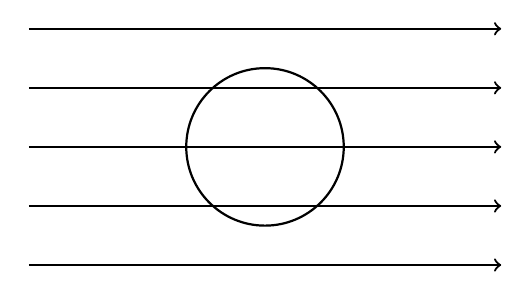
\begin{tikzpicture}
				\draw[thick] (0,0)circle(1);
				\draw[->,thick] (-3,0)--(3,0);
				\draw[->,thick] (-3,0.75)--(3,0.75);
				\draw[->,thick] (-3,1.5)--(3,1.5);
				\draw[->,thick] (-3,-0.75)--(3,-0.75);
				\draw[->,thick] (-3,-1.5)--(3,-1.5);
			\end{tikzpicture}
		\end{figure}
		注意,在求解问题前应先观察问题的对称性,从而决定使用哪种方法。本题中问题具有某种球形对称,因此使用球坐标下的分离变量法。
		
		先将问题用数学语言表述出来
		\[\left\{\begin{gathered}
			\nabla^2 \varphi_1=0, \quad r>R\\ 
			\nabla^2 \varphi_2 =0,\quad r<R\end{gathered}\right.,\quad \varphi_1|_{r=R}=\varphi_2|_{r=R},\quad \varepsilon_1\left.\frac{\partial \varphi_1}{\partial r}\right|_{r=R}=\varepsilon_2\left.\frac{\partial \varphi_2}{\partial r}\right|_{r=R},\]
		在无穷远处应该有
		\[\nabla\varphi|_\infty=-b{E}_0\Rightarrow \varphi_1|_\infty=-E_0z.\]
		同时还可以注意到,问题是关于$\varphi$对称的,所以解是与$\varphi$无关的,因此可以取$m=0$,所以解可以写成
		\[\left\{\begin{gathered}
			\varphi_1=\sum_{l} \left[A_l r^l+B_lr^{-(l+1)}\right]P_l(\cos\theta),\quad r>R, \\
			\varphi_2=\sum_{l} \left[C_l r^l+D_lr^{-(l+1)}\right]P_l(\cos\theta),\quad r<R,
		\end{gathered}\right.\]
		下面要做的就是用边界条件和连接条件来确定四组系数。先考虑无穷远处的条件,我们可以知道$A_1\neq0$,因此可以写成
		\[\varphi_1=-E_0r\cos\theta+\sum_{l}B_lr^{-(l+1)}P_l(\cos\theta),\]
		另外由于在$r=0$处无电荷,因此电势应该有限,所以
		\[\varphi_2=\sum_l C_l r^lP_l(\cos\theta).\]
		接下来考虑$r=R$处,由于$\varphi_1=\varphi_2$,因此应该有
		\[-E_0 R\cos\theta+\sum_{l} B_lR^{-(l+1)}P_l(\cos\theta)=\sum_lC_lR^lP_l(\cos\theta),\]
		由$\varepsilon_1\left.\frac{\partial \varphi_1}{\partial r}\right|_{r=R}=\varepsilon_2\left.\frac{\partial \varphi_2}{\partial r}\right|_{r=R}$有
		\[-\varepsilon_1E_0\cos\theta-\sum_l \varepsilon_1 (l+1)R^{-(l+2)}P_l(\cos\theta)=\sum_l\varepsilon_2lC_lR^{l-1}P_l(\cos\theta),\]
		联立之后,利用正交完备性,就可得到最终的解
		\[\varphi_1=-E_0z+\frac{B_1\cos\theta}{r^2},\quad \varphi_2=C_1z,\]
		这给出球内的电场
		\[\b{E}_2=C_1\hat{\b{e}}_z.\]
	\end{eg}
	
	\subsection{柱坐标下的分离变量法}
	尽管我们在静电场问题中遇到的大量问题都是用球坐标求解的(或许是出题人奇怪的癖好吗),但是柱坐标下的分离变量法也是比较重要的。考虑在柱坐标下求解拉普拉斯方程,我们假设问题与$z$无关,那么方程就可以写成
	\[\frac{1}{\rho}\frac{\partial u}{\partial \rho}\left(\rho\frac{\partial u}{\partial \rho}\right)+\frac{1}{\rho^2}\frac{\partial^2 u}{\partial \phi^2}=0,\]
	分立变量
	\[u(\rho,\phi)=R(\rho)\varphi(\phi),\]
	于是有
	\[\left\{\begin{aligned}
		\rho\frac{\d }{\d \rho}\left(\rho\frac{\d R}{\d \rho}\right)&=\lambda R, \\
		\frac{\d^2\varphi}{\d \phi^2}&=-\lambda\varphi.
	\end{aligned}\right.\]
	第二个方程的通解是很好写出的
	\[\varphi(\phi)=C\sin\sqrt{\lambda}\phi+D\cos\sqrt{\lambda}\phi,\]
	第一个方程不太容易直接看出,我们引入参变量$s=\ln \rho$,于是
	\[\frac{\d }{\d \rho}=\frac{\d s}{\d \rho}\frac{\d }{\d s}=\frac{1}{\rho}\frac{\d }{\d s},\]
	因此第一个方程就可以写为
	\[\frac{\d^2  R}{\d s^2}=\lambda R, \]
	由此就可以写出通解
	\[R(\rho)=Ar^{\sqrt{\lambda}}+Br^{-\sqrt{\lambda}}.\]
	
	\chapter{静磁场}
	磁场与电场的根本区别在于其源的最小单位为磁偶极子,没有单一的磁荷。人们最早接触到的铁磁现象是比较复杂的,我们先研究电流产生的磁场。
	\section{磁场的矢势及微分方程}
	静磁场满足微分方程
	\[\nabla\cdot\b{B}=0,\quad \nabla\times\b{H}=\b{j}_f.\]
	守恒律对应着
	\[\nabla\cdot\b{j}_f.\]
	对于线性介质,有
	\[\b{B}=\mu \b{H},\]
	于是第二个方程就可以写成
	\[\nabla\times\b{B}=\mu\b{j}_f.\]
	\subsection{磁场的矢势}
	引入矢势$\b{A}$,使得
	\[\b{B}=\nabla\times\b{A},\]
	这样静电场的第一个方程就自动满足了。对于第一个方程,考虑对其作曲面积分,对于两个由同一个环路围城的曲面,由高斯公式
	\[\int_{S_1}\b{B}\cdot\d \b{S}-\int_{S_2}\b{B}\cdot\d\b{S}=\int_V \nabla\cdot\b{B}\d V=0.\]
	同时,
	\[\int_{S_1}\b{B}\cdot\d\b{S}=\int_{S_1}(\nabla\times\b{A})\cdot\d\b{S}=\oint_{l}\b{A}\cdot\d\b{l}.\]
	这说明静磁场矢势的环路积分是唯一的。
	
	矢势的规范变换我们在先前已经涉及了,这里不再赘述。以下我们选取库仑规范$\nabla\cdot\b{A}=0$进行讨论。
	
	注:库仑规范的完整形式在电磁波那一章中给出,这里用了静电场的条件。
	
	\subsection{矢势的微分方程}
	由静磁场满足的方程,将矢势定义带入就得到
	\[\mu\b{j}_f=\nabla\times(\nabla\times\b{A})=\nabla(\nabla\cdot\b{A})-\nabla^2\b{A}=-\nabla^2\b{A}.\]
	这称为磁矢势所满足的泊松方程。
	
	\subsection{磁矢势的库仑解}
	对照静电学中的库仑解,我们可以得到静磁学中的库仑解
	\[\b{A}(\b{r})=\frac{\mu}{4\pi}\int \frac{\b{j}(\b{r}')\d V'}{|\b{r}-\b{r}'|},\]
	计算对应的磁感应强度
	\begin{align*}
		\b{B}(\b{r})&=\nabla\times\b{A}(\b{r})\\
		&=\nabla\times\frac{\mu}{4\pi}\int \frac{\b{j}(\b{r}')\d V'}{|\b{r}-\b{r}'|} \\
		&=\frac{\mu}{4\pi}\int\left(\nabla\frac{1}{|\b{r}-\b{r}'|}\right)\times\b{j}(\b{r}')\d V' \\
		&=\frac{\mu}{4\pi}\int \frac{\b{j}(\b{r}')\times(\b{r}-\b{r}')}{|\b{r}-\b{r}'|^3}\d V'
	\end{align*}
	这就是我们在实验中得到的毕奥-萨伐尔定律。
	
	\subsection{边值关系}
	静磁场满足边值关系
	\[\hat{\b{e}}_n\cdot(\b{B}_2-\b{B}_1)=0,\quad \hat{\b{e}}_n\times(\b{H}_2-\b{H}_1)=\b{\alpha}.\]
	考虑到线性介质,将矢势带入得到矢势满足的边值关系
	\[\hat{\b{e}}_n\cdot(\nabla\times\b{A}_2-\nabla\times\b{A}_1)=0,\]
	\[\hat{\b{e}}_n\times\left(\frac{1}{\mu_2}\nabla\times\b{A}_2-\frac{1}{\mu_1}\nabla\times\b{A}_1\right)=\b{\alpha}.\]
	这两个方程都不太简单,我们通过常用的在界面上取微元的方法可以得到第一个式子的替代形式
	下面考虑库仑规范,在介质交界面处取一个垂直于界面的小圆柱,由高斯公式
	\[\oint \b{A}\cdot\d \b{S}=\int \nabla\cdot\b{A} \d V=0,\]
	圆柱侧面可以趋向于无穷小,因此可以得到两边的矢势法向分量是相等的
	\[A_{1n}=A_{2n}.\]
	再在交界面取一个围成的面积无穷小但具有有限长度的闭合回路,则
	\[\oint \b{A}\cdot\d\b{l}=\int \b{B}\cdot\d\b{S}=0,\]
	故
	\[\b{A}_{1t}=\b{A}_{2t}.\]
	综合以上两项,就得到静磁场磁矢势所满足的边值关系
	\[\b{A}_1=\b{A}_2.\]
	应当注意,这个关系只能够取代上面的第一个边值关系,而并不能取代有关磁场强度的那个边值关系。
	
	理论上,由相应的泊松方程及边值条件,我们可以得到任何问题的解。
	
	\section{磁矢势法}
	这里给出几个用磁矢势法来计算磁场分布的例子。
	\subsection{无穷长直线}
	\begin{figure}[H]
		\centering
	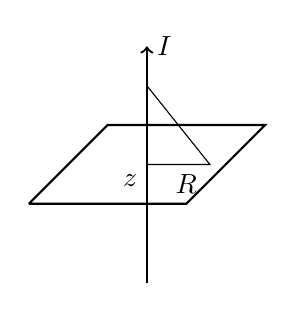
\begin{tikzpicture}
		\draw [thick](0,0)--(1,1)--(3,1)--(2,0)--(0,0);
		\draw [->,thick](1.5,-1)--(1.5,2) node[anchor=west]{$I$};
		\draw (1.5,0.5)--(2.3,0.5)--(1.5,1.5);
		\draw (2,0.5) node[anchor=north]{$R$};
		\draw (1.5,0.3) node[anchor=east]{$z$};
		
	\end{tikzpicture}
	\end{figure}
	\[\b{A}(\b{r})=\frac{\mu}{4\pi}\int \frac{\b{j}(\b{r}')}{|\b{r}-\b{r}'|}\d V' = \frac{\mu}{4\pi}\int \frac{I}{|\b{r}-\b{r}'|}\d \b{l}'.\]
	由于这个积分是发散的,因此我们取$R_0$处矢势为零,于是
	\[\b{A}=-\frac{\mu_0 I}{2\pi}\ln\frac{R}{R_0}\hat{\b{e}}_z.\]
	于是
	\[\b{B}=\nabla\times\b{A}=-\frac{\mu_0 I}{2\pi}\frac{1}{R}\hat{\b{e}}_R\times\hat{\b{e}}_z=\frac{\mu_0 I}{2\pi}\frac{1}{R}\hat{\b{e}}_\phi.\]
	
	\subsection{环形电流}
	采用球坐标进行计算,电流分布可以写成
	\begin{figure}[H]
		\centering
		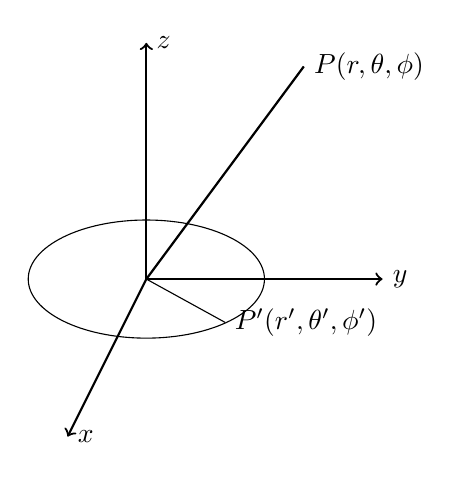
\begin{tikzpicture}
			\draw [->,thick](0,0)--(-1,-2) node [anchor=west]{$x$};
			\draw [->,thick](0,0)--(3,0) node [anchor=west]{$y$};
			\draw [->,thick](0,0)--(0,3) node [anchor=west]{$z$};
			\draw (0,0) ellipse (1.5 and 0.75);
			\draw [thick](0,0)--(2,2.7) node[anchor=west]{$P(r,\theta,\phi)$};
			\draw (0,0)--(1,-0.55) node[anchor=west]{$P'(r',\theta',\phi')$};
		\end{tikzpicture}
	\end{figure}
	\[\b{j}(\b{r}')=c\delta(r'-a)\delta(\theta'-\frac{\pi}{2})\hat{\b{e}}_\phi.\]
	于是
	\[\b{A}(\b{r})=\frac{\mu}{4\pi}\oint \frac{I\d\b{l}'}{|\b{r}-\b{r}'|}=\frac{\mu I a}{4\pi}\int_0^{2\pi}\frac{\hat{\b{e}}_{\phi'}\d\phi'}{|\b{r}-a\hat{\b{e}}_{r'}|}.\]
	进行对称性分析(从垂直于$x-y$平面的方向上去看),可以得到,最终的矢势可以写成这样的形式
	\[\b{A}(\b{r})=A_\phi\hat{\b{e}}_\phi.\]
	于是
	\[A_\phi=\frac{\mu I a}{4\pi}\int_0^{2\pi}\frac{\hat{\b{e}}_\phi\cdot\hat{\b{e}}_{\phi'}\d\phi'}{|\b{r}-a\hat{\b{e}}_{r'}|}.\]
	由于对称性,我们考虑$\phi=0$,此时
	\[\hat{\b{e}}_\phi\cdot\hat{\b{e}}_{\phi'}=\cos\phi',\quad|\b{r}-a\hat{\b{e}}_{r'}|=(r^2+a^2-2ra\sin\theta\cos\phi')^{1/2}. \]
	于是
	\[A_\phi=\frac{\mu Ia}{4\pi}\int_0^{2\pi}\frac{\cos\phi'\d \phi'}{\sqrt{r^2+a^2-2ra\sin\theta\cos\phi'}}.\]
	下面考虑$r\gg a$的情况,则
	\[\frac{1}{\sqrt{r^2+a^2-2ra\sin\theta\cos\phi'}}\approx \frac{1}{r}+\frac{a\sin\theta\cos\phi'}{r^2},\]
	进行积分就得到
	\[A_\phi=\frac{\mu Ia^2}{4}\frac{\sin\theta}{r^2}.\]
	定义
	\[\b{m}=I\pi a^2\hat{\b{e}}_z,\]
	则
	\[\b{A}=\frac{\mu}{4\pi}\frac{\b{m}\times\b{r}}{r^3}.\]
	计算磁感应强度
	\begin{align*}
		\b{B}&=\frac{\mu}{4\pi}\nabla\times\left(\b{m}\times\frac{\b{r}}{r^2}\right) \\
		&=\frac{\mu}{4\pi}\left[\b{m}\left(\nabla\cdot\frac{\b{r}}{r^3}\right)-(\b{m}\cdot\nabla)\frac{\b{r}}{r^3}\right].
	\end{align*}
	(回忆一下这里用的这个矢量运算公式,其实应该有四项,但是为$\b{m}$(对于$\b{r}$)是一个常量,所以只剩下了两项。)
	
	由于
	\[\nabla\cdot\left(\frac{\b{r}}{r^3}\right)=4\pi\delta(\b{r}),\]
		\[\nabla\times\left(\frac{\b{r}}{r^3}\right)=0,\]
	在远场$r\neq0$,所以
	\begin{align*}
		\b{B}(\b{r})&=-\frac{\mu}{4\pi}(\b{m}\cdot\nabla)\frac{\b{r}}{r^3} \\
		&=-\frac{\mu}{4\pi}\nabla\left(\frac{\b{m}\cdot\b{r}}{r^3}\right),
	\end{align*}
	这样,我们引入了磁标势
	\[\varphi_m=\frac{1}{4\pi}\frac{\b{m}\cdot\b{r}}{r^3},\quad \b{B}=-\mu\nabla\varphi_m(\b{r}),\]
	\[\b{B}(\b{r})=\frac{\mu}{4\pi}\frac{3\b{m}\cdot\hat{\b{e}}_r\hat{\b{e}}_r-\b{m}}{r^3},\]
	这个式子称为磁偶极场,相应的,$\b{m}$称为磁偶极矩,这个概念非常重要,在这里只是作为一个例子引入,之后会有严格的推导。
	
	\section{静磁场的多极展开}
	静磁学多极展开的思想与静电学多极展开的思想是非常类似的,即对于一个小区域内的源,考虑其在远处的场。
	\subsection{磁矢势的多极展开法}
	磁场情形中,我们只考虑前两项展开
	\[\frac{1}{|\b{r}-\b{r}'|}=\frac{1}{r}-\b{r}'\cdot\nabla\frac{1}{r}+\cdots=\frac{1}{r}+\frac{\b{r}'\cdot\hat{\b{e}}_r}{r^2}+\cdots,\]
	\[\b{A}(\b{r})=\b{A}_0+\b{A}_1+\cdots\]
	\[\b{A}_0(\b{r})=\frac{\mu}{4\pi}\frac{1}{r}\int \b{j}(\b{r}')\d V',\]
	\[\b{A}_1(\b{r})=\frac{\mu}{4\pi}\frac{\b{r}}{r^3}\cdot\int \b{r}'\b{j}(\b{r}')\d V'.\]
	
	\subsection{磁矢势}
	先考虑磁零极矩$\b{A}_0$,由于电流场稳恒,因此可以将电流看作许多闭合流管,考虑其中的一个流管,应该有
	\[\int \b{j}(\b{r}')\d V'=I\oint\d \b{l}=0.\]
	这说明
	\[\b{A}_0(\b{r})=0,\]
	即磁单极不存在。这是合理的。
	
	再来考虑磁偶极矩,我们先证如下三重并矢的散度公式
	\[\nabla\cdot(\b{j}\b{r}\b{r})=\b{j}\b{r}+\b{r}\b{j}.\]
	\begin{proof}
		\begin{align*}
			\nabla\cdot(\b{j}\b{r}\b{r}) &= \nabla\cdot(j_i\hat{\b{e}}_ix_j\hat{\b{e}}_jx_k\hat{\b{e}}_k) \\
			&=\partial_i(j_ix_jx_k)\hat{\b{e}}_j\hat{\b{e}}_k \\
			&=(x_jx_k\partial_i j_i+j_ix_jx_k\delta_{ij}+j_ix_jx_k\delta_{ik})\hat{\b{e}}_j\hat{\b{e}}_k\\
			&=(\nabla\cdot\b{j})\b{r}\b{r}+\b{j}\b{r}+\b{r}\b{j}.
		\end{align*}
		考虑稳恒条件下的连续性方程,第一项为零,因此就得到结论。
	\end{proof}
	由我们使用多极展开的前提,即考虑的空间远大于有源空间,因此有
	\[\int \nabla'\cdot(\b{j}\b{r}'\b{r}')\d V'=\oint \b{j}\b{r}'\b{r}'\cdot\d S'=0,\]
	所以
	\[\int\b{j}(\b{r}')\b{r}'\d V'=-\int\b{r}'\b{j}(\b{r}')\d V'.\]
	所以
	\begin{align*}
		\hat{\b{e}}_r\cdot\int\b{r}'\b{j}(\b{r}')\d V'&=-\frac{1}{2}\int \hat{\b{e}}_r\cdot(\b{j}(\b{r}')\b{r}'-\b{r}'\b{j}(\b{r}'))\d V' \\
		&=-\frac{1}{2}\int \hat{\b{e}}_r\times(\b{r}'\times\b{j}(\b{r}'))\d V'
	\end{align*}
	这样,就可以写出第二项
	\[\b{A}_1(\b{r})=-\frac{\mu}{4\pi}\frac{1}{2r^2}\hat{\b{e}}_r\times\int (\b{r}'\times\b{j}(\b{r}'))\d V' = \frac{\mu}{4\pi}\frac{\b{m}\times\hat{\b{e}}_r}{r^2},\]
	其中
	\[\b{m}=\frac{1}{2}\int (\b{r}'\times\b{j}(\b{r}'))\d V'\]
	这就是针对一般电流分布定义的磁偶极矩。
	
	\subsection{球坐标下磁矢势的多极展开}
	回忆在静电场情形中球坐标下的多极展开,有关系
	\[\frac{1}{|\b{r}-\b{r}'|}=\sum_{l=0}^\infty \frac{r'^l}{r^{l+1}}P_l(\cos\gamma),\]
	代入磁矢势表达式中就有
	\[\b{A}(\b{r})=\frac{4\pi r}{\mu}\int \sum_{l=0}^\infty \left(\frac{r'}{r}\right)^lP_l(\cos\gamma)\b{j}(\b{r}')\d V',\]
	保留前两项,
	\[\b{A}(\b{r})=\frac{\mu}{4\pi r}\int \b{j}(\b{r}')\d V' + \frac{\mu}{4\pi r}\int \frac{r'}{r}\cos\gamma\b{j}(\b{r}')\d V' + \cdots\]
	注意到,这里的第一项即为直角坐标系中的多极展开的$\b{A}_0$,故
	\[\b{A}(\b{r})=\b{A}_1(\b{r})=\frac{\mu}{4\pi r^2}\int \hat{\b{e}}_r \cdot\b{r}'\b{j}(\b{r}')\d V'+\cdots\]
	这与先前得到的结果也是相同的。
	
	\subsection{磁偶极子的磁场}
	由上面的讨论我们得出,在原场条件下,我们只要考虑磁偶极子产生的磁场
	\[\b{A}(\b{r})\approx\b{A}_1(\b{r})=\frac{\mu}{4\pi}\frac{\b{m}\times\hat{\b{e}}_r}{r^2},\]
	计算磁感应强度
	\begin{align*}
		\b{B}_1&=\nabla\times\b{A}_1=\frac{\mu}{4\pi}\nabla\times(\b{m}\times\frac{\b{r}}{r^3}) \\
		&=\frac{\mu}{4\pi}\left[\left(\nabla\cdot\frac{\b{r}}{r^3}\right)\b{m}-(\b{m}\cdot\nabla)\frac{\b{r}}{r^3}\right] \\
		&=-\frac{\mu}{4\pi}(\b{m}\cdot\nabla)\frac{\b{r}}{r^3}\\
		&=-\frac{\mu}{4\pi}(\b{m}\cdot\nabla)\frac{\b{r}}{r^3}-\frac{\mu}{4\pi}\b{m}\times\left(\nabla\times\frac{\b{r}}{r^3}\right) \\
		&=-\frac{\mu}{4\pi}\nabla\left(\frac{\b{m}\cdot\b{r}}{r^3}\right) \\
		&=-\mu\nabla\varphi_m.
	\end{align*}
	这个推导其实在多极展开之前已经进行过了, 这里稍微写的详细了一点,对于矢量运算要非常熟悉才能顺利地进行推导。
	
	\subsection{局域电流分布在外磁场中的能量}
	分成几种情况来讨论
	\subsubsection{真空只有静磁场}
	磁场的总能量
	\[W=\frac{1}{2}\int \b{B}\cdot\b{H}\d V=\frac{1}{2\mu_0}\int B^2 \d V,\]
	而利用磁矢势我们可以这样推导
	\[\b{B}\cdot\b{H}=(\nabla\times\b{A})\cdot\b{H}=\nabla\cdot(\b{A}\times\b{H})+\b{A}\cdot(\nabla\times\b{H})=\nabla\cdot(\b{A}\times\b{H})+\b{A}\cdot\b{j},\]
	于是
	\[W=\frac{1}{2}\int \b{A}\cdot\b{j}\d V.\]
	第一项积分化为了无穷远处界面上的积分,从而是趋于零的。这就再一次提醒我们,上述的计算是对于全空间的总能量进行的,如果要计算某个局域部分的能量,则不能这么处理。
	
	\subsubsection{电流分布与外磁场相互作用能}
	将电流$\b{j}$置于由外源$\b{j}_e$激发的电磁场中,相互作用能
	\begin{align*}
		W_{int}&=\frac{1}{2}\int (\b{j}+\b{j}_e)\cdot(\b{A}+\b{A}_e)\d V - \frac{1}{2}\int\b{j}\cdot\b{A}\d V - \frac{1}{2}\int \b{j}_e\cdot\b{A}_e\d V \\
		&=\frac{1}{2}\int (\b{j}\cdot\b{A}_e+\b{A}\cdot\b{j}_e)\d V \\
		&=\int \b{j}\cdot\b{A}_e \d V.
	\end{align*}
	最后一步用到了两个积分相同,可以这样证明:
	\[\b{A}(\b{r})=\frac{\mu_0}{4\pi}\int \frac{\b{j}(\b{r}')}{|\b{r}-\b{r}'|}\d V',\quad \b{A}_e(\b{r})=\frac{\mu_0}{4\pi}\int \frac{\b{j}_e(\b{r}'')}{|\b{r}-\b{r}''|}\d V''\]
	于是
	\[\int \b{A}_e(\b{r})\cdot\b{j}(\b{r})\d V=\frac{\mu_0}{4\pi}\int \d V\d V''\frac{\b{j}_e(\b{r}'')\cdot\b{j}(\b{r})}{|\b{r}-\b{r}'|}=\int \b{A}(\b{r})\cdot\b{j}_e(\b{r})\d V.\]
	
	\subsubsection{局域电流分布——磁偶极子在外磁场中能量}
	改写相互作用能部分,考虑一个电流流管,
	\[W_{int}=\int \b{A}_e\cdot\b{j}\d V = I\oint \b{A}_e\cdot\d \b{l}'= I \int_s(\nabla\times\b{A}_e)\cdot\d \b{S}' = I\int_s\b{B}_e\cdot\d \b{S}',\]
	取电流分布中任一点o为原点,则对于很小范围内的$\b{r}$
	\[\b{B}_e(\b{r})=\b{B}_e(0)+\b{r}\cdot\nabla\b{B}_e(0),\]
	在这样的假设下,电流管实际上已经成为了磁偶极子模型。引入磁偶极矩$\b{m}$之后,它在外场中的能量就写成
	\[W_{int}=I\int\d \b{S}'\cdot\b{B}_e(0)=\b{m}\cdot\b{B}_e(0).\]
	
	\subsubsection{磁偶极子在外场中受力}
	小区域内电流$\b{j}(\b{r})$在外磁场$\b{B}_e$中受力
	\[\b{F}=\int \b{j}(\b{r})\times\b{B}_e\d V,\]
	利用上面用过的选取原点后磁感应强度的表达式,有
	\[\b{F}=\int \b{j}(\b{r})\times\b{B}_e(0)\d V + \int\b{j}(\b{r})\times\left[\b{r}\cdot\nabla\b{B}_e(0)\right]\d V=\nabla W_{int}.\]
	第一项为零因此
	\begin{align*}
		\b{F}&=\int \left[\b{j}(\b{r})\b{r}\cdot\nabla\right]\times\b{B}_e(0)\d V \\
		&=\frac{1}{2}\int \d V(\b{j}\b{r}-\b{r}\b{j})\cdot\nabla\times\b{B}_e \\
		&=\frac{1}{2}\int \d V\left[(\b{r}\times\b{j})\times\nabla\right]\times\b{B}_e \\
		&=\b{m}\times\nabla\times\b{B}_e(0) \\
		&=\nabla(\b{m}\cdot\b{B}_e(0)).
	\end{align*}
	力矩
	\begin{align*}
		\b{N}_B&=\int \b{r}\times\b{f}(\b{r})\d V = \int\b{r}\times(\b{j}(\b{r})\times\b{B}(\b{r}))\d V\\ 
		&=\int \b{r}\times(\b{j}(\b{r})\times\b{B}(0))\d V \\
		&= \b{m}\times\b{B}_e(0)
	\end{align*}
	
	\section{磁标势法}
	\subsection{磁标势的引入}
	从前面的讨论中我们已经知道,磁荷不存在,且磁场有旋,因此我们一般不引入标势来描述磁场。但若处理空间无自由电流分布的问题,此时
	\[\nabla\times\b{H}=0,\]
	此时我们可以仿照静电学引入磁标势
	\[\b{H}(\b{r})=-\nabla\varphi_m(\b{r}).\]
	这两个边界条件前者对应$\b{H}$切向连续,后者对应$\b{B}$法向连续,因此在实际计算时,直接这样可以选择更为方便的来使用(尤其是第二个法向导数的条件,对于更一般的极化情况,还是使用$\hat{\b{e}}_n\cdot(\b{B}_2-\b{B}_1)$更方便。)
	
	\subsection{非铁磁线性介质}
	非铁磁线性介质满足这样简单的关系
	\[\b{B}=\mu\b{H},\]
	无自由电流时,引入磁标势
	\[\b{H}=-\nabla\varphi_m,\]
	\[\nabla\cdot\b{B}=0 \quad \Rightarrow \quad \nabla^2\varphi_m(\b{r})=0,\]
	这是标准的拉普拉斯方程,因此也有相应的边值条件
	\[\varphi_{m1}=\varphi_{m2},\quad \mu_1\frac{\partial \varphi_{m1}}{\partial n}=\mu_2\frac{\partial \varphi_{m2}}{\partial n}.\]
	
	\subsection{永久铁磁的磁标势方程}
	\[\nabla\times\b{H}=0,\quad \nabla\cdot\b{B}=0,\quad \b{B}=\mu_0(\b{H}+\b{M}),\]
	与静电场$\nabla\cdot\b{P}=-\rho_f$相对应的,引入假想磁荷分布
	\[\rho_m=-\mu_0\nabla\cdot\b{M},\]
	这样可以得到
	\[\nabla^2\varphi_m = -\frac{\rho_m}{\mu_0},\]
	这是一个标准的泊松方程,此时边界条件改为
	\[\varphi_{m1}=\varphi_{m2},\quad \frac{\partial \varphi_{m2}}{\partial n}-\frac{\partial \varphi_{m1}}{\partial n}=\hat{\b{e}}_n\cdot(\b{M}_2-\b{M}_1).\]
	
	\subsection{磁标势公式与静电势公式对比}
	\begin{table}[H]
		\centering
		\begin{tabular}{c|c}
			\hline
			静电场 & 静磁场(无自由电流) \\ \hline
			$\nabla \times \b{E}=0$ & $\nabla\times\b{H}=0$ \\ \hline
			$\nabla\cdot\b{E}=(\rho_f+\rho_p)/\varepsilon_0
			$ & $\nabla\cdot\b{H}=\rho_m/\mu_0$ \\ \hline
			$\rho_p=-\nabla\cdot\b{P}$ & $ \rho_m=-\mu_0\nabla\cdot\b{M}$ \\ \hline
			$ \b{D}=\varepsilon_0\b{E}+\b{P}$ & $\b{B}=\mu_0\b{H}+\mu_0\b{M}$\\ \hline 
			$ \b{E}=-\nabla\varphi$ & $\b{H}=-\nabla\varphi_m$ \\ \hline
			$ \nabla^2\varphi=-(\rho_f+\rho_p)/\varepsilon_0$ & $\nabla^2\varphi_m=-\rho_m/\mu_0$ \\ \hline 
		\end{tabular}
	\end{table}
	
	\subsection{例题}
	\begin{eg}
		有一匀强磁化的铁磁球,半径为$a$,磁化强度为$M$,求它产生的磁场。
		
		\begin{figure}[H]
			\centering
		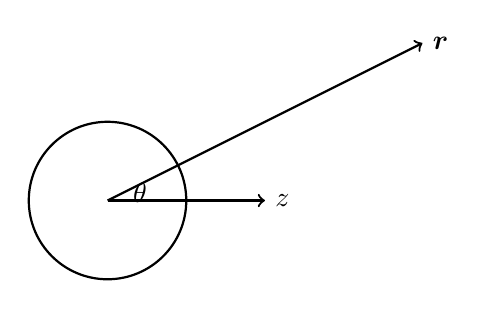
\begin{tikzpicture}
			\draw [thick] (0,0)ellipse (1 and 1);
			\draw [->,thick] (0,0)--(2,0)node [anchor=west]{$z$};
			\draw [->,thick] (0,0)--(4,2)node [anchor=west]{$\b{r}$};
			\draw (0.2,0.1)node[anchor=west]{$\theta$};
		\end{tikzpicture}
		\end{figure}
		将磁标势分成内外两部分来考虑,
		\[\nabla^2\varphi_{in}=0,\quad \nabla^2\varphi_{out}=0,\]
		\[\rho_m=-\mu_0\nabla\cdot\b{M}=0,\]
		连接条件
		\[\varphi_{in}|_{r=a}=\varphi_{out}|_{r=a},\quad -\left.\frac{\partial \varphi_{in}}{\partial r}\right|_{r=a}+M\cos\theta=-\left.\frac{\partial \varphi_{out}}{\partial r}\right|_{r=a},\]
		又因为物理要求
		\[\varphi_{out}|_{r\rightarrow \infty}=0,\quad \varphi_{in}|_{r=0}\text{有限},\]
		因此内外的解可以分别写为
		\[\varphi_{out}=\sum_{l=0}^\infty \frac{b_l}{r^{l+1}}P_l(\cos\theta),\quad \varphi_{in}=\sum_{l=0}^\infty a_lr^lP_l(\cos\theta).\]
		再考虑连接条件,就可以得到叠加系数,于是
		\[\varphi_{in}=\frac{1}{3}Mr\cos\theta,\quad \varphi_{out}=\frac{Ma^2}{3r^2}\cos\theta=\frac{1}{4\pi}\frac{\b{m}\cdot\b{r}}{r^3},\quad \b{m}=\frac{4\pi}{3}a^3\b{M}.\]
		球内磁场
		\[\b{H}_{in}=-\frac{1}{3}\b{M},\]
		球外磁场
		\[\b{B}_{out}=\frac{\mu_0}{4\pi}\frac{3\b{m}\cdot\hat{\b{e}}_r\hat{\b{e}}_r-\b{m}}{r^3}.\]
		
	\end{eg}
	
	\begin{eg}
		磁屏蔽
		\begin{figure}[H]
			\centering
			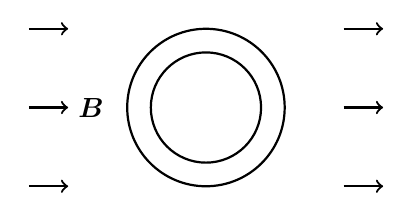
\begin{tikzpicture}
				\draw [->,thick](0,0)--(0.5,0)node[anchor=west]{$\b{B}$};
				\draw [->,thick](0,1)--(0.5,1);
				\draw [->,thick](0,-1)--(0.5,-1);
				\draw [->,thick](4,0)--(4.5,0);
				\draw [->,thick](4,1)--(4.5,1);
				\draw [->,thick](4,-1)--(4.5,-1);
				\draw [thick](2.25,0)ellipse(1 and 1);
				\draw [thick](2.25,0)ellipse(0.7 and 0.7);
				
			\end{tikzpicture}
		\end{figure}
		真空中均匀的静磁场$\b{B}$,将内外半径分别是$a,b$的空心软铁磁球放入磁场,求全空间的磁标势。
		
		在无穷远处,应该有
		\[\varphi_{m1}=-\frac{B_0}{\mu_0}r\cos\theta = -Hz,\]
		而在0处,磁标势应该是有限的。所以球外的磁标势可以写成
		\[\varphi_{m1}=-\frac{B_0}{\mu_0}r\cos\theta+\sum_{l=0}^\infty c_lr^{-(l+1)}P_l(\cos\theta),\]
		介质内部的磁标势可以写为
		\[\varphi_{m2}=\sum_{l=0}^\infty (d_lr^{-(l+1)}+e_lr^l)P_l(\cos\theta),\]
		空心球形区域内可以写成
		\[\varphi_{m3}=\sum_{l=0}^\infty f_lr^lP_l(\cos\theta).\]
		连接条件可以写成
		\[\varphi_{m1}|_{r=b}=\varphi_{m2}|_{r=b},\quad \mu_0\left.\frac{\partial \varphi_{m1}}{\partial r}\right|_{r=b}=\mu\left.\frac{\partial \varphi_{m2}}{\partial r}\right|_{r=b},\]
		\[\varphi_{m2}|_{r=a}=\varphi_{m3}|_{r=a},\quad \mu_0\left.\frac{\partial \varphi_{m3}}{\partial r}\right|_{r=a}=\mu\left.\frac{\partial \varphi_{m2}}{\partial r}\right|_{r=a},\]
		这样就可以得到解。(结果的式子实在是有些长,不想打了。但是推荐读者手推一下,还是挺快的。)
	\end{eg}
	
	\chapter{电磁波的传播}
	在这一章中,我们不能再将电场和磁场进行解耦,必须考虑整个麦克斯韦方程组。引入电磁势$(\phi,\b{A})$,那么
	\[\nabla\times\left(\b{E}+\frac{\partial \b{A}}{\partial t}\right)=0,\quad \Rightarrow \quad \b{E}+\frac{\partial \b{A}}{\partial t}=-\nabla\phi,\]
	其中磁矢势的选取遵循库仑规范
	\[\nabla\cdot\b{A}+\frac{1}{c^2}\frac{\partial \phi}{\partial t}=0.\]
	这样我们可以从麦克斯韦方程组推导出两个波动方程
	\[\left\{\begin{aligned}
		\nabla^2\phi-\frac{1}{v^2}\frac{\partial^2 \phi}{\partial t^2}&=-\frac{\rho}{\varepsilon_0}, \\
		\nabla^2\b{A}-\frac{1}{v^2}\frac{\partial^2 \b{A}}{\partial t^2}&=-\mu_0\b{j}.
	\end{aligned}\right.\]
	
	\section{平面电磁波}
	\subsection{一维波动方程}
	一维波动方程可以写为
	\[\frac{\partial^2 f}{\partial z^2}=\frac{1}{v^2}\frac{\partial^2 f}{\partial t^2},\]
	通解可以写为物理意义鲜明的两部分
	\[f(z,t)=g(z-vt)+h(z+vt).\]
	特解可以写为
	\[f(z,t)=A\e^{\i(kz-\omega t+\delta)}.\]
	
	\subsection{真空中电磁场波动方程}
	当考虑无源的麦克斯韦方程时,得到的结果对于电场和磁场是对称的。取电场旋度的旋度,有
	\[\nabla\times(\nabla\times\b{E})=\nabla(\nabla\cdot\b{E})-\nabla^2\b{E}=-\nabla^2\b{E},\]
	同时由麦克斯韦方程组我们有
	\[\nabla\times(\nabla\times\b{E})=-\nabla\times\frac{\partial \b{B}}{\partial t} = -\varepsilon_0\mu_0\frac{\partial^2\b{E}}{\partial t^2},\]
	这样就有
	\[\nabla^2\b{E}-\varepsilon_0\mu_0\frac{\partial^2 \b{E}}{\partial t^2}=0,\]
	类似地有
	\[\nabla^2\b{B}-\varepsilon_0\mu_0\frac{\partial^2 \b{B}}{\partial t^2}=0.\]
	无源麦克斯韦方程组中两个散度方程自然地给出横波条件
	\[\nabla\cdot\b{E}=0,\quad \nabla\cdot\b{B}=0.\]
	
	\subsection{电磁波在介质中的色散}
	在介质中一般有
	\[\b{D}(\omega)=\varepsilon(\omega)\b{E}(\omega),\quad \b{B}(\omega)=\mu(\omega)\b{H}(\omega).\]
	这个关系一般是复杂的,因此我们不能够推导出像真空中或是线性介质中那样的理想的波动方程,所以我们在后续的讨论中只涉及固定频率的电磁波在介质中的传播。
	
	\subsection{时谐电磁波——单色波}
	先介绍波包的概念,它是不同频率的单色波的叠加
	\[U(x,t)=\frac{1}{\sqrt{2\pi}}\int_{-\infty}^\infty A(k)\e^{\i kx-\i\omega(k) t}\d k,\]
	\[A(k)=\frac{1}{\sqrt{2\pi}}\int_{-\infty}^{\infty}U(x,0)\e^{-\i kx}\d x.\]
	对于单色波则有
	\[\b{E}(\b{r},t)=\b{E}(\b{r})\e^{-\i\omega t},\quad \b{B}(\b{r},t)=\b{B}(\b{r})\e^{-\i\omega t},\]
	代入无源麦克斯韦方程组,可以消去时间项
	\[\left\{\begin{aligned}
		\nabla\times\b{E}(\b{r})&=\i\omega\b{B}(\b{r})=\i\omega\mu\b{H}(\b{r}), \\
		\nabla\cdot\b{E}(\b{r})&=0,  \\
		\nabla\times\b{H}(\b{r})&=-\i\omega\varepsilon\b{E}(\b{r}), \\
		\nabla\cdot\b{H}(\b{r})&=0.\\
	\end{aligned}\right.\]
	仍然按照我们获得波动方程的方式进行推导,就可以得到标准的亥姆霍兹方程
	\[\left\{\begin{aligned}
		\nabla^2\b{E}(\b{r})+\frac{\omega^2}{c^2}\b{E}(\b{r})&=0, \\
		\nabla\cdot\b{E}&=0, \\
		\b{B}&=-\frac{\i}{\omega}\nabla\times\b{E}.
	\end{aligned}\right.\]
	\[\left\{\begin{aligned}
	\nabla^2\b{B}(\b{r})+\frac{\omega^2}{c^2}\b{B}(\b{r})&=0, \\
	\nabla\cdot\b{B}&=0, \\
	\b{E}&=\frac{\i}{\omega\mu\varepsilon}\nabla\times\b{B}.
	\end{aligned}\right.\]	
	定义
	\[k=\frac{\omega}{c}=\omega\sqrt{\mu\varepsilon},\]
	将通解代入后得到横波条件给出的其实是
	\[\b{k}\cdot\b{E}=0,\quad \b{k}\cdot\b{B}=0.\]
	这两个条件相比先前的散度式子,“横波”的物理图像要更清晰一些。
	
	需要注意的是,这里的$\mu,\varepsilon$我们没有加下标$0$,因为我们研究的是单频,也就是时谐情况下介质对电磁场的响应行为,也就是说这里的$\mu,\varepsilon$其实应该写为$\mu(\omega),\varepsilon(\omega)$。
	
	\subsection{平面电磁波}
	电磁波亥姆霍兹方程的通解为
	\[\b{E}=\b{E}_{0k}\e^{\i\b{k}\cdot\b{r}-\i\omega t},\quad \b{B}=\b{B}_{0k}\e^{\i\b{k}\cdot\b{r}-\i\omega t}\]
	于是
	\[\b{B}=-\frac{\i}{\omega}\nabla\times\b{E}=\frac{\i}{\omega}\b{k}\times\b{E},\]
	可见,磁波振动方向与电波垂直。再结合横波条件就有,电场、磁场振动方向与传播方向(波矢方向两两垂直。引入与$\b{k}$垂直的两正交单位矢量
	\[\hat{\b{e}}_1,\quad \hat{\b{e}}_2,\quad \hat{\b{e}}_1\times\hat{\b{e}}_2=\hat{\b{e}}_n.\]
	那么电场可以表达为
	\[\b{E}(\b{r},t)=(\tilde{E}_{1k}\hat{\b{e}}_1+\tilde{E}_{2k}\hat{\b{e}}_2)\e^{\i\b{k}\cdot\b{r}-\i\omega t},\]
	这里的$\tilde{E}_{1k},\tilde{E}_{2k}$是相互独立的,并且二者可以为复数,这是将后面指数项中的额外相位吸收到叠加系数中的结果。当然这个解只是单色的解,实际的波动方程解应表示为这些单色波解的叠加
	\[\b{E}(\b{r},t)=\int\d^3\b{k}(\tilde{E}_{1k}\hat{\b{e}}_1+\tilde{E}_{2k}\hat{\b{e}}_2)\e^{\i\b{k}\cdot\b{r}-\i\omega t},\]
	其中$k^2=\omega^2\mu(\omega)\varepsilon(\omega)$。
	
	\subsection{平面电磁波的偏振性质}
	设电磁波沿$\hat{\b{e}}_z$方向传播,那么
	\[\b{E}(\b{r},t)=E_{kx}\hat{\b{e}}_x\e^{\i k z-i\omega t+\alpha_x}+E_{ky}\hat{\b{e}}_y\e^{\i k z-i\omega t+\alpha_y},\]
	讨论几种常见的偏振情况
	\begin{itemize}
		\item[(1)]线偏振
		\[\alpha_y=\alpha_x \quad \text{or} \quad \alpha_y=\alpha_x\pm\pi;\]
		\item[(2)]圆偏振
		\[\alpha_y=\alpha_x\pm\frac{\pi}{2},\quad E_{kx}=E_{ky};\]
		\item[(3)]椭圆偏振,是上面二者的更一般情况。
	\end{itemize}
	
	\subsection{能量密度\quad 能流密度 \quad 动量流密度矢量}
	根据我们已经有的关系
	\[\b{B}=\frac{1}{\omega}\b{k}\times\b{E}=\sqrt{\varepsilon_0\mu_0}\hat{\b{e}}_k\times\b{E},\]
	我们可以计算出,电磁场的能量密度中,电场和磁场的能量是相等的
	\[\frac{1}{2}\frac{1}{\mu_0}|\Re\b{B}|^2=\frac{1}{2}\varepsilon_0|\Re\b{E}|^2.\]
	能流密度
	\[\b{S}=\frac{1}{\mu_0}\Re \b{E}\times\Re\b{B}=\sqrt{\frac{\varepsilon_0}{\mu_0}}\Re \b{E}\times(\hat{\b{e}}_k\times\Re\b{E})=cw\hat{\b{e}}_k.\]
	其中$w$为能量密度。动量密度
	\[\b{g}=\varepsilon_0\Re\b{E}\times\Re\b{B}=\frac{w}{c}\hat{\b{e}}_k,\]
	动量流密度张量
	\[\t{T}=-\varepsilon_0\Re\b{E}\Re\b{E}-\frac{1}{\mu_0}\Re\b{B}\Re\b{B}+\frac{1}{2}\left(\varepsilon_0|\Re\b{E}|^2+\frac{1}{\mu_0}|\Re\b{B}|^2\right)\t{I},\]
	采用简化的条件,
	\[\hat{\b{e}}_k=\hat{\b{e}}_z,\quad \b{E}=E\hat{\b{e}}_x,\quad \b{B}=B\hat{\b{e}}_y,\]
	(利用我们电、磁场能量密度相等的条件)则
	\[\t{T}=w\hat{\b{e}}_z\hat{\b{e}}_z=w\hat{\b{e}}_k\hat{\b{e}}_k.\]
	
	特别要注意的是,由于电磁场本身满足线性方程,因此我们可以用复数来求解。但是在涉及到能量、能流、动量等等二次项的物理量时,线性的简单叠加原理不再成立,必须要先取实部再进行计算。
	
	由于电磁波周期一般都比较短,因此我们可以用平均值来代替观测值。对于两个这样形式的物理量
	\[f=f_0\e^{-\i\omega t},\quad g=g_0\e^{-\i(\omega t-\phi)},\]
	它们的平均值可以这样写出来
	\[\overline{\Re f\Re g}=\frac{1}{T}\int_0^T \d tf_0\cos\omega tg_0\cos(\omega t-\phi)=\frac{1}{2}f_0g_0\cos\phi=\frac{1}{2}\Re(f^*g).\]
	因此可以写出能量密度和能流密度的平均值
	\[\overline{w}=\frac{1}{2}\varepsilon_0E_{ok}^2=\frac{1}{2\mu_0}B_{0k}^2,\]
	\[\overline{S}=c\overline{w}\hat{\b{e}}_k.\]
	
	\section{电磁波在介质面上的折射和反射}
	回顾我们已经得到的一般情况下电磁场的边值条件
	\[\hat{\b{n}}\cdot(\b{D}_2-\b{D}_1)=\sigma_f,\qquad \hat{\b{n}}\cdot(\b{B}_2-\b{B}_1)=0,\]
	\[\hat{\b{n}}\times(\b{E}_2-\b{E}_1)=0,\qquad \hat{\b{n}}\times(\b{H}_2-\b{H}_1)=\b{\alpha}_f.\]
	
	\subsection{反射折射定律}
	我们考虑绝缘介质,这样在介质表面(设为$z=0$)有
	\[\sigma_f=0,\quad \b{\alpha}_f=0.\]
	\begin{figure}[H]
		\centering
	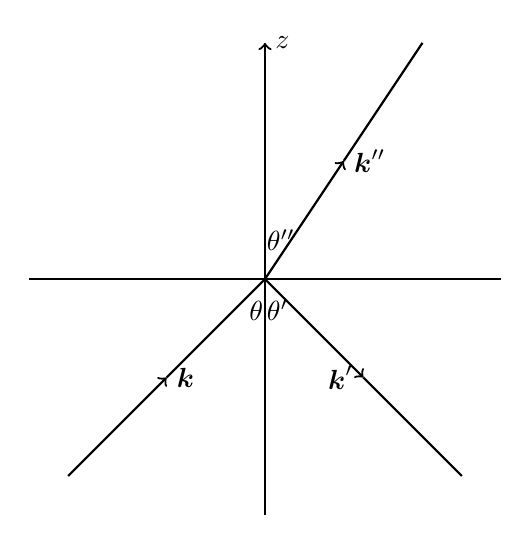
\begin{tikzpicture}
		\draw[thick] (-3,0)--(3,0);
		\draw[->,thick] (0,-3)--(0,3)node[anchor=west]{$z$};
		\draw[->,thick] (-2.5,-2.5)--(-1.25,-1.25)node[anchor=west]{$\b{k}$};
		\draw[thick] (-1.25,-1.25)--(0,0);
		\draw[->,thick] (0,0)--(1.25,-1.25)node[anchor=east]{$\b{k}'$};
		\draw[thick] (1.25,-1.25)--(2.5,-2.5);
		\draw[->,thick](0,0)--(1,1.5)node[anchor=west]{$\b{k}''$};
		\draw[thick](1,1.5)--(2,3);
		\draw (0.1,-0.4)node[anchor=east]{$\theta$};
		\draw (-0.1,-0.4)node[anchor=west]{$\theta'$};
		\draw (-0.1,0.5)node[anchor=west]{$\theta''$};
	\end{tikzpicture}
	\end{figure}
	考虑平面波解,
	\[\b{E}=\b{E}_0\e^{\i(\b{k}\cdot\b{r}-\omega t)},\]
	那么反射波和透射波可以分别表示为
	\[\b{E}'=\b{E}'_0\e^{\i(\b{k}'\cdot\b{r}-\omega' t)},\quad \b{E}''=\b{E}''_0\e^{\i(\b{k}''\cdot\b{r}-\omega'' t)},\]

	根据边值关系,可以得到以下方程
	\[\hat{\b{e}}_z\times\b{E}+\hat{\b{e}}_z\times\b{E}'=\hat{\b{e}}_z\times\b{E}'',\]
	我们在垂直于$\hat{\b{e}}_z$的平面上定义两个正交单位矢量,使得
	\[\hat{\b{e}}_t\times\hat{\b{e}}_b=\hat{\b{e}}_z,\quad \hat{\b{e}}_b\times\hat{\b{e}}_z=\hat{\b{e}}_t,\quad \hat{\b{e}}_z\times\hat{\b{e}}_t=\hat{\b{e}}_b.\]
	利用这个关系我们有
	\[\hat{\b{e}}_b\cdot(\hat{\b{e}}_z\times\b{E})=\b{E}\cdot(\hat{\b{e}}_b\times\hat{\b{e}}_z)=\b{E}\cdot\b{e}_t=\b{E}_t,\]
	因此上面的式子可以写为
	\[E_{0t}\e^{\i(\b{k}\cdot\b{r}-\omega t)}+E'_{0t}\e^{\i(\b{k}'\cdot\b{r}-\omega' t)}=E''_{0t}\e^{\i(\b{k}''\cdot\b{r}-\omega'' t)}.\]
	注意到,我们这里引入的这一组基矢量是可以任选的,因此上面这个式子对于电场垂直于$\hat{\b{e}}_z$的任何一个分量都成立。
	
	接下来进行一些操作。先考察各个波之间频率的关系,由于$\b{r}$可以取任意值,故令$\b{r}=0$,则
	\[E_{0t}\e^{-\i\omega t}+E'_{0t}\e^{-\i\omega' t}=E''_{0t}\e^{-\i\omega'' t}.\]
	对这个式子可以进一步进行两种处理,一种是直接令$t=0$,另一种是两边对$t$求导而后再令$t=0$,这样可以得到两个方程
	\[E_{0t}+E'_{0t}=E''_{0t},\]
	\[E_{0t}\omega+E'_{0t}\omega'=E''_{0t}\omega''.\]
	对比就可以得到频率之间的相互关系
	\[\omega=\omega'=\omega''.\]
	这一步其实是从一开始就可以从物理上分析出来的。
	
	再取$t=0$,$y=0$,则
	\[E_{0t}\e^{\i k_x x}+E'_{0t}\e^{\i k'_x x}=E''_{0t}\e^{\i k''_x x},\]
	同样的进行两种不同的操作,再联立所得的方程,就可以得到
	\[k_x=k_x'=k_x'',\quad \Rightarrow k_y=k_y'=k_y''.\]
	不妨假设$k_y=0$,此时通过几何关系就有
	\[k_x=k\sin\theta=\omega\sqrt{\mu_1\varepsilon_1}\sin\theta,\quad k_x'=k'\sin\theta=\omega\sqrt{\mu_1\varepsilon_1}\sin\theta',\quad k_x''=k''\sin\theta=\omega\sqrt{\mu_2\varepsilon_2}\sin\theta'',\]
	\[\sin\theta=\sin\theta',\qquad \frac{\sin\theta}{\sin\theta''}=\sqrt{\frac{\mu_2\varepsilon_2}{\mu_1\varepsilon_1}}=\frac{n_2}{n_1}=n_{21}.\]
	这就是我们所熟知的折射定律。
	
	\subsection{振幅关系}
	我们将电磁波分解为两个方向来研究各个波之间振幅的关系。
	\begin{figure}[H]
		\centering
		\subfigure[$\b{E}$垂直于入射面]{
			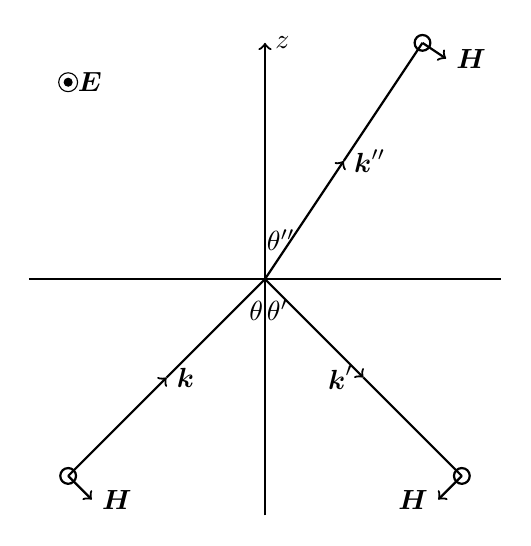
\begin{tikzpicture}
				\draw[thick] (-3,0)--(3,0);
				\draw[->,thick] (0,-3)--(0,3)node[anchor=west]{$z$};
				\draw[->,thick] (-2.5,-2.5)--(-1.25,-1.25)node[anchor=west]{$\b{k}$};
				\draw[thick] (-1.25,-1.25)--(0,0);
				\draw[->,thick] (0,0)--(1.25,-1.25)node[anchor=east]{$\b{k}'$};
				\draw[thick] (1.25,-1.25)--(2.5,-2.5);
				\draw[->,thick](0,0)--(1,1.5)node[anchor=west]{$\b{k}''$};
				\draw[thick](1,1.5)--(2,3);
				\draw[->,thick](-2.5,-2.5)--(-2.2,-2.8)node[anchor=west]{$\b{H}$};
				\draw[->,thick](2.5,-2.5)--(2.2,-2.8)node[anchor=east]{$\b{H}$};
				\draw[->,thick](2,3)--(2.3,2.8)node[anchor=west]{$\b{H}$};
				\draw[thick](-2.5,-2.5)ellipse(0.1 and 0.1);
				\draw[thick](2.5,-2.5)ellipse(0.1 and 0.1);
				\draw[thick](2,3)ellipse(0.1 and 0.1);
				\draw (0.1,-0.4)node[anchor=east]{$\theta$};
				\draw (-0.1,-0.4)node[anchor=west]{$\theta'$};
				\draw (-0.1,0.5)node[anchor=west]{$\theta''$};
				\filldraw (-2.5,2.5) ellipse(0.05 and 0.05);
				\draw (-2.5,2.5) ellipse(0.12 and 0.12);
				\draw (-2.5,2.5)node[anchor=west]{$\b{E}$};
				
			\end{tikzpicture}
		}
		\subfigure[$\b{E}$平行于入射面]{
			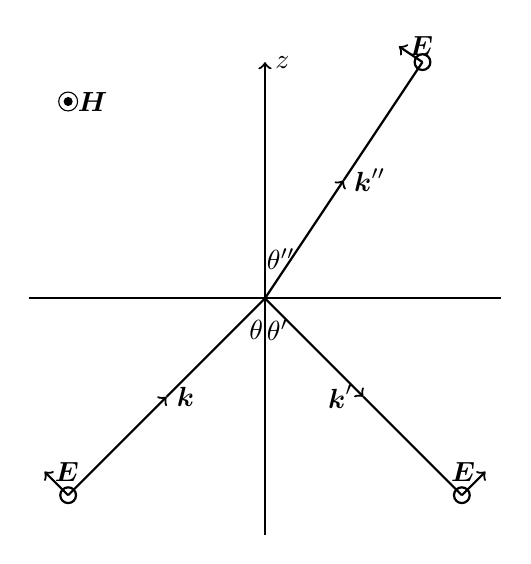
\begin{tikzpicture}
				\draw[thick] (-3,0)--(3,0);
				\draw[->,thick] (0,-3)--(0,3)node[anchor=west]{$z$};
				\draw[->,thick] (-2.5,-2.5)--(-1.25,-1.25)node[anchor=west]{$\b{k}$};
				\draw[thick] (-1.25,-1.25)--(0,0);
				\draw[->,thick] (0,0)--(1.25,-1.25)node[anchor=east]{$\b{k}'$};
				\draw[thick] (1.25,-1.25)--(2.5,-2.5);
				\draw[->,thick](0,0)--(1,1.5)node[anchor=west]{$\b{k}''$};
				\draw[thick](1,1.5)--(2,3);
				\draw[->,thick](-2.5,-2.5)--(-2.8,-2.2)node[anchor=west]{$\b{E}$};
				\draw[->,thick](2.5,-2.5)--(2.8,-2.2)node[anchor=east]{$\b{E}$};
				\draw[->,thick](2,3)--(1.7,3.2)node[anchor=west]{$\b{E}$};
				\draw[thick](-2.5,-2.5)ellipse(0.1 and 0.1);
				\draw[thick](2.5,-2.5)ellipse(0.1 and 0.1);
				\draw[thick](2,3)ellipse(0.1 and 0.1);
				\draw (0.1,-0.4)node[anchor=east]{$\theta$};
				\draw (-0.1,-0.4)node[anchor=west]{$\theta'$};
				\draw (-0.1,0.5)node[anchor=west]{$\theta''$};
				\filldraw (-2.5,2.5) ellipse(0.05 and 0.05);
				\draw (-2.5,2.5) ellipse(0.12 and 0.12);
				\draw (-2.5,2.5)node[anchor=west]{$\b{H}$};
			\end{tikzpicture}
		}
	\end{figure}
	我们用下标$\perp,||$分别表示垂直于和平行于入射面的分量。
	\subsubsection{$\b{E}$垂直于入射面}
	\[\hat{\b{e}}_z\times(\b{E}_2-\b{E}_1)=0\quad\Rightarrow \quad E_{\perp}+E_{\perp}'=E_{\perp}'',\]
	\[\hat{\b{e}}_z\times(\b{H}_2-\b{H}_1)=0\quad\Rightarrow \quad=H_{||}\cos\theta-H_{||}'\cos\theta'=H_{||}''\cos\theta''.\]
	利用关系
	\[H=\sqrt{\frac{\varepsilon}{\mu}}E,\quad \theta=\theta',\]
	并且假定
	\[\mu_1=\mu_2=\mu_0,\]
	这就有
	\[\frac{E_{\perp}'}{E_{\perp}}=-\frac{\sin(\theta-\theta'')}{\sin(\theta+\theta'')},\quad \frac{E_{\perp}''}{E_{\perp}}=\frac{2\cos\theta\sin\theta''}{\sin(\theta+\theta'')}.\]
	
	\subsubsection{$\b{E}$平行于入射面}
	进行类似的分析可以得到类似的公式
	\[\frac{E_{||}'}{E_{||}}=\frac{\tan(\theta-\theta'')}{\tan(\theta+\theta'')},\quad \frac{E_{||}''}{E_{||}}=\frac{2\cos\theta\sin\theta''}{\sin(\theta+\theta'')\cos(\theta-\theta'')}.\]
	这四个公式就是光学中的菲涅尔公式。
	
	\subsection{全反射}
	当电磁波从光密介质射向光疏介质时($\varepsilon_1>\varepsilon_2$),入射角将有一个最大值,超过这个角时,折射角没有实数解。我们来考虑发生这种现象时折射波的行为。
	\[k=\omega\sqrt{\mu_1\varepsilon_1},\quad k''=\omega\sqrt{\mu_2\varepsilon_2},\]
	设
	\[k_x=k_x''=k\sin\theta,\quad k_y=k_y''=0,\]
	可以解出
	\[k_z''=\sqrt{k''^2-k''^2_x}=\i k\sqrt{\sin^2\theta-n_{21}^2}=\i\lambda,\]
	于是折射波电场即表现为一个指数衰减的情形
	\[\b{E}''=\b{E}_0''\e^{-\lambda z}\e^{\i(k_x'' x-\omega t)}.\]
	考虑折射波的能流密度,为了简化,我们设$\b{E}''=E''_y\hat{\b{e}}_y$,则相应的磁场强度
	\[\b{H}''=\frac{\b{B}''}{\mu_2}=\sqrt{\frac{\varepsilon_2}{\mu_2}}\hat{\b{e}}_k''\times\b{E}''=\sqrt{\frac{\varepsilon_2}{\mu_2}}\frac{k''_x\hat{\b{e}}_y-\i\lambda\hat{\b{e}}_x}{k''}E''_y\e^{-\lambda z}\e^{\i(k''_x x-\omega t)},\]
	
	\section{导电介质的电磁波}
	\subsection{导体内自由电荷的分布}
	电荷守恒
	\[\nabla\cdot\b{j}+\frac{\partial \rho}{\partial t}=0,\]
	欧姆定理
	\[\b{j}=\sigma\b{E},\]
	电位移矢量满足的散度方程以及线性介质满足的关系
	\[\nabla\cdot\b{D}=\rho_f,\quad \b{D}=\varepsilon\b{E},\]
	于是有
	\[\frac{\partial \rho}{\partial t}=-\frac{\sigma}{\varepsilon}\rho\quad\Rightarrow \quad \rho(\b{r},t)=\rho(\b{r},t=0)\e^{-\frac{\sigma}{\varepsilon}t},\]
	对于良导体,$\sigma$非常大,因此可以认为导体内部$\rho=0$。
	
	\subsection{导体内Maxwell方程及单色电磁波}
	相比真空中的电磁波方程,导体中的电磁波方程表现为增加了电流密度项。从增加了传导电流密度项的真空中无源Maxwell方程出发
	\[\nabla\times\b{E}=-\frac{\partial \b{B}}{\partial t},\quad \nabla\times\b{H}=\b{j}+\frac{\partial \b{D}}{\partial t},\quad \nabla\cdot\b{D}=\nabla\cdot\b{B}=0.\]
	考虑单色波$\b{E}(\b{r},t)=\b{E}(\b{r})\e^{-\i\omega t},\b{B}(\b{r},t)=\b{B}(\b{r})\e^{-\i\omega t}$以及线性关系$\b{D}=\varepsilon\b{E},\b{B}=\mu\b{H}$,则代入上述导体中的电磁波方程后有
	\[\nabla\times\b{E}(\b{r})=\i\omega\mu\b{H}(\b{r}),\]
	\[\nabla\times\b{H}(\b{r})=-\i\omega\varepsilon\b{E}(\b{r})+\sigma\b{E}(\b{r})=-\i\omega\tilde{\varepsilon}\b{E}(\b{r}),\]
	这里定义了复的介电常数
	\[\tilde{\varepsilon}\triangleq\varepsilon+\i\frac{\sigma}{\omega}.\]
	类似于介质中电磁波的推导
	\[\nabla\times(\nabla\times\b{E})=\omega^2\mu\tilde{\varepsilon}\b{E},\]
	定义一个复的波矢,使得
	\[\tilde{k}\triangleq\omega\sqrt{\mu\tilde{\varepsilon}},\]
	这样就得到
	\[\left\{\begin{aligned}
		\nabla^2\b{E}+\tilde{k}^2\b{E}&=0,\\
		\nabla\cdot\b{E}&=0,\\
		\b{H}&=-\frac{\i}{\omega\mu}\nabla\times\b{E}.
	\end{aligned}\right.\]
	我们假设复波矢可以写成这样的形式
	\[\tilde{\b{k}}=\b{\beta}+\i\b{\alpha},\]
	那么
	\[\b{E}(\b{r},t)=\b{E}_{0k}\e^{-\b{\alpha}\cdot\b{r}}\e^{\i(\b{\beta}\cdot\b{r}-\omega t)},\]
	可以看到,复的波矢导致了一个衰减因子。对照复介电常数的定义我们可以得到复波矢实部和虚部满足的方程
	\[\beta^2-\alpha^2=\omega^2\mu\varepsilon,\quad \b{\alpha}\cdot\b{\beta}=\frac{1}{2}\omega\mu\sigma.\]
	
	\subsection{趋肤效应和穿透深度}
	简单起见,我们考虑$\b{\alpha}//\b{\beta}$,$z=0$为导体表面,$\b{\alpha},\b{\beta}$沿$z$方向,于是
	\[\b{E}=\b{E}_{0k}\e^{-\alpha z}\e^{-\i(\beta z - \omega t)},\]
	同时在这样给定了边值条件之后我们可以将$\alpha,\beta$具体地求出
	\[\alpha=\omega\sqrt{\frac{\mu\varepsilon}{2}}\left(\sqrt{1+\left(\frac{\sigma}{\varepsilon\omega}\right)^2}-1\right)^{\frac{1}{2}},\]
	\[\beta=\omega\sqrt{\frac{\mu\varepsilon}{2}}\left(\sqrt{1+\left(\frac{\sigma}{\varepsilon\omega}\right)^2}+1\right)^{\frac{1}{2}}.\]
	对于良导体,有$\sigma \gg \varepsilon \omega$,因此
	\[\alpha\approx\beta\approx \sqrt{\frac{\omega \mu\sigma}{2}}.\]
	穿透深度定义为
	\[\delta=\frac{1}{\alpha}=\sqrt{\frac{2}{\omega\mu\sigma}}.\]
	
	考察$\b{E}$与$\b{H}$之间的关系
	\[\b{H}=\frac{1}{\i\omega \mu}\nabla\times\b{E}=\frac{1}{\omega\mu}\tilde{\b{k}}\times\b{E}\approx\sqrt{\frac{\sigma}{\omega\mu}}\e^{\i\frac{\pi}{4}}\hat{\b{e}}_z\times\b{E}.\]
	这里使用了良导体中复波矢的条件。可以看到,电场与磁场相差$\pi/4$的相位。由此考察良导体中能量密度在电场和磁场之间的分配
	\[\frac{\mu H^2}{\varepsilon E^2}=\frac{\mu}{\varepsilon}\frac{\sigma}{\omega \mu}=\frac{\sigma}{\varepsilon\omega} \gg 1.\]
	可见,在良导体中,电磁波能量中磁场占主导地位。
	
	\section{谐振腔}
	
	\subsection{有限空间的电磁波}
	仍然考虑单频时谐电磁波$\b{E}(\b{r},t)=\b{E}(\b{r})\e^{-\i\omega t},\b{B}(\b{r},t)=\b{B}(\b{r})\e^{-\i\omega t}$,那么我们要解的方程就变成
	\[\left\{\begin{aligned}
		\nabla^2\b{E}+\mu\varepsilon\omega^2\b{E}&=0,\\
		\nabla^2\b{B}+\mu\varepsilon\omega^2\b{B}&=0,
	\end{aligned}\right.\quad + \quad \text{边界条件}\]
	边界条件由我们要求解的有限区域特征给出。
	
	\subsection{理想导体的边界条件}
	我们已经知道,麦克斯韦方程组给出四个边界条件方程
	\[\hat{\b{n}}\cdot(\b{D}_2-\b{D}_1)=\sigma,\qquad \hat{\b{n}}\cdot(\b{B}_2-\b{B}_1)=0,\]
	\[\hat{\b{n}}\times(\b{E}_2-\b{E}_1)=0,\qquad \hat{\b{n}}\times(\b{H}_2-\b{H}_1)=\b{\alpha}.\]
	对于理想导体,我们可以认为$\b{E}_1=\b{H}_1=0$,因此电磁波边界条件化为
	\[\hat{\b{e}}_n\times\b{E}=0,\quad \hat{\b{e}}_n\times\b{H}=\b{\alpha},\quad \hat{\b{e}}_n\cdot\b{D}=\sigma,\quad \hat{\b{e}}_n\cdot\b{B}=0.\]
	
	\subsection{矩形谐振腔}
	\begin{figure}[H]
		\centering
		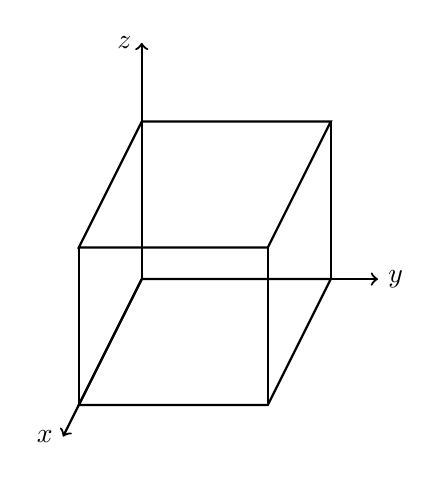
\begin{tikzpicture}
			\draw[->,thick](0,0)--(-1,-2)node[anchor=east]{$x$};
			\draw[->,thick](0,0)--(3,0)node[anchor=west]{$y$};
			\draw[->,thick](0,0)--(0,3)node[anchor=east]{$z$};
			\draw[thick](0,0)--(-0.8,-1.6)--(1.6,-1.6)--(2.4,0)--(0,0);
			\draw[thick](0,2)--(-0.8,0.4)--(1.6,0.4)--(2.4,2)--(0,2);
			\draw[thick](0,0)--(0,2);
			\draw[thick](-0.8,-1.6)--(-0.8,0.4);
			\draw[thick](1.6,-1.6)--(1.6,0.4);
			\draw[thick](2.4,0)--(2.4,2);
		\end{tikzpicture}
		\caption{谐振腔示意图}
	\end{figure}
	在矩形谐振腔下,我们自然地选取直角坐标系并进行分离变量。要求解的方程可以写为
	\[\nabla^2 u+k^2u=0,\]
	其中$u$代表$E_x,E_y,E_z$中的任何一个分量。分离变量
	\[u(x,y,z)=X(x)Y(y)Z(z),\]
	就得到
	\[\frac{\d^2 X}{\d x^2}+k_x^2X^2=0,\quad \quad \frac{\d^2 Y}{\d y^2}+k_y^2Y^2=0,\frac{\d^2 Z}{\d z^2}+k_z^2Z^2=0,\]
	其中参数满足关系
	\[k_x^2+k_y^2+k_z^2=k^2=\omega^2\mu\varepsilon.\]
	考虑边界条件,先考察与$z$轴垂直的切面,则应该有
	\[E_x|_{z=0}=E_x|_{z=l_3}=E_y|_{z=0}=E_y|_{z=l_3}=0,\]
	由横波条件(即散度方程),我们应该有
	\[\nabla\cdot\b{E}|_{z=0}=\nabla\cdot\b{E}|_{z=l_3}=0,\]
	而同时我们由我们先前得到的在$z$方向边界上的恒等条件,我们有
	\[\left.\frac{\partial E_x}{\partial x}\right|_{z=0}=\left.\frac{\partial E_y}{\partial y}\right|_{z=0}=\left.\frac{\partial E_x}{\partial x}\right|_{z=l_3}=\left.\frac{\partial E_y}{\partial y}\right|_{z=l_3}=0,\]
	从而将这两项从散度方程中删去,横波条件给出的边界条件就可以写成
	\[\left.\frac{\partial E_z}{\partial z}\right|_{z=0}=\left.\frac{\partial E_z}{\partial z}\right|_{z=l_3}=0.\]
	类似地,可以得到与$y$轴、$x$轴垂直的切面上需满足的边界条件。
	\[E_x|_{y=0}=E_x|_{y=l_2}=E_z|_{y=0}=E_z|_{y=l_2}=0,\]
	\[\left.\frac{\partial E_y}{\partial y}\right|_{z=0}=\left.\frac{\partial E_y}{\partial y}\right|_{z=l_2}=0,\]
	\[E_y|_{x=0}=E_y|_{x=l_1}=E_z|_{x=0}=E_z|_{x=l_1}=0,\]
	\[\left.\frac{\partial E_x}{\partial x}\right|_{x=0}=\left.\frac{\partial E_x}{\partial x}\right|_{x=l_1}=0.\]
	将这些边界条件带入到分离变量的本征值问题中,不难得到一般解
	\[E_x(x,y,z)=A_1\cos k_xx\sin k_yy\sin k_zz,\]
	\[E_y(x,y,z)=A_2\sin k_xx\cos k_yy\sin k_zz,\]
	\[E_z(x,y,z)=A_3\sin k_xx\sin k_yy\cos k_zz,\]
	其中
	\[k_x=\frac{\pi m}{l_1},\quad k_y=\frac{\pi n}{l_2},\quad k_z=\frac{\pi p}{l_3},\quad m,n,p = 0,1,2,\dots\]
	应当注意这里的$A_1,A_2,A_3$不是完全独立的,这可以由横波条件给出
	\[\nabla\cdot\b{E}=A_1k_x+A_2k_y+A_3k_z,\]
	可以看到只有两个是相互独立的,这也可以从偏振自由度中看出。
	
	谐振腔的本征频率满足
	\[\omega_{mnp}=\frac{\pi}{\sqrt{\mu\varepsilon}}\sqrt{\left(\frac{m}{l_1}\right)^2+\left(\frac{n}{l_2}\right)^2+\left(\frac{p}{l_3}\right)^2}.\]
	
	\section{波导}
	\begin{figure}[H]
	\centering
	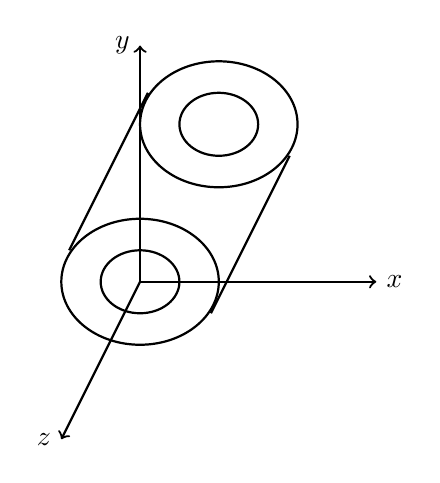
\begin{tikzpicture}
		\draw[->,thick](0,0)--(-1,-2)node[anchor=east]{$z$};
		\draw[->,thick](0,0)--(3,0)node[anchor=west]{$x$};
		\draw[->,thick](0,0)--(0,3)node[anchor=east]{$y$};
		\draw [thick](0,0)ellipse(0.5 and 0.4);
		\draw [thick](0,0)ellipse(1 and 0.8);
		\draw [thick](-0.9,0.4)--(-0.9+1,0.4+2);
		\draw [thick](0.9,-0.4)--(0.9+1,-0.4+2);
		\draw [thick](1,2)ellipse(0.5 and 0.4);
		\draw [thick](1,2)ellipse(1 and 0.8);
	\end{tikzpicture}
	\caption{波导示意图}
	\end{figure}
	波导可以看成是给波动方程的定解问题构成在一个方向上无限且具有平移不变的边界条件。
	
	\subsection{场量按平行和垂直传播方向分解}
	由于柱型波导在$z$方向具有平移不变性,因此可以设$z$方向为平面波形式
	\[\b{E}(\b{r},t)=\b{E}_0(x,y)\e^{\pm\i k_zz-\i\omega t},\quad \b{B}(\b{r},t)=\b{B}_0(x,y)\e^{\pm\i k_zz-\i\omega t},\]
	在直角坐标系下,拉普拉斯算符写为$z$方向与切向($t$)两部分
	\[\nabla^2=\frac{\partial^2}{\partial x^2}+\frac{\partial^2}{\partial y^2}+\frac{\partial^2}{\partial z^2}=\nabla_t^2+\nabla_z^2.\]
	代入到我们设的解中,由波动方程有
	\[(\nabla_t^2+\mu\varepsilon\omega^2-k_z^2)\b{E}_0(x,y)\e^{\pm\i k_zz-\i\omega t}=0.\]
	将电磁场也分解为两部分
	\[\b{E}=E_z\hat{\b{e}}_z+\b{E}_t,\quad \b{B}=B_z\hat{\b{e}}_z+\b{B}_t\]
	由我们已经多次用过的时谐电磁波满足的方程
	\[\nabla\times\b{E}=\i\omega\b{B},\quad \nabla\times\b{B}=-\i\omega\varepsilon\mu\b{E},\]
	我们可以说明,切向的电场分量可以由$z$方向的电场求解出来
	\[\b{E}_t=\frac{\pm\i}{\omega^2\mu\varepsilon-k_z^2}\left[k_z\nabla_tE_z\mp\omega(\hat{\b{e}}_z\times\nabla_t)B_z\right],\]\label{*1}
	\[\b{B}_t=\frac{\pm\i}{\omega^2\mu\varepsilon-k_z^2}\left[k_z\nabla_tB_z\pm\omega(\hat{\b{e}}_z\times\nabla_t)E_z\right],\]\label{*2}
	\begin{proof}
		首先将时谐电磁波的两个方程按照切向和$z$方向分开写出来
		\[(\nabla_t+\nabla_z)\times(\b{E}_t+\b{E}_z)=\i\omega(\b{B}_t+\b{B}_z),\]
		\[(\nabla_t+\nabla_z)\times(\b{B}_t+\b{B}_z)=-\i\omega\varepsilon\mu(\b{E}_t+\b{E}_z),\]
		其中注意到,
		\[\nabla_z\times\b{E}_z=\begin{vmatrix} \hat{\b{e}}_x & \hat{\b{e}}_y & \hat{\b{e}}_z \\ 0 & 0 & \partial_z \\ 0 & 0 & E_z \end{vmatrix}=0,\]
		
		根据分量之间的对应关系可以整理出四个方程
		\[\nabla_t\times\b{E}_z=\i\omega\b{B}_z,\quad \nabla_t\times\b{E}_z+\nabla_z\times\b{E}_t=\i\omega\b{B}_t,\]
		\[\nabla_t\times\b{B}_t=-\i\omega\varepsilon\mu\b{E}_z,\quad \nabla_t\times\b{B}_z+\nabla_z\times\b{B}_t=-\i\omega\varepsilon\mu\b{E}_t.\]
		
		将右上角的式子左右两边取$\nabla_z$的旋度,先计算左边
		\[\nabla_z\times(\nabla_t\times\b{E}_z)=\nabla_t(\nabla\cdot\b{E}_z)-(\nabla_z\cdot\nabla_t)\b{E}_z = \nabla_t\left(\frac{\partial E_z}{\partial z}\right),\]
		\[\nabla_z\times(\nabla_z\times\b{E}_t)=\nabla_z(\nabla_z\cdot\b{E}_t)-\nabla_z^2\b{E}_t=-\nabla_z^2\b{E}_t,\]
		因此
		\[\nabla_t\left(\frac{\partial E_z}{\partial z}\right) -\nabla_z^2\b{E}_t=\i\omega\nabla_z\times\b{B}_t. \]
		
		同理,处理右下角的式子可以得到
		\[\nabla_t\left(\frac{\partial B_z}{\partial z}\right)-\nabla_z^2\b{B}_t=-\i\omega\varepsilon\mu\nabla_z\times\b{E}_t.\]
		
		同时,在时谐情况下,我们有
		\[\nabla_z^2\b{E}_t=\frac{\partial^2}{\partial z^2}\b{E}_{0t}(x,y)\e^{\pm\i k_z z - \i\omega t}=-k_z^2\b{E}_t,\]
		因此上面两个方程可以改写成
		\[\nabla_t\left(\frac{\partial E_z}{\partial z}\right) +k_z^2\b{E}_t=\i\omega\nabla_z\times\b{B}_t,\]
		\[\nabla_t\left(\frac{\partial B_z}{\partial z}\right)+k_z^2\b{B}_t=-\i\omega\varepsilon\mu\nabla_z\times\b{E}_t.\]
		将右下角的式子代入到上面第一个式子中,右上角的式子代入到上面第二个式子中,我们就得到
		\[\nabla_t\left(\frac{\partial E_z}{\partial z}\right)+\i\omega\nabla_t\times\b{B}_z=(\omega^2\mu\varepsilon-k_z^2)\b{E}_t,\]
		\[\nabla_t\left(\frac{\partial B_z}{\partial z}\right)-\i\omega\varepsilon\mu\nabla_t\times\b{E}_z=(\omega^2\mu\varepsilon-k_z^2)\b{B}_t,\]
		时谐情形下我们有关系
		\[\frac{\partial E_z}{\partial z}=\pm\i k_z E_z,\]
		并且
		\[\nabla_t\times\b{E}_z=(\hat{\b{e}}_z\times\nabla_t)E_z,\]
		因此就可以整理得到
		\[\b{E}_t=\frac{\pm\i}{\omega^2\mu\varepsilon-k_z^2}\left[k_z\nabla_tE_z\mp\omega(\hat{\b{e}}_z\times\nabla_t)B_z\right],\]
		\[\b{B}_t=\frac{\pm\i}{\omega^2\mu\varepsilon-k_z^2}\left[k_z\nabla_tB_z\pm\omega(\hat{\b{e}}_z\times\nabla_t)E_z\right].\]
		证毕。
	\end{proof}
	
	在实用中,我们常常考虑两种情况
	\begin{itemize}
		\item $E_z=0$,横电波(TE模式);
		\item $B_z=0$,横磁波(TM模式)。
	\end{itemize}
	横电磁波(即$E_z,B_z$同时为零)可以被证明是不可能的。
	
	\subsection{纵向分量$E_z,B_z$的边界条件}
	从电磁场最一般的边界条件出发,考虑波导的情况。波导内部(记为介质2)可以是真空,也可以是介质,外部(记为介质1)可以认为是导体。于是有
	\[\b{E}_1=0,\quad \b{H}_1=0.\]
	这样就有
	\[\hat{\b{e}}_n\times\b{E}=0\quad \Rightarrow E_z|_s=0,\]
	
	\[\hat{\b{e}}_n\cdot\b{B}=0\quad \Rightarrow \hat{\b{e}}_n\cdot\b{B}_t|s=0,\]
	而由上一节中推出的公式,
	\[\hat{\b{e}}_n\cdot\b{B}_t\sim k_z\hat{\b{e}}_n\cdot\nabla_t B_z\pm\omega\hat{\b{e}}_n\cdot(\hat{\b{e}}_n\times\nabla_t)E_z \sim \frac{\partial B_z}{\partial n},\]
	所以
	\[\left.\frac{\partial B_z}{\partial n}\right|_s=0,\]
	
	接下来就要求解在上述边界条件下的二维空间中的亥姆霍兹方程
	\[\left\{\begin{aligned}
		(\nabla^2_t+\mu\varepsilon\omega^2-k_z^2)E_{0z}(x,y)&=0 \\
		(\nabla^2_t+\mu\varepsilon\omega^2-k_z^2)B_{0z}(x,y)&=0 \\
	\end{aligned}\right.\]
	若已求得$E_{0z},B_{0z}$,那么就可以利用\ref{*1}\ref{*2}来求得切向的分量
	\[E_x=\frac{\i}{k_t^2}\left[k_z\frac{\partial E_z}{\partial x}+\omega\frac{\partial B_z}{\partial y}\right],\]
	\[E_y=\frac{\i}{k_t^2}\left[k_z\frac{\partial E_z}{\partial y}-\omega\frac{\partial B_z}{\partial x}\right],\]
	\[B_x=\frac{\i}{k_t^2}\left[k_z\frac{\partial B_z}{\partial x}-\omega\mu\varepsilon\frac{\partial E_z}{\partial y}\right],\]
	\[B_y=\frac{\i}{k_t^2}\left[k_z\frac{\partial B_z}{\partial y}+\omega\mu\varepsilon\frac{\partial E_z}{\partial x}\right].\]
	如果在柱坐标下求解,则有
	\[E_\rho=\frac{\i}{k_t^2}\left[k_z\frac{\partial E_z}{\partial \rho}+\frac{\omega}{\rho}\frac{\partial B_z}{\partial \phi}\right],\]
	\[E_\phi=\frac{\i}{k_t^2}\left[\frac{k_z}{\rho}\frac{\partial E_z}{\partial \phi}-\omega\frac{\partial B_z}{\partial \rho}\right],\]
	\[B_\rho=\frac{\i}{k_t^2}\left[k_z\frac{\partial B_z}{\partial \rho}-\frac{\omega\varepsilon\mu}{\rho}\frac{\partial E_z}{\partial \phi}\right],\]
	\[B_\phi=\frac{\i}{k_t^2}\left[\frac{k_z}{\rho}\frac{\partial B_z}{\partial \phi}+\omega\mu\varepsilon\frac{\partial E_z}{\partial \rho}\right].\]
	
	\subsection{矩形波导的求解}
	
	我们分成两种模式来讨论。
	\subsubsection{TE模}
	分离变量
	\[B_{0z}(x,y)=X(x)Y(y),\]
	则
	\[\frac{\d^2X}{\d x^2}+k_x^2X=0,\quad \frac{\d^2y}{\d y^2}+k_y^2Y=0,\quad k_x^2+k_y^2+k_z^2=\omega^2\mu\varepsilon.\]
	通解
	\[\left\{\begin{aligned}
		X(x)&=C_1\sin(k_x x)+D_1\cos(k_x x), \\
		Y(y)&=C_2\sin(k_y y)+D_2\cos(k_y y),		
	\end{aligned}\right.\]
	由边界条件,应该有
	\[C_1=0,\quad k_x=\frac{m\pi}{a},\quad m=0,1,2,\dots\]
	\[C_2=0,\quad k_y=\frac{n\pi}{b},\quad n=0,1,2,\dots\]
	于是就有
	\[\left\{\begin{aligned}
		B_{0z}(x,y)&=B_0\cos\frac{m\pi}{a}x\cos\frac{n\pi}{b}y \\
		E_{0z}(x,y)&=0.
	\end{aligned}
	\right.\]
	利用\ref{*1}\ref{*2}就有
	\[\left\{\begin{aligned}
	E_{0x}&\sim \omega\frac{\partial B_z}{\partial y}\sim\cos \frac{m\pi}{a}x\sin\frac{n\pi}{b}y, \\
	E_{0y}&\sim \omega\frac{\partial B_z}{\partial x}\sim\sin \frac{m\pi}{a}x\cos\frac{n\pi}{b}y,	
	\end{aligned}
	\right.\]
	\[\left\{\begin{aligned}
		B_{0x}&\sim\sin\frac{m\pi}{a} x\cos\frac{n\pi}{b}y,\\
		B_{0y}&\sim\cos\frac{m\pi}{a} x\sin\frac{n\pi}{b}y,
	\end{aligned}\right.\]
	相应的$k_z$
	\[k_z=\sqrt{\omega^2\mu\varepsilon-\frac{m^2\pi^2}{a^2}-\frac{n^2\pi^2}{b^2}},\]
	为了使得电磁波能在波导中长距离传播,这要求它没有衰减,即$k_z$为实数,因此可以定义截止频率
	\[\omega_{mn}=\frac{\pi}{\mu\varepsilon}\sqrt{\frac{m^2}{a^2}+\frac{n^2}{b^2}},\]
	我们传播的波必须满足
	\[\omega>\omega_{mn}.\]
	
	\subsubsection{TM模}
	使用对称的解法可以得到
	
	
	
	
	波导中真实传播的电磁波可以表示为两种模式的叠加。
	
	
	\section{等离子体}
	\subsection{基本概念}
	我们知道当温度由低到高变化时,物体将经历固态-液态-气态的物相变化,而当温度继续升高时,物体就会发生电离,形成第四种物态——等离子体态,内部电子和离子都不再是束缚的。它在宇宙中是常见的。我们既要处理它的电磁性质,又有处理它具有流体性质的运动。
	
	\subsection{等离子体的库仑屏蔽}
	我们考虑热平衡下的等离子体。正离子密度分布$n_{ion}(\b{r})$,带点$Ze$,电子密度分布$n_e(\b{r})$。
	
	设原点处放置$+q$的静止电荷,$\rho(\b{r})=q\delta(\b{r})$,我们来求等离子体中电势$\varphi(\b{r})$。我们有静电场的泊松方程
	\[\nabla^2\varphi=\frac{1}{\varepsilon_0}[-Zen_{ion}(\b{r})+en_e(\b{r})-q\delta(\b{r})],\]
	忽略正离子的运动,热平衡下, 电子在$\varphi(\b{r})$下服从玻尔兹曼分布(高温下玻尔兹曼分布是费米分布的一个好的近似)
	\[n_e(\b{r})=n_{e0}\exp\left[\frac{e\varphi(\b{r})}{k_BT}\right].\]
	我们采用高温近似,应该有$k_BT\gg e\varphi$,因此我们可以使用泰勒展开
	\[n_e(\b{r})=n_{e0}\left[1+\frac{e\varphi(\b{r})}{k_BT}\right],\]
	整体电中性要求应该有
	\[-Zen_{ion}+en_{e0}=0,\]
	于是泊松方程可以重新写为
	\[\left[\nabla^2-\frac{1}{\lambda^2}\right]\varphi(\b{r})=-\frac{q}{\varepsilon_0}\delta(\b{r}),\qquad \lambda^2=\frac{k_BT\varepsilon_0}{n_{e0}e^2},\]
	可以验证解为
	\[\varphi(\b{r})=\k\frac{q}{r}\e^{-\frac{r}{\lambda}}.\]
	称为德拜势。库仑屏蔽是等离子体最重要的性质。
	
	\subsection{等离子体振荡}
	电子的流体运动方程
	\[\frac{\partial n}{\partial t}+\nabla\cdot(n\b{v})=0.\]
	由牛顿运动定律
	\[mn\frac{\partial \b{v}}{\partial t}=-en\b{E},\]
	内电场
	\[\nabla\cdot\b{E}=-\frac{[n(\b{r})-n_0]e}{\varepsilon_0},\]
	考虑一个微振荡,即$n'=n-n_0$是一个小量,$\b{v}$也是一级小量。对运动方程两边去三度,并且将连续性方程代入就得到
	\[\frac{\partial^2 n'}{\partial t^2}+\frac{e^2n_0}{m\varepsilon}n'=0,\]
	可以解出
	\[n'(t)=n'(0)\e^{\i\omega_p t},\qquad \omega_p=\sqrt{\frac{e^2 n_0}{m\varepsilon_0}}.\]
	
	\subsection{电磁波在等离子体内的传播}
	仍然考虑微小振荡,忽略$\b{v}$在$\b{B}_e$下产生的效应。
	
	\chapter{电磁波的激发}
	本章中主要考虑宏观电磁波辐射的问题。
	
	\section{电磁势及方程}
	首先考虑电磁辐射的一般特征
	\[P=\oint \b{S}\cdot\d\b{a}=\frac{1}{\mu_0}\oint(\b{E}\times\b{B})\cdot\d\b{a},\]
	其中
	\[\d\b{a}\propto r^2,\quad \b{E},\b{B}\propto\frac{1}{r},\]
	由此可见电磁场的能量可以传播到无穷远处。下面进行具体的推导。
	
	\subsection{电磁场的矢势和标势}
	我们已经给出过电磁场矢势和标势的定义
	\[\b{B}=\nabla\times\b{A},\quad \nabla\varphi=-\b{E}-\frac{\partial \b{A}}{\partial t},\]
	这二者具有规范不变性
	\[\b{A}'=\b{A}+\nabla\Lambda,\quad \varphi'=\varphi-\frac{\partial \Lambda}{\partial t}.\]
	我们常常选择规范条件来处理具体问题。最常用的规范有库仑规范和洛伦兹规范,在讨论电磁波时,我们选用洛伦兹规范
	\[\nabla\cdot\b{A}+\mu_0\varepsilon_0\frac{\partial \varphi}{\partial t}=0.\]
	
	\subsection{电磁势方程}
	由上面给出的规范条件,我们可以推导出矢势和标势的波动方程
	\[\nabla^2\varphi-\mu_0\varepsilon_0\frac{\partial^2\varphi}{\partial t^2}=-\frac{\rho}{\varepsilon_0},\]
	\[\nabla^2\b{A}-\mu_0\varepsilon_0\frac{\partial^2 \b{A}}{\partial t^2}=-\mu_0\b{j}.\]
	这两个方程被称为\emph{达朗贝尔方程}。
	
	倘若选取库仑规范,则得到的方程为
	\[\nabla^2\varphi=-\frac{\rho}{\varepsilon_0},\]
	\[\nabla^2\b{A}-\frac{1}{c^2}\frac{\partial^2\b{A}}{\partial t^2}-\frac{1}{c^2}\frac{\partial \nabla\varphi}{\partial t}=-\mu\b{j}.\]
	
	\subsection{真空中的平面电磁波}
	\[\rho(\b{r})=0,\quad \b{j}(\b{r})=0,\]
	选取洛伦兹规范,我们可以写出平面波解
	\[\b{A}(\b{r},t)=\b{A}_{0k}\e^{\i(\b{k}\cdot\b{r}-\omega t)},\]
	\[\varphi(\b{r},t)=\varphi_{0k}\e^{\i(\b{k}\cdot\b{r}-\omega t)},\]
	洛伦兹规范给出二者之间的联系
	\[\varphi_{0k}=\frac{c^2}{\omega}\b{k}\cdot\b{A}_{ok},\]
	因此,在这种情况下只要给定矢量$\b{A}_0$就可以确定整个平面电磁波解。磁场
	\[\b{B}=\nabla\times\b{A}=\i\b{k}\times\b{A},\]
	电场
	\begin{align*}
		\b{E}&=-\nabla\varphi-\frac{\partial \b{A}}{\partial t} = -\i\b{k}\varphi+\i\omega\b{A} \\
		&=-\frac{\i c^2}{\omega}\left[\b{k}(\b{k}\cdot\b{A})-k^2\b{A}\right] \\
		&=-\frac{\i c^2}{\omega}\b{k}\times(\b{k}\times\b{A}) \\
		&=-c\hat{\b{e}}_k\times\b{B}.
	\end{align*}
	
	 从上面的讨论可以看出,整个解只依赖于矢势的垂直分量,这说明洛伦兹规范具有一定的剩余自由度,即沿平行方向。因此我们进一步假设,$\b{A}$只有横向部分,即$\b{k}\cdot\b{A}=0$,因此
	 \[\b{B}=\i\b{k}\times\b{A},\quad \b{E}=\i\omega\b{A}.\]
	 可以看到上面这个条件如果用库仑规范来做的话是可以自然得到的,但是这样的方便仅限于平面波解,在之后更复杂的问题中,我们还是选取更方便的洛伦兹规范,因为它使矢势和标势的方程具有对称性,在相对论中显示出协变性,因而对于理论探讨和实际计算都提供很大的方便。
	 
	 \section{电磁势的推迟解}
	 选取洛伦兹规范,获得先前推导出的达朗贝尔方程。由于标势和矢势分量的方程具有对称性,因此我们可以先求解标势的方程,而后自然地推出矢势分量地解。我们先从最简单的情况来表示
	 
	 \subsection{时变点电荷激发的标势}
	 假设
	 \[\rho(\b{r},t)=Q(t)\delta(\b{r}),\]
	 在$\b{r}\neq 0$处,标势满足拉普拉斯方程,写到球坐标系下,由于问题与$\theta,\phi$无关,因此
	 \[\frac{1}{r^2}\frac{\partial }{\partial r}\left(r^2\frac{\partial \varphi}{\partial t}\right)-\frac{1}{c^2}\frac{\partial^2\varphi}{\partial t^2}=0,\]
	 做替换
	 \[\varphi(\b{r},t)=\frac{U(\b{r},t)}{r},\]
	 于是
	 \[\frac{\partial^2U}{\partial r^2}-\frac{1}{c^2}\frac{\partial^2 U}{\partial t^2}=0.\]
	 由行波法,这个方程的通解可以写成
	 \[U(\b{r},t)=f(t-\frac{r}{c})+g(t+\frac{r}{c}),\]
	 第一项代表向外发射,第二项代代表向内收敛。在电磁辐射问题中,我们只考虑第一项,因此
	 \[\varphi(\b{r},t)=\frac{f(t-\frac{r}{c})}{r}.\]
	 构造一个尝试解
	 \[\varphi(\b{r},t)=\frac{Q\left(t-\frac{r}{c}\right)}{4\pi\varepsilon_0r},\]
	 可以验证,这个解可以回到静电势的情况。
	 
	 下面我们来说明这个解是满足非齐次的达朗贝尔方程的。以原点为中心取$\eta$为半径的球形区域,对达朗贝尔方程两边做体积分,则左边可以写为
	 \begin{align*}
	 	\int_0^\eta 4\pi r^2\d r \left(\nabla^2-\frac{1}{c^2}\frac{\partial^2}{\partial t^2}\right)\frac{Q\left(t-\frac{r}{c}\right)}{4\pi\varepsilon_0r}&=\frac{1}{\varepsilon_0}\int_0^\eta \d r\left[r\nabla^2 Q+r^2Q\nabla^2\frac{1}{r}+2r^2\nabla Q\cdot\nabla \frac{1}{r}-\frac{r}{c^2}\frac{\partial^2}{\partial t^2}Q\right] \\
	 	\text{取$\eta$趋于0的极限} &= \lim_{\eta\rightarrow 0}\frac{1}{\varepsilon_0}\int_0^\eta\d r r^2Q\nabla^2\frac{1}{r} \\
	 	&=\frac{Q}{4\pi\varepsilon_0}\lim_{\eta\rightarrow 0}\int\d V(-4\pi)\delta(\b{r}) \\
	 	&=-\frac{Q}{\varepsilon_0}.
	 \end{align*}
	因此,我们构造的尝试解是满足达朗贝尔方程的。
	
	倘若电荷不在原点上,而是位于$\b{r}'$处,那么相应的标势则为
	\[\varphi(\b{r},t)=\frac{1}{4\pi\varepsilon_0|\b{r}-\b{r}'|}Q\left(\b{r}',t-\frac{|\b{r}-\b{r}'|}{c}\right).\]
	
	\subsection{时变电荷电流分布的矢势与标势}
	由上一节中的结论,我们可以通过叠加原理得到一般的电荷分布$\rho(\b{r},t)$下的标势表达式
	\[\varphi(\b{r},t)=\k\int \d V' \frac{1}{|\b{r}-\b{r}'|}\rho\left(\b{r}',t-\frac{|\b{r}-\b{r}'|}{c}\right),\]
	由此可以对称地写出在一般电流密度分布$\b{j}(\b{r},t)$情况下的矢势表达式
	\[\b{A}(\b{r},t)=\frac{\mu_0}{4\pi}\int\d V'\frac{1}{|\b{r}-\b{r}'|}\b{j}\left(\b{r}',t-\frac{|\b{r}-\b{r}'|}{c}\right).\]
	
	从上面的表达式可以看出,电磁相互作用并不是瞬时和超距的,而是有一个推迟的作用,以光速传播,这也是我们将此解称为推迟势的原因。
	
	\subsection{洛伦兹规范的验证}
	这一节中我们来证明上面的两个推迟势解满足洛伦兹规范。首先复习复合函数的微分
	\[\nabla\cdot\b{f}(\b{r},a(\b{r}))=\nabla_r\cdot \b{f}+\nabla a\cdot\frac{\partial \b{f}}{\partial a}.\]
	这里第一个梯度算子的下标$r$不能略去,因为它代表对于$\b{r}$求偏导(而视$a$为常量),后边那个不带下标的梯度算子则是一般的对$\b{r}$求梯度。
	
	利用这个式子来计算矢势的散度。首先定义
	\[t'=t-\frac{|\b{r}-\b{r}'|}{c},\]
	于是
	\begin{align*}
		\nabla\cdot\b{A}(\b{r},t)&=\frac{\mu_0}{4\pi}\int\d V'\nabla\cdot\frac{\b{j}(\b{r'},t')}{|\b{r}-\b{r}'|} \\
		&=\frac{\mu_0}{4\pi}\int\d V'\left[\nabla_r\cdot\frac{\b{j}(\b{r}',t')}{|\b{r}-\b{r}'|}+\nabla t'\cdot\frac{\partial }{\partial t'}\frac{\b{j}(\b{r}',t')}{|\b{r}-\b{r}'|}\right]\\
		&=\frac{\mu_0}{4\pi}\int \d V'\left[\b{j}(\b{r}',t')\cdot\nabla\frac{1}{|\b{r}-\b{r}'|}+\nabla t'\cdot\frac{\partial }{\partial t'}\frac{\b{j}(\b{r}',t')}{|\b{r}-\b{r}'|}\right]\\
		&=\frac{\mu_0}{4\pi}\int \d V'\left[\frac{1}{|\b{r}-\b{r}'|}\nabla_r'\cdot\b{j}(\b{r}',t')-\nabla_r'\cdot\left(\frac{\b{j}(\b{r}',t')}{|\b{r}-\b{r}'|}\right)-\nabla' t'\cdot\frac{\partial }{\partial t'}\frac{\b{j}(\b{r}',t')}{|\b{r}-\b{r}'|}\right]\\
		&=\frac{\mu_0}{4\pi}\int\d V'\frac{1}{|\b{r}-\b{r}'|}\nabla_r'\cdot\b{j}-\frac{\mu_0}{4\pi}\oint\frac{\b{j}(\b{r}',t')}{|\b{r}-\b{r}'|}\cdot\d \b{S}' \\
		&=\frac{\mu_0}{4\pi}\int\d V'\frac{1}{|\b{r}-\b{r}'|}\nabla_r'\cdot\b{j}.
	\end{align*}
	这其中利用到了$\nabla_r'$的含义是对$\b{r}'$求偏导。对标势求偏导
	\[\frac{\partial }{\partial t}\varphi(\b{r},t)=\k\int\d V'\frac{\partial}{\partial t'}\rho(\b{r}',t'),\]
	于是
	\[\nabla\cdot\b{A}+\frac{1}{c^2}\frac{\partial }{\partial t}\varphi=\frac{\mu_0}{4\pi}\int\d V'\frac{1}{|\b{r}-\b{r}'|}\left[\nabla_r'\cdot\b{j}(\b{r}',t')+\frac{\partial}{\partial t'}\rho(\b{r}',t')\right]=0.\]
	最后一步使用了电荷守恒。由此我们就证明了推迟势解满足洛伦兹规范。(这部分的记号有点问题,回头再来纠正。)
	
	\subsection{另一种推导方法——含时格林函数法}
	这一部分主要是按照刘川的书和jackson的书来讲的。
	
	仍然从达朗贝尔方程出发,将两个方程简记为
	\[\nabla^2 \psi -\frac{1}{c^2}\frac{\partial^2 \psi}{\partial t^2}=-4\pi f(\b{r},t),\]
	做傅里叶变换
	\[\psi(\b{r},t)=\frac{1}{2\pi}\int_{-\infty}^\infty \tilde{\psi}(\b{r},\omega)\e^{-\i\omega t}\d \omega,\]
	\[f(\b{r},t)=\frac{1}{2\pi}\int_{-\infty}^{\infty}\tilde{f}(\b{r},\omega)\e^{-\i\omega t}\d \omega,\]
	这样的好处是,对时间的偏导可以直接得到,也就相当于将问题转化回了时谐情况。我们可以得到类似于时谐问题中的亥姆霍兹方程
	\[(\nabla^2 + k^2 )\tilde{\psi}(\b{r},\omega)=-4\pi\tilde{f}(\b{r},\omega),\quad k^2=\frac{\omega^2}{c^2}.\]
	设$G_k(\b{r},\b{r}')$为满足该方程的格林函数,即其满足方程
	\[(\nabla^2+k^2)G_k(\b{r},\b{r}')=-4\pi\delta(\b{r}-\b{r}'),\]
	可以证明它具有这样的形式
	\[G_k(\b{r},\b{r}')=\frac{\e^{\i k|\b{r}-\b{r}'|}}{|\b{r}-\b{r}'|}.\]
	将其称为推迟格林函数。
	
	定义含时格林函数为
	\[G(\b{r},t,\b{r}',t')=\frac{1}{2\pi}\int_{-\infty}^\infty \d \omega G_k(\b{r},\b{r}')\e^{-\i\omega(t-t')},\]
	可以证明,含时格林函数满足波动方程
	\[\left(\nabla^2-\frac{1}{c^2}\frac{\partial^2}{\partial t^2}\right)G(\b{r},t,\b{r}',t')=-4\pi\delta(\b{r}-\b{r}')\delta(t-t').\]
	含时格林函数的具体形式可以通过积分给出
	\[G(\b{r},t,\b{r}',t')=\frac{1}{2\pi}\int_{-\infty}^\infty \d \omega\frac{\e^{\i k|\b{r}-\b{r}'|}}{|\b{r}-\b{r}'|}\e^{-\i\omega(t-t')} = \frac{\delta\left(t-t'-\frac{|\b{r}-\b{r}'|}{c}\right)}{|\b{r}-\b{r}'|}.\]
	利用含时格林函数,我们就得到非齐次波动方程的解
	\[\psi(\b{r},t)=\int G(\b{r},t,\b{r}',t')f(\b{r}',t')\d\b{r}'\d t',\]
	因此就有
	\[\varphi(\b{r},t)=\k\int \d V' \frac{1}{|\b{r}-\b{r}'|}\rho\left(\b{r}',t-\frac{|\b{r}-\b{r}'|}{c}\right),\]	
	\[\b{A}(\b{r},t)=\frac{\mu_0}{4\pi}\int\d V'\frac{1}{|\b{r}-\b{r}'|}\b{j}\left(\b{r}',t-\frac{|\b{r}-\b{r}'|}{c}\right).\]
	这个做法比之前使用尝试解的做法更加严格。
	
	\section{谐振荡电流的辐射场}
	\subsection{辐射场的划分}
	考虑源的尺度$d$,场点到原点距离$r$,电磁波长$\lambda=\frac{2\pi}{k}$,我们将讨论的区域分为以下三部分:
	\begin{itemize}
		\item 近场区
		\[d\ll r\ll \lambda,\quad kr \ll 1 , \e^{\i k r}\rightarrow 1,\]
		\item 中间区
		\[d\ll r \sim \lambda,\]
		\item 远场区(辐射区)
		\[d\ll \lambda \ll r \quad \Rightarrow kr\gg 1,\]
		$\e^{\i k r}$波动效应显著,场与矢径垂直,场正比于$r^{-1}$,是典型的辐射场。
	\end{itemize}
	我们主要关心远场区的物理。
	
	\subsection{单频谐振电流及其电磁势}
	考虑时谐的源
	\[\b{j}(\b{r}',t)=\b{j}_0(\b{r}')\e^{-\i\omega t},\quad \rho(\b{r}',t)=\rho_0(\b{r}')\e^{-\i\omega t},\]
	代入到电荷守恒方程中就有
	\[\i\omega\rho_0(\b{r}')=\nabla'\cdot\b{j}_0(\b{r}').\]
	于是推迟势解可以写成
	\[\varphi(\b{r},t)=\k \int\frac{\rho_0(\b{r}')\e^{\i\omega|\b{r}-\b{r}'|/c}}{|\b{r}-\b{r}'|}\d V'\e^{-\i\omega t},\]
	\[\b{A}(\b{r},t)=\frac{\mu_0}{4\pi}\int\frac{\b{j}_0(\b{r}')\e^{\i\omega|\b{r}-\b{r}'|/c}}{|\b{r}-\b{r}'|}\d V'\e^{-\i\omega t}.\]
	
	\subsection{源在远处产生的电磁势}
	在远场条件下,我们可以做泰勒展开
	\[\frac{1}{|\b{r}-\b{r'}|}=\frac{1}{r}\left(1+\frac{\hat{\b{e}}_r\cdot\b{r}'}{r}+\cdots\right),\]
	\[\frac{\omega}{c}|\b{r}-\b{r}'|=kr-\b{k}\cdot\b{r}'+\cdots,\]
	过程中我们定义了球面波矢(在本章中我们将一直使用这个定义)
	\[\b{k}=k\hat{\b{e}}_{r}.\]
	在远场处我们可进一步的近似有
	\[\frac{1}{|\b{r}-\b{r}'|}\approx \frac{1}{r},\]
	这样我们就可以把场点距离因子全部剥离出来
	\[\b{A}(\b{r},t)=\b{A}_0(\theta,\phi)\frac{\e^{\i(kr-\omega t)}}{r},\quad \b{A}_0(\theta,\phi)=\frac{\mu_0}{4\pi}\int \b{j}_0(\b{r}')\e^{-\i\b{k}\cdot\b{r}'}\d V',\]
	\[\varphi(\b{r},t)=\varphi_0(\theta,\phi)\frac{\e^{\i(kr-\omega t)}}{r},\quad \varphi_0(\theta,\phi)=\k\int\rho_0(\b{r}')\e^{-\i\b{k}\cdot\b{r}'}\d V'.\]
	可见,谐振荡电流在远处产生的场是各向异性的球面波,球面波幅与$r^{-1}$成正比。
	
	\subsection{电场磁场及辐射功率}
	可以通过电磁势计算出相应的电磁场
	\[\b{B}(\b{r},t)=\nabla\times\b{A}(\b{r},t)=\i\b{k}\times\b{A}_0(\theta,\phi)\frac{\e^{\i(kr-\omega t)}}{r},\]
	定义
	\[\b{B}_0(\theta,\phi)=\i\b{k}\times\b{A}_0(\theta,\varphi),\]
	则
	\[\b{B}(\b{r},t)=\b{B}_0(\theta,\phi)\frac{\e^{\i(kr-\omega t)}}{r}.\]
	电场
	\[\b{E}(\b{r},t)=c\b{B}(\b{r},t)\times\hat{\b{e}}_r=\b{E}_0(\theta,\phi)\frac{\e^{\i(kr-\omega t)}}{r},\]
	其中(利用我们本章一开始推导出的关系以及球面波矢的定义)
	\[\b{E}_0(\theta,\phi)=c\b{B}_0(\theta,\phi)\times\hat{\b{e}}_r.\]
	由上述推导可见,辐射场的球面电磁波仍然满足横波性质,这在接下来的推导中将会用到。
	
	计算坡印廷矢量,我们已经说明过,计算能量之类的与电磁场二次相关的项时,应该先取实部再进行运算,即(在前面电磁波那一章中其实已经有过推导,这里再重复一次)
	\begin{align*}
		\b{S}&=\frac{1}{\mu_0}\Re \b{E} \times \Re \b{B} \\
		&=\frac{1}{4\mu_0}(\b{E}^*+\b{E})\times(\b{B}^*+\b{B}) \\
		&=\frac{1}{4\mu_0}(\b{E}^*\times\b{B}^*+\b{E}^*\times\b{B}+\b{E}\times\b{B}^*+\b{E}\times\b{B}),	
	\end{align*}
	而
	\[\b{E}(\b{r},t)=\b{E}_0(\b{r})\e^{-\i\omega t},\quad \b{B}(\b{r},t)=\b{B}_0(\b{r})\e^{-\i\omega t},\]
	因此
	\[\b{E}^*\times\b{B}=(\b{E}\times\b{B}^*)^*=\b{E}_0^*\times\b{B}_0,\]
	\[\b{E}\times\b{B}=(\b{E}^*\times\b{B}^*)^*=\b{E}_0\times\b{B}_0\e^{-2\i\omega t},\]
	此时,我们取平均,显然时间指数项在时间平均下是为零的,因此就有公式
	\[\langle \b{S}\rangle =\frac{1}{2\mu_0}\Re(\b{E}^*\times\b{B})=\frac{c}{2\mu_0}\Re\left[(\b{B}^*\times\hat{\b{e}}_r)\times\b{B}\right]=\frac{c}{2\mu_0}|\b{B}|^2\hat{\b{e}}_r.\]
	这里已经利用了$\b{B}\cdot\hat{\b{e}}_r=0$的横波条件。功率
	\[\langle P\rangle=\oint \langle \b{S}\rangle\cdot\d\b{a}=\frac{c}{2\mu_0}\oint|\b{B}_0(\theta,\phi)|^2\d \Omega,\]
	单位立体角辐射功率
	\[\frac{\d\langle P\rangle}{\d \Omega}=\frac{c}{2\mu_0}|\b{B}_0(\theta,\phi)|^2.\]
	
	\subsection{例题:中心馈电直天线}
	长度为$d$的中心馈电直天线模型可以简化为一下的电流分布
	\[\b{j}(\b{r}',t)=I(z')\delta(x')\delta(y')\e^{-\i\omega t}\hat{\b{e}}_z,\quad I(z')=I_0\sin k\left(\frac{d}{2}-|z'|\right),\quad |z'|\leq \frac{d}{2}.\]
	
	计算矢势的角向部分
	\begin{align*}
		\b{A}_0(\theta,\phi)&=\frac{\mu_0}{4\pi}\int_{-\frac{d}{2}}^{\frac{d}{2}} \d z' I_0\sin k\left(\frac{d}{2}-|z'|\right)\e^{-\i kz'\cos\theta}\hat{\b{e}}_z \\
		&=\frac{\mu_0I_0}{2\pi k}\frac{\cos\left(\frac{kd}{2}\cos\theta\right)-\cos\frac{kd}{2}}{\sin^2\theta}\hat{\b{e}}_z.
	\end{align*}
	计算电磁场
	\[\b{B}_0(\theta,\phi)=-\i\frac{\mu_0I_0}{2\pi}\frac{\cos\left(\frac{kd}{2}\cos\theta\right)-\cos\frac{kd}{2}}{\sin\theta}\hat{\b{e}}_\phi,\]
	\[\b{E}_0(\theta,\phi)=-\i\frac{\mu_0I_0}{2\pi}\frac{\cos\left(\frac{kd}{2}\cos\theta\right)-\cos\frac{kd}{2}}{\sin\theta}\hat{\b{e}}_\theta.\]
	辐射功率角分布
	\[\frac{\d P}{\d \Omega}=\frac{\mu_0cI_0^2}{8\pi^2}\left[\frac{\cos\left(\frac{kd}{2}\cos\theta\right)-\cos\frac{kd}{2}}{\sin\theta}\right]^2.\]
	
	\section{电偶极辐射}
	
	\subsection{辐射源的多极展开}
	我们考虑$d\ll \lambda$(这个条件很重要!),对$\b{A}(\theta,\phi)$中积分指数因子做泰勒展开
	\[\e^{-\i\b{k}\cdot\b{r}'}=1-\i\b{k}\cdot\b{r}'+\cdots\]
	这里第一项代表着电偶极辐射,第二项代表着磁偶极和电四极辐射。我们将分别研究它们。
	
	\subsection{电偶极辐射}
	只取上述展开中的第一项,那么
	\[\b{A}_0^{(1)}(\theta,\phi)=\frac{\mu_0}{4\pi}\int\b{j}_0(\b{r}')\d V'.\]
	可以看到,这个表达式与电偶极矩的表达式非常像。对电偶极矩表达式两边求导并使用电荷守恒方程
	\[\frac{\d \b{p}}{\d t}=\int_{V'}\frac{\partial \rho(\b{r}',t)}{\partial t}\b{r}'\d V'=-\int(\nabla'\cdot\b{j}(\b{r}',t))\b{r}'\d V',\]
	由于
	\[\nabla'\cdot(\b{j}\b{r}')=(\nabla'\cdot\b{j})\b{r}'+\b{j},\]
	并且$\nabla'\cdot(\b{j}\b{r}')$这一项积分可以转化为面积分从而在远场条件下为零,因此
	\[\frac{\d \b{p}}{\d t}=\int_{V'}\b{j}(\b{r}',t)\d V'.\]
	
	对于谐振荡电流$\b{j}=\b{j}_0(\b{r})\e^{-\i\omega t}$,式子可以更加简单
	\[\frac{\d \b{p}}{\d t}=-\i\omega\e^{-\i\omega t}\int\rho_0(\b{r}')\b{r}'=-\i\omega\b{p}(t)=-\i\omega\e^{-\i\omega t}\b{p}_0,\]
	另一方面,由上面的推导,将电流分布的时谐条件代入有
	\[\frac{\d \b{p}}{\d t}=\e^{-\i\omega t}\int_{V'}\b{j}_0(\b{r})\d V',\]
	因此
	\[\b{A}_0^{(1)}(\theta,\phi)=\frac{\mu_0}{4\pi}\e^{\i\omega t}\frac{\d \b{p}}{\d t}=-\i\frac{\mu_0}{4\pi}\omega\b{p_0}.\]
	这样,电偶极辐射就与电偶极矩联系了起来。整个电偶极辐射项可以写成
	\[\b{A}_0^{(1)}(\b{r},t)=-\i\frac{\mu_0}{4\pi}\omega\b{p}_0\frac{\e^{-\i\omega\left(t-\frac{r}{c}\right)}}{r}=\frac{\mu_0}{4\pi}\frac{1}{r}\dot{\b{p}}\left(t-\frac{r}{c}\right)=\frac{\mu_0}{4\pi}\frac{\e^{\i kr}}{r}\dot{\b{p}}(t),\]
	其中
	\[\b{p}_0=\int \rho_0(\b{r}')\b{r}'\d V'.\]
	读者应该特别注意这里对于推迟时间的不同呈现,有的显式地表现在函数自变量中,有的则利用时谐条件提取了出来。
	
	回过头来仔细体会这里的推导,以及我们命名的规则,有必要做一些注解。我们所说的“电偶极”,包括之后会涉及到的电四极、磁偶极,本质上都是对同一个含源体系的不同侧面的描述,而并非是一个个物理实体。我们这里所推导出的电偶极辐射,适用于所有含有这样一个电偶极矩的系统。
	
	\subsection{电偶极辐射的电磁场}
	根据上一节中推导出的矢势,我们来计算电磁场。首先计算磁感应强度
	\[\b{B}=\nabla\times\b{A}=\i\b{k}\times\b{A}=\frac{\i\mu_0 k}{4\pi r}\e^{\i k r}\hat{\b{e}}_r\times\dot{\b{p}}=\frac{\e^{\i kr}}{4\pi\varepsilon_0c^3r}\ddot{\b{p}}\times\hat{\b{e}}_r.\]
	这里用到了一个近似,即
	\[\nabla\left(\frac{\e^{\i kr}}{r}\right)=\frac{\partial }{\partial r}\left(\frac{\e^{\i kr}}{r}\right)\hat{\b{e}}_r=\hat{\b{e}}_r\frac{\e^{\i kr}}{r^2}(\i kr-1)\approx \i k\frac{\e^{\i kr}}{r}\hat{\b{e}}_r.\]
	进而计算电场
	\[\b{E}=c\b{B}\times\hat{\b{e}}_r=\frac{\e^{\i kr}}{4\pi\varepsilon_0c^2r}(\ddot{\b{p}}\times\hat{\b{e}}_r)\times\hat{\b{e}}_r.\]
	在球坐标中,若取$\ddot{\b{p}}$方向为极轴,则可以将二者写成
	\[\b{B}=\frac{1}{4\pi\varepsilon_0c^3r}|\ddot{\b{p}}|\e^{\i kr}\sin\theta \hat{\b{e}}_\phi,\]
	\[\b{E}=\frac{1}{4\pi\varepsilon_0c^2r}|\ddot{\b{p}}|\e^{\i kr}\sin\theta\hat{\b{e}}_\theta.\]
	计算能流密度
	\[\langle \b{S}\rangle=\frac{c}{2\mu_0}|\b{B}|^2\hat{\b{e}}_r=\frac{|\ddot{\b{p}}|^2}{32\pi^2\varepsilon_0c^3r^2}\sin^2\theta\hat{\b{e}}_r.\]
	由于
	\[|\ddot{\b{p}}|\propto\omega^2,\]
	因此
	\[\langle \b{S}\rangle\propto \frac{\omega^4}{r^2}\sin^2\theta.\]
	
	辐射总功率
	\[\langle P\rangle=\frac{1}{12\pi\varepsilon_0c^3}|\ddot{\b{p}}|^2\propto \omega^4.\]
	
	\subsection{例题:旋转电偶极矩辐射}
	考虑如下的电偶极矩分布
	\[\b{p}=p_0\left[\hat{\b{e}}_x\cos\omega t+\hat{\b{e}}_y\cos\left(\omega t-\frac{\pi}{2}\right)\right],\]
	可以看成是两个正交方向上振荡偶极子的叠加。为了与整个电磁辐射的计算相统一,取其复数形式
	\[\b{p}=p_0\left[\e^{-\i\omega t}\hat{\b{e}}_x+\e^{-\i\left(\omega t-\frac{\pi}{2}\right)}\hat{\b{e}}_y\right].\]
	
	利用叠加原理,我们不妨将两个正交分量分开考虑,这样的话对于其中的每一个部分我们都能使用先前在时谐情况下推导得出的公式。比如,先考虑$x$方向振荡电偶极矩引发的辐射电场
	\[\b{E}_{p_x}=\frac{\mu_0\omega^2p_0}{4\pi}\frac{\e^{\i(kr-\omega t)}}{r}\left[\hat{\b{e}}_x-\frac{x}{r}\hat{\b{e}}_r\right],\]
	这里需要提醒的是,我们之前推导公式的过程中是一直将$\b{p}$的方向作为极轴方向(即$\hat{\b{e}}_z$)的,当我们这里考虑不同方向的振荡偶极子时,代入公式时的$\hat{\b{e}}_\theta$自然也是不同的。例如,这里我们利用了基矢的转换关系
	\[-\sin\theta\hat{\b{e}}_\theta=\hat{\b{e}}_z-\frac{z}{r}.\]
	同样的,我们可以得到
	\[\b{E}_{p_y}=\frac{\mu_0\omega^2p_0}{4\pi}\frac{\e^{\i(kr-\omega t+\pi/2)}}{r}\left[\hat{\b{e}}_y-\frac{y}{r}\hat{\b{e}}_r\right].\]
	将这两部分结合起来就得到整个电场
	\[\b{E}=\b{E}_{p_x}+\b{E}_{p_y}.\]
	
	进一步的计算可以得到能流密度与辐射能量
	\[\langle \b{S}\rangle =\frac{1}{\mu_0c}\langle (\Re \b{E})^2\rangle\hat{\b{e}}_r=\frac{\mu_0}{c}\left(\frac{p_0\omega^2}{4\pi r}\right)^2(1-\frac{1}{2}\sin^2\theta)\hat{\b{e}}_r,\]
	\[P=\frac{\mu_0 p_0^2\omega^4}{6\pi c}.\]
	
	\subsection{例题:短天线辐射}
	短天线辐射指的是天线长度远小于波长的情形。我们考虑电流分布(略去时谐项)
	\[I(z)=I_0\left(1-\frac{2}{l}|z|\right),\quad |z|\leq\frac{l}{2}.\]
	很容易就可以把电偶极矩的导数求出来
	\[\dot{\b{p}}(t)=\int_{V'}\b{j}(\b{r}',t)\d V'=\int_{-\frac{l}{2}}^{\frac{l}{2}}I(z)\d z\e^{-\i\omega t}=\frac{1}{2}I_0l\e^{-\i\omega t}.\]
	\[\b{B}_0(\theta,\phi)=-\i\frac{\mu_0I_0}{2\pi}\frac{k^2 l^2}{8}\sin\theta\hat{\b{e}}_\phi\propto \left(\frac{l}{\lambda}\right)^2\sin\theta\hat{\b{e}}_\phi.\]
	利用已经求得的公式计算辐射功率
	\[P=\frac{1}{12\pi\varepsilon_0c^3}|\ddot{\b{p}}|^2=\frac{\pi}{12}\sqrt{\frac{\mu_0}{\varepsilon_0}}I_0^2\left(\frac{l}{\lambda}\right)^2.\]
	利用公式$P=\frac{1}{2}R_rI_0^2$,我们可以定义等效电阻
	\[R_r=\frac{\pi}{6}\sqrt{\frac{\mu_0}{\varepsilon_0}}\left(\frac{l}{\lambda}\right)^2.\]
	可见,短天线辐射可以简化为电偶极辐射的模型,但是在实际生活中我们一般不使用短天线辐射。
	
	\section{磁偶极辐射\quad 电四极辐射}
	仍然考虑远场条件。我们已经知道,展开的第二项是
	\[\b{A}_0^{(2)}(\theta,\phi)=-i\frac{\mu_0}{4\pi}\int\b{k}\cdot\b{r}'\b{j}_0\d V',\]
	我们试图将这一项分成磁偶极辐射$\b{A}_{0,m2}^{(2)}(\theta,\phi)$和电四极辐射$\b{A}_{0,e4}^{(2)}(\theta,\phi)$两项。从积分中的并矢入手,将其写成对称和反对称的两项,即
	\[\b{r}'\b{j}_0=\frac{1}{2}(\b{r}'\b{j}_0-\b{j}_0\b{r'})+\frac{1}{2}(\b{r}'\b{j}_0+\b{j}_0\b{r}').\]
	我们将要说明,前一项是磁偶极辐射,后一项是电四极辐射
	\[\b{A}_{0,m2}^{(2)}(\theta,\phi)=-\i\frac{\mu_0}{4\pi}\int\b{k}\cdot\frac{1}{2}(\b{r}'\b{j}_0-\b{j}_0\b{r}')\d V'=\i\frac{\mu_0}{4\pi}\int\b{k}\times\frac{1}{2}(\b{r}'\times\b{j}_0)\d V'.\]
	\[\b{A}_{0,e4}^{(2)}(\theta,\phi)=-\i\frac{\mu_0}{4\pi}\int\b{k}\cdot\frac{1}{2}(\b{r}'\b{j}_0+\b{j}_0\b{r}')\d V'\]
	
	我们应该对这样写出两个具有不同对称性的项的原因,以及磁偶极辐射与电四极辐射的物理原因进行一定探讨。比如说,将二者与恒定场的情况进行比较。这里先不写。
	
	\subsection{磁偶极辐射}
	进一步研究磁偶极辐射项的表达式。我们先前在静电情形定义过磁偶极矩
	\[\b{m}_0=\frac{1}{2}\int\b{r}'\times\b{j}_0\d V',\]
	利用这个定义可以把磁偶极辐射写成
	\[\b{A}_{0,m2}^{(2)}(\theta,\phi)=\i\frac{\mu_0}{4\pi}\b{k}\times\b{m}_0.\]
	计算磁偶极辐射的磁场(这里也是做了近似的,因为$k\gg 1$)
	\[\b{B}_{m2}(\b{r},t)=\nabla\times\b{A}_{0,m2}^{(2)}(\b{r},t)=\i\b{k}\times\b{A}_{0,m2}^{(2)}(\theta,\phi)\frac{\e^{\i(kr-\omega t)}}{r}=-\frac{\mu_0}{4\pi}\b{k}\times(\b{k}\times\b{m}_0)\frac{\e^{\i(kr-\omega t)}}{r}.\]
	跟电偶极情形同样处理,将$\b{m}$方向作为极轴方向,在球坐标下写出磁场振幅
	\[\b{B}_{0,m2}(\theta,\phi)=-\frac{\mu_0}{4\pi}\b{k}\times(\b{k}\times\b{m}_0)=-\frac{\mu_0m_0}{4\pi}k^2\sin\theta\hat{\b{e}}_\theta.\]
	电场振幅
	\[\b{E}_{0,m2}(\theta,\phi)=c\b{B}_{0,m2}(\theta,\phi)\times\hat{\b{e}}_r=\frac{c\mu_0m_0}{4\pi}k^2\sin\theta\hat{\b{e}}_\phi.\]
	单位立体角功率
	\[\frac{\d P}{\d \Omega}=\frac{c}{2\mu_0}|\b{B}_{0,m2}^{(2)}|^2=\frac{\mu_0m_0^2}{32\pi^2c^3}\omega^4\sin^2\theta,\]
	积分得到辐射功率
	\[P=\frac{\mu_0m_0^2\omega^4}{12\pi c^3}.\]
	
	\subsection{电四极辐射}
	利用以前证过的公式,电四极辐射项公式可以写为
	\begin{multline*}
		\b{A}_{0,e4}^{(2)}(\theta,\phi)=-\i\frac{\mu_0}{4\pi}\b{k}\cdot\frac{1}{2}\int(\b{r}'\b{j}_0+\b{j}_0\b{r}')\d V' \\
		=-\i\frac{\mu_0}{4\pi}\b{k}\cdot\frac{1}{2}\left[\int\nabla'\cdot(\b{j}_0\b{r}'\b{r}')\d V'-\int(\nabla'\cdot\b{j}_0)\b{r}'\b{r}'\d V'\right],
	\end{multline*}
	第一项可以转化为面积分,从而在远场的条件下为零。再结合电荷守恒方程就有
	\[\b{A}_{0,e4}^{(2)}(\theta,\phi)=-\frac{\mu_0\omega k}{8\pi}\hat{\b{e}}_r\cdot\int\rho_0\b{r}'\b{r}'\d V'.\]
	可以看到,这里最后一项是电二极矩,因此
	\[\b{A}_{0,e4}^{(2)}(\theta,\phi)=-\frac{\mu_0ck^2}{8\pi}\hat{\b{e}}_r\cdot\t{\tilde{D}}.\]
	
	我们在第二章中讨论过,电二极矩有一个多余的自由度,因此我们当时定义了更基本的电四极矩。考虑将上面这个式子用(无迹)电四极矩写出
	\[\b{A}_{0,e4}^{(2)}=-\frac{\mu_0ck^2}{24\pi}(\hat{\b{e}}_r\cdot\t{D}+\hat{\b{e}}_r\mathrm{tr}\t{\tilde{D}}).\]
	由此计算电场和磁场
	\[\b{B}_{0,e4}(\theta,\phi)=\i\b{k}\times\b{A}_{0,e4}^{(2)}(\theta,\phi)=-\i\frac{\mu_0\omega^3}{24\pi c^2}\hat{\b{e}}_r\times(\hat{\b{e}}_r\cdot\t{D}),\]
	\[\b{E}_{0,e4}(\theta,\phi)=c\b{B}_{0,e4}\times\hat{\b{e}}_r=-\i\frac{\mu_0\omega^2}{24\pi c}\left[\hat{\b{e}}_r\times(\hat{\b{e}}_r\cdot\t{D})\right]\times\hat{\b{e}}_r,\]
	从电磁场的计算中我们已经看到,由于电四极矩的不同定义(有迹与无迹)只是给矢势增加了一个在$\hat{\b{e}}_r$方向的分量,因此最终并不影响电磁场的结果,所以两种定义都是可行的。
	
	功率角分布
	\[\frac{\d P}{\d \Omega}=\frac{c}{2\mu_0}|\b{B}_{0,e4}(\theta,\phi)|^2=\frac{\mu_0\omega^6}{1152\pi^2c^3}|\hat{\b{e}}_r\times(\hat{\b{e}}_r\cdot\t{D})|^2,\]
	积分得到总辐射功率
	\[P=\frac{\mu_0\omega^6}{1440\pi c^3}\sum_{i,j}|D_{ij}|^2.\]
	
	\subsection{例题}
	
	
	\section{*辐射场的多极展开}
	使用泰勒展开的方法进行多极展开只能考虑一些低阶项,更系统的方法是使用矢量的球谐函数进行多极展开。
	
	\subsection{标量波动方程的基本球面波解}
	
	我们回忆在第三章中遇到的时谐电磁波的亥姆霍兹方程,我们可以将两个方程统一地写为
	\[(\nabla^2+k^2)\psi(\b{r},\omega)=0.\]
	写到球坐标下有
	\[\left[\frac{1}{r^2}\frac{\partial }{\partial r}\left(r^2\frac{\partial }{\partial r}\right)-\frac{\hat{L}^2}{r^2}+k^2\right]\psi(\b{r},\omega).\]
	
	我们知道球谐函数是正交完备归一的,因此我们可以将上面的函数用球谐函数进行展开
	\[\psi(\b{r},\omega)=\sum_{l,m}f_l(r)Y_{lm}(\theta,\phi).\]
	代入到亥姆霍兹方程中去,可以得到$f_l(r)$满足的方程
	\[\left(\frac{\d^2}{\d r^2}+\frac{2}{r}\frac{\d }{\d r}+k^2-\frac{l(l+1)}{r^2}\right)f_l(r)=0.\]
	做替换
	\[f_l(r)=\frac{1}{\sqrt{r}}u_l(r)\]
	我们就可以得到贝塞尔方程。因此径向的解可以写为汉克尔函数的线性组合
	\[\psi(\b{r},\omega)=\sum_{lm}\left[A_{lm}^{(1)}h_l^{(1)}(kr)+A_{lm}^{(2)}(kr)h_l^{(2)}(kr)\right]Y_{lm}(\theta,\phi).\]
	由于我们考虑的是大宗量极限,在这个极限下,汉克尔函数其实转化为球面波形式,
	\[h_l^{(1)}(x)\sim(-1)^{l+1}\frac{\e^{\i x}}{x},\quad x=kr\gg 1.\]
	
	\subsection{辐射场的多极展开}
	如果这么求解,那我们还需要考虑横场的条件,比较复杂。考虑另一种做法。首先我们有
	\[\nabla^2(\b{r}\cdot\b{A})=\b{r}\cdot\nabla^2\b{A}+2\nabla\cdot\b{A},\]
	对于满足横波条件的电场和磁场矢量,我们就有
	\[\nabla^2(\b{r}\cdot\b{B})=\b{r}\cdot\nabla^2\b{B},\quad \nabla^2(\b{r}\cdot\b{E})=\b{r}\cdot\nabla^2\b{E},\]
	因此可以写出
	\[(\nabla^2+k^2)(\b{r}\cdot\b{B})=0,\quad (\nabla^2+k^2)(\b{r}\cdot\b{E})=0.\]
	
	先来考虑磁场。$lm$阶磁多极场可以写成
	\[\b{r}\cdot\b{B}_{lm}=\frac{l(l+1)}{k}g_l(kr)Y_{lm}(\theta,\phi).\]
	
	根据关系
	\[\b{B}=-\frac{\i}{k}\sqrt{\mu_0\varepsilon_0}\nabla\cdot\b{E},\]
	两边同时做如下处理
	\[k\b{r}\cdot\b{B}=-\i\sqrt{\mu_0}{\varepsilon_0}\b{r}\cdot(\nabla\times\b{E}),\]
	而
	\[\b{r}\cdot(\nabla\times\b{E})=(\b{r}\times\nabla)\cdot\b{E},\]
	因此
	\[k\b{r}\cdot\b{B}=\sqrt{\mu_0\varepsilon_0}\hat{\b{L}}\cdot\b{E}.\]
	角动量算符只作用与函数的角向部分,因此
	\[\b{L}\cdot\b{E}_{lm}=\k l(l+1)\tilde{g}_l(kr)Y_{lm}(\theta,\phi),\]
	由此我们可以猜测$\b{E}_{lm}$具有形式
	\[\b{E}_{lm}=\k\tilde{g}_l(kr)\hat{\b{L}}Y_{lm}(\theta,\phi).\]
	可以验证,$\b{r}\cdot\b{E}_{lm}=0$,因为$\b{r}\cdot\b{L}=0$。我们将其称为\emph{lm阶的磁多极场/横电TE场}。
	
	下面考虑lm阶的电多极场/横磁TM多极场。同样的,我们有
	\[\left\{\begin{aligned}
		\b{B}_{lm}&=\frac{\mu}{4\pi}\tilde{f}_l(kr)\hat{\b{L}}Y_{lm}(\theta,\phi), \\
		\b{E}_{lm}&=\frac{\i}{\sqrt{\mu_0\varepsilon_0 k}}\nabla\times\b{B}_{lm}.
	\end{aligned}
	\right.\]
	
	注意到上面出现了同样的部分,我们因此定义矢量球谐函数
	\[\hat{\b{L}}Y_{lm}(\theta,\phi)\quad \Rightarrow \b{X}_{lm}(\theta,\phi)=\frac{1}{\sqrt{l(l+1)}}\hat{\b{L}}Y_{lm}(\theta,\phi).\]
	可以验证,矢量球谐函数满足正交关系
	\[\int \b{X}_{l'm'}^*\cdot\b{X}_{lm}\d \Omega=\delta_{ll'}\delta_{mm'},\]
	\[\int \b{X}_{l'm'}\cdot(\b{r}\times\b{X}_{lm})\d \Omega=0.\]
	
	这样定义了之后,我们就可以将TE场与TM场合并,写出辐射场多极展开的通解
	\[\left\{\begin{aligned}
		\b{B}(\b{r},\omega)&=\frac{\mu}{4\pi}\sum_{lm} a_E(lm)\tilde{f}_l(kr)\b{X}_{lm}-\frac{\i}{k}a_M(lm)\nabla\times\tilde{g}_l(kr)\b{X}_{lm},\\
		\b{E}(\b{r},\omega)&=\k\sum_{lm}\frac{\i}{k}a_E(lm)\nabla\times\tilde{f}_l(kr)\b{X}_{lm}+a_M(lm)\tilde{g}_{l}(kr)\b{X}_{lm}.
	\end{aligned}
	\right.\]
	根据矢量球谐函数的正交归一性,我们有
	\[a_M(lm)\tilde{g}_l(kr)=\frac{k}{\sqrt{l(l+1)}}\int Y_{lm}^*\b{r}\cdot\b{B}\d \Omega,\]
	\[a_E(lm)\tilde(f)_l(kr)=\frac{k}{\sqrt{l(l+1)}}\int Y_{lm}^*\b{r}\cdot\b{E}\d \Omega.\]
	
	\subsection{多极辐射场}
	我们这里所做的展开的本质,是将电磁波展开为球面波的叠加,而不是我们之前所习惯的平面波的叠加。读者在注意数学技巧的同时,更应该意识到这一点。
	
	我们考虑远场辐射区。在这个区中,$\tilde{f}_l(kr),\tilde{g}_l(kr)$正比于汉克尔函数$h_l^{(1)}(kr)$。而我们已经知道汉克尔函数在大宗量极限下是球面波形式,因此我们可以写出$lm$阶磁感应强度的球面波极限
	\[\b{B}_{lm}^{(E)}=\frac{\mu}{4\pi}(-\i)^{l+1}\frac{\e^{\i kr}}{kr}\hat{\b{L}}Y_{lm}.\]
	电场
	\begin{align*}
		\b{E}_{lm}^{(E)}&=\frac{\i}{\sqrt{\mu_0\varepsilon_0}k}\nabla\times\b{B}_{lm}^{(E)} \\
		&=\frac{1}{\sqrt{\mu_0\varepsilon_0}}\frac{\mu}{4\pi}\frac{(-i)^l}{k^2}\left[\nabla\left(\frac{\e^{\i kr}}{r}\right)\times\hat{\b{L}}Y_{lm}+\frac{\e^{\i kr}}{r}\nabla\times(\hat{\b{L}}Y_{lm})\right] \\
		\text{忽略第二项} &=-\frac{1}{\sqrt{\mu_0\varepsilon_0}}\frac{\mu_0}{4\pi}(-\i)^{l+1}\frac{\e^{\i kr}}{kr}\left[\hat{\b{e}}_r\times\hat{\b{L}}Y_{lm}\right].
	\end{align*}
	可见,在展开的情况下, 仍然有
	\[\b{E}_{lm}^{(E)}=c\b{B}_{lm}^{(E)}\times\hat{\b{e}}_r.\]
	这样,我们可以在远场极限下进一步简化之前的通解
	\[\b{B}(\b{r},\omega)=\frac{\e^{\i kr}}{kr}\sum_{lm}(-\i)^{l+1}\left[a_E(lm)\b{X}_{lm}+a_M(lm)\hat{\b{e}}_r\times\b{X}_{lm}\right],\quad \b{E}(\b{r},\omega)=c\b{B}(\b{r},\omega)\times\hat{\b{e}}_r.\]
	
	下面考虑辐射功率。
	\begin{align*}
		\frac{\d P}{\d \Omega}&=\frac{c}{2\mu_0}|\b{B}_0(\theta,\phi)|^2 \\
		&=\frac{c}{2\mu_0 k^2}|\sum_{lm}(-\i)^{l+1}\left[a_E(lm)\b{X}_{lm}+a_M(lm)\hat{\b{e}}_r\times\b{X}_{lm}\right]|^2,
	\end{align*}
	于是
	\[P=\int\frac{\d P}{\d \Omega}\d \Omega=\frac{c}{2\mu_0 k^2}\sum_{lm}\left[|a_E(lm)|^2+|a_M(lm)|^2\right].\]
	
	\section{天线辐射}
	我们先前考虑的是远场条件$d\ll \lambda \ll r$。对于天线,有$\d\sim\lambda$,远场条件写为
	\[r\gg d,\quad r\gg \lambda,\quad r\gg \frac{d^2}{\lambda}.\]
	我们先前推导的将矢势角向与径向相分离的公式仍然成立,但是由于$\b{k}\cdot\b{r}'$这一项不再是小量,因此我们不能够进行多极展开,只能按照以下公式进行计算
	\[\b{A}(\b{r},t)=\frac{\mu_0}{4\pi}\frac{\e^{\i(kr-\omega t)}}{r}\int \b{j}_0(\b{r}')\e^{-\i \b{k}\cdot\b{r}'}\d V'.\]
	
	\subsection{中心馈送直天线}
	先前作为例题讨论过,这里不再重复。
	
	\subsection{短天线辐射}
	也作为例题出现过了。。。
	
	\subsection{半波天线}
	可以认为是中心馈直天线的一种特例,模型描述如下
	\[d=\frac{\lambda}{2},\quad kd=\pi,\]
	可以推导出
	\[\b{B}_0(\theta,\phi)=-\i\frac{\mu_0I_0}{2\pi}\frac{\cos\left(\frac{\pi}{2}\cos\theta\right)}{\sin\theta}\hat{\b{e}}_\phi,\]
	可以看到它对于$\theta$有依赖,因此在实际使用中常使用天线阵,来达到实际的目的。
	
	\[\frac{\d P}{\d \Omega}=\frac{c}{2\mu_0}|B_0(\theta,\phi)|^2,\]
	因此
	\[P\approx 2.44\frac{\mu_0cI_0^2}{8\pi}.\]
	它的辐射功率比短天线要高,因此使用价值更大。
	
	\chapter{相对论}
	
	\section{狭义相对论基本原理}
	
	\subsection{伽利略变换}
	\[\b{x}'=\b{x}-\b{v}t,\quad t'=t.\]
	
	\subsection{狭义相对论的基本原理}
	\begin{itemize}
		\item 相对性原理:所有惯性参考系都是等价的,物理规律在所有惯性参考其中都具有相同的表达形式;
		
		\item 光速不变原理:在真空中,光的传播速率相对于任何惯性系都相同,且与光源的运动无关。
	\end{itemize}

	\subsection{洛伦兹变换}
	假设时空均匀,各向同性,那么惯性系之间的坐标变换应该遵循线性坐标变换。
	\begin{figure}[H]
		\centering
		\begin{tikzpicture}
			\draw[->,thick](0,0)--(3,0)node[anchor=west]{x};
			\draw[->,thick](0,0)--(0,3)node[anchor=west]{S};
			\draw[->,thick](0,0)--(-2,-2)node[anchor=west]{z};
			\draw[->,thick](1,0)--(4,0)node[anchor=west]{x'};
			\draw[->,thick](1,0)--(1,3)node[anchor=west]{S'};
			\draw[->,thick](1,0)--(-1,-2)node[anchor=west]{z'};
		\end{tikzpicture}
	\end{figure}
	对于$x$轴重合,具有沿$x$轴相对运动速度$v$的惯性参考系$S,S'$,我们可以设其具有以下的变换关系
	\begin{align*}
		&x'=\gamma x+\delta t \\
		&y'=y \\
		&z'=z \\
		&t'=\beta x+\alpha t 
	\end{align*}
	共有四个待定常数。考虑$S'$系中静止的点,它在$S$系中的速度为$\b{v}=v\hat{\b{e}}_x$,因此
	\[0=\gamma\d x+\delta \d t \quad \Rightarrow \quad \frac{\d x}{\d t}=-\frac{\delta}{\gamma}=v.\]
	类似的,分析在$S$系中静止的点,就有
	\[\frac{\d x'}{\d t'}=\frac{\delta}{\alpha}=-v.\]
	这样,只剩下两个待定常数$\gamma,\beta$。设$\beta=\eta \gamma$,考虑在两个参考系中的时空距离不变性,或是假设$t=0$时刻从二者重合的原点发出一束光,根据光速不变得到相同的方程
	\[x^2+y^2+z^2-c^2t^2=0=x'^2+y'^2+z'^2-c^2t'^2,\]
	这个关系被称为间隔不变性(对于一般的事件,他们可能未必均等于零)。根据这个来讨论两个特殊事件(均在$S$系中描述),一个是$t$时刻光到达$x=ct$,另一个是光到达$y=ct$,就可以解出
	\[\eta=\frac{v}{c^2},\quad \gamma=\frac{1}{\sqrt{1-\frac{v^2}{c^2}}}.\]
	
	总结一下整个变换,设$\beta=\frac{v}{c},\gamma=\frac{1}{1-\beta^2}$,则
	\[\left\{\begin{aligned}
		x'&=\gamma(x-\beta ct) \\
		y'&=y \\
		z'&=z \\
		t'&=\gamma\left(t-\frac{\beta}{c}x\right)
	\end{aligned}
	\right.\]
	
	\subsection{相对论性速度合成}
	对洛伦兹变换两边取微分,则
	\[u_x'=\frac{\d x'}{\d t'}=\frac{u_x-v}{1-\frac{\beta}{c}u_x},\]
	\[u_y'=\frac{\d y'}{\d t'}=\frac{u_y}{\gamma\left(1-\frac{\beta}{c}u_x\right)}=\frac{u_y\sqrt{1-\beta^2}}{1-\frac{\beta}{c}u_x},\]
	\[u_z'=\frac{\d z'}{\d t'}=\frac{u_z}{\gamma\left(1-\frac{\beta}{c}u_x\right)}=\frac{u_z\sqrt{1-\beta^2}}{1-\frac{\beta}{c}u_x},\]
	
	为了获得更一般的形式,将三个方向的结果按平行和垂直于参考系相对运动速度$\b{v}$的分量合写为矢量的形式
	\[u_{\parallel}'=\frac{u_{\parallel}-v}{1-\frac{\b{\beta}\cdot\b{u}}{c}},\quad \b{u}_{\perp}'=\frac{\b{u}_\perp}{\gamma\left(1-\frac{\b{\beta}\cdot\b{u}}{c}\right)}.\]
	
	\section{狭义相对论的时空观}
	
	\subsection{不变间隔}
	定义$S$系中
	\[\Delta s^2=c^2(t_2-t_1)^2-(\b{x}_2-\b{x}_1)^2,\]
	则在$S'$系中,
	\[\Delta s'^2=c^2(t_2'-t_1')^2-(\b{x}_2'-\b{x}_1')^2=0,\]
	由上一节中的推导,我们有$\Delta s'^2=\Delta s^2$,由此我们可以定义元不变间隔
	\[\d s^2=c^2 \d t^2-\d \b{x}^2.\]
	
	\subsection{光锥}
	相对论的四维时空被称为闵可夫斯基时空,简称闵氏时空。
	
	粒子随时间演化轨迹在四维时空中会描述出一条曲线,被称为这个粒子的世界线。
	
	粒子与原点之间的不变间隔
	\[S^2=c^2t^2-\b{x}^2.\]
	
	\subsection{同时的相对性}
	
	\subsection{空间距离的相对性}
	
	\subsection{动钟变慢}
	
	\subsection{动尺缩短}
	
	\subsection{因果律}
	
	\section{相对论的四维描述}
	洛伦兹变换告诉我们,应该把时间和空间作为一个整体考虑。
	
	首先复习三维空间中的转动。标量,又被称为0阶张量,在坐标转动下保持不变,例如质量、电荷。矢量,又被称为1阶张量,例如,质点的位置矢量
	\[\b{r}=x\hat{\b{e}}_x+y\hat{\b{e}}_y+z\hat{\b{e}}_z,\]
	考虑坐标绕$z$轴转动,那么
	\[\begin{pmatrix} x' \\ y' \\ z' \end{pmatrix} = \begin{pmatrix} \cos\phi & \sin \phi & 0 \\ -\sin\phi & \cos\phi & 0 \\ 0 & 0 & 1\end{pmatrix}\begin{pmatrix} x \\ y \\ z \end{pmatrix}.\]
	对于绕一般轴$\b{n}$的转动,可以写成
	\[x_i'=O_{ij}x_j,\quad \b{r}'=O\b{r}.\]
	对于二阶张量,它遵循的变换规则是
	\[T_{ij}'=O_{ik}O_{jl}T_{kl},\quad \t{T}'=O\t{T}O^T	.\]
	
	转动矩阵应当满足一些条件。例如,应保持矢量长度不变,即满足正交条件
	\[x_i'x_i'=x_ix_i\quad \Rightarrow \quad O_{ij}O_{ik}=\delta_{jk}\]
	转置矩阵应满足
	\[O^TO=I=OO^T,\quad O^T=O^{-1}.\]
	
	\subsection{闵氏四维时空}
	我们着手构建四维时空。取四维时空的四维坐标轴为
	\[x_1=x,\quad x_2=y,\quad x_3=z,\quad x_4=\i ct.\]
	
	\subsection{四维时空矢量}
	我们可以将洛伦兹变换写成矩阵的形式
	\[\begin{pmatrix}
		x' \\ y' \\ z' \\ \i ct' 
	\end{pmatrix}=\begin{pmatrix}
	\gamma & 0 & 0 & \i\beta \gamma \\ 0 & 1 & 0 & 0 \\ 0 & 0 & 1 & 0 \\ -\i\beta\gamma & 0 & 0 & \gamma 
	\end{pmatrix}\begin{pmatrix}
	x \\ y \\ z \\ \i c t
	\end{pmatrix}.\]
	将变换矩阵记为$L$,那么可以将变换简记为
	\[x_\mu'=L_{\mu\nu}x_\nu.\]
	
	可以通过我们已知的规律来推导出洛伦兹变换的一些性质。间隔不变性
	\[x_\mu'x_\mu'=L_{\mu\nu}x_\nu L_{\mu\lambda}x_\lambda,\quad \Rightarrow \quad  L_{\mu\nu}L_{\mu\lambda}=\delta_{\nu \lambda}.\]
	反变换
	\[x_\mu=\delta_{\mu\nu}x_{\nu}=L_{\lambda\mu}L_{\lambda\nu}x_\nu=L_{\lambda\mu}x_{\lambda}',\]
	因此
	\[x_{\mu}=L_{\nu\mu}x_\nu'=L^T_{\mu\nu}x_{\nu}'.\]
	即
	\[LL^T=I_{4\times 4}.\]
	与三维中的旋转具有类似的性质。
	
	\subsection{洛伦兹四维标量、矢量和张量}
	\emph{在洛伦兹变换下具有确定的变换性质的物理量被称为协变量。}这里主要讨论标量、矢量和张量。
	
	四维标量遵循变换规则
	\[m'=m.\]
	四维矢量遵循变换规则
	\[v_{\mu}'=L_{\mu\nu}V_{\mu,}\]
	四维张量遵循变换
	\[R_{\mu\nu}'=L_{\mu\rho}L_{\nu\sigma}T_{\rho\sigma}.\]
	
	洛伦兹标量的一个例子是元间隔$\d x_\mu\d x_\mu$,它在洛伦兹变换下不变(似乎有点循环论证的意味)
	\[\d x_\mu'\d x_\mu'=L_{\mu\nu}\d x_\nu L_{\mu \rho}\d x_\rho=\delta_{\nu\rho}\d x_\nu\d x_\rho = \d x_\nu\d x_\nu.\]
	由这个不变性,且注意到
	\[\d x_{\mu}\d x_\mu=-\d s^2,\]
	我们定义固有时
	\[\d s^2=c^2\d \tau^2,\]
	显然,固有时也是洛伦兹标量。
	
	洛伦兹矢量的一个具体例子是四速度
	\[u_\mu=\frac{\d x_\mu}{\d \tau}=\left(\frac{\d \b{r}}{\d \tau},\i c\frac{\d t}{\d \tau}\right), \]
	显然有
	\[u_\mu'=\frac{\d x_\mu'}{\d \tau'}=L_{\mu\nu}\frac{\d x_\nu}{\d \tau}=L_{\mu\nu}u_\nu,\]
	因此四速度是洛伦兹矢量。考察它与三维速度的关系
	\[u_\mu=\frac{\d t}{\d \tau}\frac{\d x_\mu}{\d t}=\gamma\left(\frac{\d \b{r}}{\d t},\i c \frac{\d t}{\d t}\right)=\gamma(\b{v},\i c).\]
	这个推导中我们利用了关系(并且在今后的推导中还将常常用到)
	\[\frac{\d t}{\d \tau}=\gamma,\]
	它可以这样来推导
	\[\d s^2=c^2 \d \tau^2=c^2\d t^2- \d x^2 -\d y^2- \d z^2,\quad \Rightarrow \quad c^2\left(\frac{\d\tau}{\d t}\right)^2=c^2 - v^2.\]
	
	四速度长度是一个标量
	\[u_\mu u_\mu=\gamma^2(v^2-c^2)=-c^2.\]
	这里需要特别提醒读者注意$\gamma$的含义,它是我们这里研究的速度所固有的,而不是参考系所固有的,即我们要牢记任何固有时都是针对静系所定义的。一个理解这一点的方便例子在于通过四速度的洛伦兹变换关系推导三维速度的变换。
	
	
	我们定义四维微商算符
	\[\partial_\mu=\frac{\partial}{\partial x_\mu}=\left(\nabla,\frac{1}{\i c}\frac{\partial }{\partial t}\right).\]
	考察四维微商算符的变换
	\[\partial'_{\mu}=\frac{\partial x_\nu}{\partial x_{\mu}'}\frac{\partial }{\partial x_\nu}=L_{\mu\nu}\partial_\nu.\]
	可见,四维微商算符也是洛伦兹四矢量。
	
	由这个算符可以定义一个洛伦兹标量算符
	\[\square=\partial_\mu\partial_\mu=\nabla^2-\frac{1}{c^2}\frac{\partial^2}{\partial t^2}.\]
	
	
	下面来研究四维波矢。相位可以写成
	\[\e^{\i\phi},\quad \phi=\b{k}\cdot\b{r}-\omega t,\]
	相位不应该随参考系而变化,因此应该有
	\[\b{k}\cdot\b{r}-\omega t=\b{k}'\cdot\b{r}'-\omega' t',\]
	我们定义
	\[k_\mu=\left(\b{k},\frac{\i\omega}{c}\right),\]
	那么
	\[\b{k}\cdot\b{r}-\omega t=k_\mu x_\mu.\]
	我们已经知道四矢量$x_\mu$的变换关系,因此若要满足相位的不变关系,那么四维波矢就应该也是矢量,即
	\[k_\mu'=L_{\mu\nu}k_\nu.\]
	利用四维波矢的协变性可以很方便地解决与电磁波相关的相对论问题。
	
	\subsection{四维标量场、矢量场、张量场}
	四维标量场$\phi(x)$(例如介子场),考虑在坐标变换时它的变化。由其标量的性质,应该有
	\[\phi(x)\rightarrow \phi'(x')=\phi(x).\]
	
	四维矢量场$A_\mu(x)$(例如电磁势)($j_\mu(x)$四维电流密度),在变换时应该有
	\[A_\mu(x)\rightarrow A_\mu'(x')=L_{\mu\nu}A_\nu(x).\]
	
	四维张量场(例如$F_{\mu\nu}(x)$电磁场张量,$T_{\mu\nu}$能动量张量),在变换时应该有
	\[F_{\mu\nu}(x)\rightarrow F_{\mu\nu}'(x')=L_{\mu\rho}L_{\nu \sigma}F_{\rho\sigma}(x).\]
	
	\subsection{相对性原理的四维描述}
	基本思想是,物理规律在不同惯性参考系中应该表现为相同的形式。
	
	考虑具体的例子:电荷守恒方程
	\[\frac{\partial \rho}{\partial t}+\nabla\cdot\b{j}=0.\]
	改写
	\[\frac{1}{\i c }\frac{\partial }{\partial t}(\i c\rho)+\nabla\cdot\b{j}=0,\]
	根据四维微商算符的定义,我们定义四维电流密度
	\[j_\mu=\left(\b{j},\i c\rho\right),\]
	注意到,这个矢量与四速度具有关系
	\[j_\mu=\rho_0u_\mu,\]
	因此四维电流密度矢量是协变矢量。上面的式子就可以写成
	\[\partial_\mu j_\mu=0.\]
	下面来证明这个式子满足相对性原理。我们已经证明$\partial_\mu$是四矢量,而$j_\mu$也是四矢量
	\[j_\mu(x)\rightarrow j_\mu'(x')=L_{\mu\nu}j_\nu(x),\]
	因此
	\[\partial_{\mu}' j_\mu'(x')=L_{\mu\nu}\partial_\nu L_{\mu \rho}j_\rho(x)=\partial_\nu j_\nu(x)=0.\]
	
	四维电流密度矢量也可以从电荷不变性来说明。考虑一个小体积元中的电荷,它在不同的参考系中应该是不变的,即$\d Q=\rho\d V$是一个标量。而$\gamma\d V$又是一个洛伦兹标量,因此$\frac{\rho}{\gamma}$也应当是一个洛伦兹标量。从而我们可以定义
	\[\rho_0=\frac{\rho}{\gamma},\]
	进而定义
	\[j_\mu=\rho_0u_\mu,\]
	这样,四维电流密度矢量的协变性就得到了完全的说明。
	
	再来考虑电磁势的达朗贝尔方程
	\[\square \b{A}=-\mu_0\b{j},\quad \square \varphi= -\mu_0c^2\rho,\]
	引入四维势矢量
	\[A_\mu=\left(\b{A},\frac{\i}{c}\varphi\right),\]
	我们可以将二者合写为
	\[\square A_\mu=-\mu_0 j_\mu.\]
	通过此式也可以看出,四维势是洛伦兹矢量。
	
	\section{*逆变矢量\quad 协变矢量\quad 度规}
	
	\subsection{逆变\quad 协变矢量}
	\[x^0=ct,\quad x^1=x,\quad x^3=y,\quad x^4=z,\quad \Rightarrow \quad  x^\mu=(x^0,\b{x}). \]
	这被称为逆变四矢量。相应的,我们定义协变四矢量
	\[x_\mu=(x^0,-\b{x}).\]
	这样定义的好处是我们可以用一个逆变四矢量与一个协变四矢量相乘直接给出不变间隔,不需要引入虚数单位。
	
	协变矢量与逆变矢量可以通过升高和降低指标来实现
	\[x_\mu=g_{\mu\nu}x^\nu,\quad x^\mu=g^{\mu\nu}x_\nu,\]
	这里实际上定义了度规张量$g_{\mu\nu}$,而$g^{\mu\nu}$是度规张量的逆,这个操作称为指标的缩并。在这里,度规张量可以很容易地求出
	\[g=\begin{pmatrix} 1 & 0 & 0 & 0 \\ 0 & -1 & 0 & 0 \\ 0 & 0 & -1 & 0 \\ 0 & 0 & 0 & -1 \end{pmatrix}.\]
	这即为闵氏空间中的度规张量。它满足
	\[g_{\mu\alpha}g^{\alpha \nu}=\delta_\mu^\nu.\]
	
	事实上,任一矢量都可以进行指标缩并。注意,缩并只在上下指标之间。定义两个矢量的内积来给出一个标量
	\[\b{B}\cdot\b{A}=B_\mu A^\mu=B^\mu A_\mu=g_{\mu\nu}B^\mu A^\nu = g^{\mu\nu}B_\mu A_\nu.\]
	例如不变间隔
	\[\d s^2=\d x^\mu\d x_\mu=g_{\mu\nu}\d x^\mu\d x^\nu.\]
	
	从数学上来说,逆变矢量构成的空间与协变矢量的空间是对偶的。
	
	\subsection{洛伦兹变换}
	按照逆变矢量定义来写出洛伦兹变换。
	\[x'^\mu=L_\nu^\mu x^\nu,\quad L_\nu^\mu=\begin{pmatrix}
		\gamma & -\gamma\beta & 0 & 0 \\ 
		-\gamma\beta & \gamma & 0 & 0 \\ 
		0 & 0 & 1 & 0 \\
		0 & 0 & 0 & 1 
	\end{pmatrix}\]
	
	仍然由间隔不变性,
	\[x'^\mu x_\mu'=x^\nu x_\nu \Rightarrow L^{\mu\nu}L_{\mu \rho}=\delta_\rho^\nu.\]
	
	\subsection{协变\quad 逆变矢量 \quad 张量的变换}
	逆变四矢量变换满足关系
	\[A'^\mu=L_\nu^\mu A^\nu=\frac{\partial x'^\mu}{\partial x^\nu}A^\nu,\]
	由内积的标量结果的洛伦兹不变性可以推出协变矢量的变换规则
	\[B_\mu'=\frac{\partial x^\nu}{\partial x'^\mu}B_\mu.\]
	
	二阶逆变张量
	\[F'^{\mu\nu}=\frac{\partial x'^\mu}{\partial x^\rho}\frac{\partial x'^\nu}{\partial x^\sigma}F^{\rho\sigma},\]
	二阶协变张量
	\[F_{\mu\nu}'=\frac{\partial x^\rho}{\partial x'^\mu}\frac{\partial x^\sigma}{\partial x'^\nu}F_{\rho\sigma},\]
	二阶混合张量
	\[F'^\mu_\nu=\frac{\partial x'^\mu}{\partial x^\rho}\frac{\partial x_\sigma}{\partial x'_\nu}F^\rho_\sigma.\]
	
	
	\subsection{协变\quad 逆变偏导算符}
	
	偏导算符遵循变换规则
	\[\frac{\partial }{\partial x'_\mu}=\frac{\partial x^\nu}{\partial x'^\mu}\frac{\partial }{\partial x^\nu},\]
	可见,对逆变分量求导的算符满足协变矢量的变换规则,将其称为协变矢量算符。类似的,对协变分量求导就得到逆变矢量算符。可以证明,四维散度为洛伦兹不变量
	\[\partial_\mu A^\mu=\partial^\mu A_\mu=\frac{\partial A^0}{\partial x^0}+\nabla\cdot\b{A}.\]
		
	\chapter{相对论电动力学}
	
	\section{电磁规律的协变性}
	考虑真空中的麦克斯韦方程,它告诉我们电场与磁场是可以相互转换的,是统一的。我们首先将电磁势及其方程写成协变的形式,从电磁势的角度来讨论其协变性。引入
	\[\b{B}=\nabla\times\b{A},\quad \b{E}=-\frac{\partial \b{A}}{\partial t}-\nabla\varphi,\]
	我们已经知道,通过取洛伦兹规范
	\[\frac{1}{c^2}\frac{\partial \varphi}{\partial t}+\nabla\cdot\b{A}=0\]
	可以写出两个达朗贝尔方程
	\[\nabla^2 \varphi-\frac{1}{c^2}\frac{\partial^2\varphi}{\partial t^2}=-\frac{\rho}{\varepsilon_0},\]
	\[\nabla^2\b{A}-\frac{1}{c^2}\frac{\partial^2\b{A}}{\partial t^2}=-\mu_0\b{j}.\]
	
	\subsection{四维电磁势方程的协变形式}
	先定义四维电流和四维电磁势
	\[j_\mu=(\b{j},\i c\rho),\quad A_\mu=(\b{A},\frac{\i}{c}\varphi),\]
	我们已经有了四维微商算符,可以在此基础上定义达朗贝尔算符
	\[\square=\partial_\mu\partial_\mu=\nabla^2-\frac{1}{c^2}\frac{\partial^2}{\partial t^2},\]
	很容易看出,可以将电磁势的波动方程写成协变形式
	\[\square A_\mu=-\mu_0j_\mu,\]
	洛伦兹规范及电荷守恒方程分别可以写成
	\[\partial_\mu A_\mu=0,\quad \partial_\mu j_\mu=0.\]
	
	\subsection{协变方程满足相对性原理}
	
	从$S$系到$S'$系,我们已经讨论过上面涉及的物理量的变换规律,只需要简单地说明一下达朗贝尔算符的变换规律
	\[\square\rightarrow \square'=\square,\]
	考虑波动方程协变形式在$S'$系中的形式
	\[\square'A'_\mu(x')=-\mu_0j'_\mu,\]
	分别计算方程左右两边,左边
	\[\square'A'_\mu(x')=\square L_{\mu\nu}A_\nu(x),\]
	而方程的右边
	\[-\mu_0j'_\mu=-\mu_0L_{\mu\nu}j_\nu,\]
	这样就证明了协变方程满足相对性原理。
	
	\subsection{匀速运动电荷的电磁势}
	我们选取$S'$系为随着电荷运动的参考系,$S$系为静止系。在$S'$系中的电磁势即为静止电荷的电磁势是很容易写出的
	\[\varphi'=\k \frac{e}{r'},\b{A}=0,\]
	我们可以利用洛伦兹变换写出在$S$系中的电磁势
	\[\varphi=\frac{1}{4\pi\varepsilon_0}\frac{\gamma e}{r'},\]
	\[A_x=\gamma\left(A_x'+\frac{v}{c^2}\varphi'\right)=\k\frac{v}{c^2}\frac{\gamma e}{r'}=\frac{v}{c^2}\varphi,\]
	\[A_y=A_y'=0,\quad A_z=A_z'=0.\]
	到这里事情并没有做完,我们还需要将$r'$变换为$r$
	\[r'=\sqrt{r_{\perp}^2+\gamma^2r_{\parallel}^2},\]
	因此
	\[\varphi=\k\frac{e}{\sqrt{r_{\perp}^2\left(1-\frac{v^2}{c^2}\right)+r_{\parallel}^2}},\quad \b{A}=\frac{\b{v}}{c^2}\varphi.\]
	
	这里的讨论可以推广到一般任意运动的带电粒子。
	
	\section{电磁规律的协变性——麦克斯韦方程}
	\subsection{电磁场张量}
	还是从四维电磁势矢量出发,引入反对称四维张量
	\[F_{\mu\nu}=\frac{\partial A_\nu}{\partial x_\mu}-\frac{\partial A_\mu}{\partial x_\nu},\]
	可以证明这一反对称四维张量是规范不变的。将它写成矩阵形式
	\[F_{\mu\nu}=\begin{pmatrix}
		0 & B_3 & -B_2 & -\frac{\i}{c}E_1 \\ 
		-B_3 & 0 & B_1 & -\frac{\i}{c}E_2 \\
		B_2 & -B_1 & 0 & -\frac{\i}{c}E_3 \\
		\frac{\i}{c}E_1 & \frac{\i}{c}E_2 & \frac{\i}{c}E_3 & 0
	\end{pmatrix}.\]
	其“空间分量”部分为磁场,“时间空间分量”部分为电场。空间部分可以写出有用的表达式
	\[F_{ij}=\varepsilon_{ijk}B_k,\quad B_i=\frac{1}{2}\varepsilon_{ijk}F_{jk},\quad i,j,k=1,2,3.\]
	
	\subsection{麦克斯韦方程组的协变形式}
	我们来证明
	\[\left\{\begin{aligned}
		\nabla\cdot\b{E}&=\frac{\rho}{\varepsilon_0} \\
		\nabla\times\b{B}&=\mu_0\varepsilon_0\frac{\partial \b{E}}{\partial t}+\mu_0\b{j}
	\end{aligned}\right. \quad \Rightarrow \quad\partial_\mu F_{\mu\nu}=-\mu_0j_\nu.\]

	先考虑第四个分量的方程
	\[\partial_\mu F_{\mu 4}=-\mu_0j_4,\]
	利用定义的电磁场张量形式有
	\[\left(-\frac{\i }{c}\right)\left(\frac{\partial E_x}{\partial x}+\frac{\partial E_y}{\partial y}+\frac{\partial E_z}{\partial z}\right)=-\mu_0\i c\rho,\]
	这就是电场散度方程。
	
	再考虑前三个分量的方程
	\[\partial_\mu F_{\mu j}=-\mu_0j_j,\quad j=1,2,3\]
	\[\]
	利用我们先前引入的关系,
	\[\partial_{\mu}F_{\mu j}\hat{\b{e}}_j=\sum_{i=1}^{3}\frac{\partial \varepsilon_{ijk}B_k}{\partial x_i}\hat{\b{e}}_j+\frac{1}{\i c}\frac{\partial F_{4 j}}{\partial t}\hat{\b{e}}_j=-\nabla\times\b{B}+\frac{1}{c^2}\b{E},\]
	因此这其实导出了磁场的旋度方程。
	
	麦克斯韦方程的另两个方程也可以写成统一的形式
	\[\left\{\begin{aligned}
		\nabla\cdot\b{B}&=0 \\
		\nabla\times\b{E}&=-\frac{\partial \b{B}}{\partial t} 
 	\end{aligned}
	\right.\quad \Rightarrow \partial_\lambda F_{\mu\nu}+\partial_\mu F_{\nu\lambda}+\partial_{\nu}F_{\lambda\mu}=0.\]
	这里$\lambda,\mu,\nu$是三个互不相同的指标。可以验证,这个方程是协变的。分两种情况,第一种是$\lambda,\mu,\nu$为$1,2,3$,则马上就可以得到磁感应强度散度为零的方程。第二种情况是取$\nu=4$,$\lambda=j,\mu=k$,则
	\[\partial_j F_{k4}+\partial_k F_{4j}+\partial_4 F_{jk}=\frac{\i}{c}(\partial_k E_j-\partial_j E_k)-\frac{\i}{c}\varepsilon_{jki}\frac{\partial B_i}{\partial t}=-\frac{\i}{c}\varepsilon_{jki}(\partial_j E_k+\frac{\partial B_i}{\partial t}),\]
	因此就有
	\[\varepsilon_{jki}\partial_j B_k\hat{\b{e}}_i+\frac{\partial B_i\hat{\b{e}}_i }{\partial t}=0\quad \Rightarrow \quad \nabla\times\b{E}=-\frac{\partial \b{B}}{\partial t}.\]
	
	\subsection{电磁场的洛伦兹变换}
	根据我们先前推导的洛伦兹张量的变换关系,可以写出不同参考系下电磁场的变换关系
	\[\left\{\begin{aligned}
		&E_x'=E_x,\\
		&E_y'=\gamma(E_y-vB_z),\\
		&E_z'=\gamma(E_z+vB_y),\\
	\end{aligned}\right.\qquad \left\{\begin{aligned}
	&B_x'=B_x,\\
	&B_y'=\gamma(B_y+vE_z/c^2),\\
	&B_z'=\gamma(B_z-vE_y/c^2),
\end{aligned}\right.\]
	也可以写成与 参考系相对运动方向垂直和平行的分量的形式
	\[\b{E}_{\parallel}'=\b{E}_\parallel,\quad \b{E}_{\perp}'=\gamma(\b{E}+\b{v}\times\b{B})_\perp,\]
	\[\b{B}_\parallel'=\b{B}_\parallel,\quad \b{B}_\perp'=\gamma(\b{B}-\b{v}\times\b{E}/c^2)_\perp.\]
	这说明坐标系的变换可以使得电场和磁场相互转化,进一步说明了电磁的统一性。
	
	考虑$v\ll c$的非相对论情形,则$\gamma\approx 1$,因此
	\[\b{E}'=\b{E}+\b{v}\times\b{B},\quad \b{B}'=\b{B}-\b{v}\times\b{E}/c^2.\]
	
	可以证明一个有意思的结论:如果场$\b{E},\b{B}$在某个参考系中是相互垂直(但数值不等),那么就存在一个参考系$S'$,其中场为纯电场或纯磁场。	
	
	\subsection{包含电磁场的不变量}
	由以上变换关系,我们可以证明两个洛伦兹不变量:
	\[c^2B^2-E^2 \qquad \b{E}\cdot\b{B}\]
	
	从电磁场张量出发可以构造出一个洛伦兹标量
	\[F_{\mu\nu}'F_{\mu\nu}'=L_{\mu\alpha}L_{\nu\beta}F_{\alpha\beta}L_{\mu\theta}L_{\nu\phi}F_{\theta\phi}=(L_{\mu\alpha}L_{\mu\theta})(L_{\nu\beta}L_{\nu\phi})F_{\alpha\beta}F_{\theta\phi}=F_{\alpha\beta}F_{\alpha\beta},\]
	将它显示的写出,就得到
	\[\frac{1}{2}F_{\mu\nu}F_{\mu\nu}=B^2-\frac{1}{c^2}E^2,\]
	这样就证明了第一个张量。
	
	另一种标量可以这样构建
	\[\frac{\i}{8}\varepsilon_{\mu\nu\lambda\tau}F_{\mu\nu}F_{\lambda\tau}=\frac{1}{c}\b{B}\cdot\b{E},\]
	其中$\varepsilon_{\mu\nu\lambda\tau}$是4阶反对称单位张量,它的性质与我们之前在三维情况时遇到的$\varepsilon_{ijk}$是完全相同的。
	
	考察这两个标量的意义。对于真空中的电磁波有
	\[|\b{B}|=\frac{|\b{E}|}{c},\]
	这就得到
	\[B^2-\frac{1}{c^2}E^2=0,\]
	即这个关系在任意惯性参考系中都成立。
	
	同理,真空中电磁波满足横波条件,第二个标量就说明横波条件也在任何参考系中成立。
	
	\subsection{电磁场的四维力密度}
	
	电磁力可以用电磁场张量和四维电流密度写成以下形式
	\[f_\mu=F_{\mu\nu}j_\nu,\]
	比如
	\[f_1=F_{1\nu}j_\nu=B_zj_y-B_yj_z-(-1)\frac{c}{c}\rho E_x=(\b{j}\times\b{B})_x+\rho E_x,\]
	同理,$f_2=f_y,f_3=f_z$,而第四个分量
	\[f_4=F_{4\nu}j_\nu=\frac{\i}{c}E_xj_x+\frac{\i}{c}E_yj_y+\frac{\i}{c}E_zj_z=\frac{\i}{c}W.\]
	
	$W$为功率密度。故
	\[f_\mu=(\b{f},\frac{\i}{c}W).\]
	       
	\subsection{电磁场的能动量张量}
	回忆我们先前定义的动量密度和动量流密度
	\[\b{f}=-\frac{\partial \b{g}}{\partial t}-\nabla\cdot\t{T},\]
	其中
	\[\b{g}=\varepsilon_0\b{E}\times\b{B}=\frac{\b{S}}{c^2},\]
	\[\t{T}=\frac{1}{2}\left(\varepsilon_0E^2+\frac{B^2}{\mu_0}\right)\t{I}-\varepsilon_0\b{E}\b{E}-\frac{\b{B}\b{B}}{\mu_0}.\]
	
	
	注意到我们可以将力和功率密度写成
	\[\b{f}=-\nabla\cdot\t{T}-\frac{\partial(\i c \b{g})}{\partial (\i ct)},\quad W=-\nabla\cdot\b{S}-\frac{\partial(\i c \omega)}{\partial (\i ct)},\]
	因此我们可以将这二者合写为
	\[f_\nu=-\partial_\mu T_{\mu\nu},\]
	其中$T_{\mu\nu}$为四维电磁场能动量张量,其具体形式为
	\[T_{\mu\nu}=\begin{pmatrix}
		T_{xx} & T_{xy} & T_{xz} & \i S_x/c \\
		T_{yx} & T_{yy} & T_{yz} & \i S_y/c \\
		T_{zx} & T_{zy} & T_{zz} & \i S_z/c \\
		\i cg_x & \i cg_y & \i c g_z & -\omega
	\end{pmatrix}.\]
	容易看出,能动量张量是对称的。
	
	
	\subsection{例:匀速运动电荷的电磁场}
	考虑一个点电荷$e$以匀速$v$沿$\hat{\b{e}}$方向运动,求$t=0$时刻的电磁场。
	
	取与电荷一起运动的参考系$S'$,因此
	\[\b{E}'=\frac{e\b{r}'}{4\pi\varepsilon_0 r'^3},\quad \b{B}'=0.\]
	设$t=t'=0$时刻,点电荷处于$S,S'$系的原点,作洛伦兹反变换来得到$S$系中的电磁场
	\[\b{E}_\parallel=\b{E}_\parallel'=\frac{e}{4\pi\varepsilon}\frac{x'\hat{\b{e}}_x}{r'^3},\quad \b{B}_\parallel=\b{B}_\parallel'=0,\]
	\[\b{E}_\perp=\gamma(\b{E}'-\b{v}\times\b{B}')_\perp=\gamma \b{E}'_\perp=\gamma\frac{e}{4\pi\varepsilon}\frac{y'\hat{\b{e}}_y+z'\hat{\b{e}}_z}{r'^3},\]
	\[\b{B}_\perp=\gamma(\b{B}'+\b{v}\times\b{E}'/c^2)_\perp=\gamma\b{v}\times\b{E}_\perp/c^2=\gamma\frac{ev}{4\pi\varepsilon_0 c^2}\frac{y'\hat{\b{e}}_z-z'\hat{\b{e}}_y}{r'^3}.\]
	
	再对场点作替换
	\[x'=\gamma x,\quad y'=y,\quad z'=z\]
	就可以得到最终表达式
	\[\b{E}=\left(1-\frac{v^2}{c^2}\right)\frac{e\b{r}}{4\pi\varepsilon_0\left[\left(1-\frac{v^2}{c^2}\right)r^2+\left(\frac{\b{v}\cdot\b{r}}{c}\right)^2\right]^{\frac{3}{2}}}.\]
	
	考虑低速极限,
	\[\b{E}\approx \frac{e}{4\pi\varepsilon_0}\frac{\b{r}}{r^3},\]
	
	再来考虑运动速度趋近于光速的情况。与$\b{v}$垂直方向
	\[\b{E}_\perp=\gamma\frac{e}{4\pi\varepsilon_0}\frac{\b{r}}{r^3} \gg \b{E}_{static},\]
	而与$\b{v}$平行的方向
	\[\b{E}_\parallel=\frac{e}{4\pi\varepsilon_0}\frac{1}{\gamma^2}\frac{\b{r}}{r^3} \ll \b{E}_{static},\]
	可见,此时电场非常集中在垂直方向上。
	
	\section{相对论力学}
	
	\subsection{四维力}
	牛顿第二定律是我们熟知的动力学规律,我们想要对它进行一些修正,使得它满足相对性原理,同时在低速情况下还是保持一致。首先,我们想到应该把速度替换为四速度。
	\[\b{v}=\frac{\d \b{x}}{\d t}\quad \rightarrow \quad u_\mu=\frac{\d x_\mu}{\d \tau},\]
	四维力应该是($\gamma \d V$是具有洛伦兹标量性质的体积元)
	\[F_\mu=\int f_\mu (\gamma\d V) =\gamma(\b{F},\i\frac{\tilde{P}}{c}),\]
	这样我们就得到了协变形式下修正之后的牛顿定律
	\[F_\mu=\frac{\d p_\mu}{\d \tau}=\frac{\d }{\d \tau}(m_0 u_\mu),\]
	前三个分量方程
	\[\gamma\b{F}=\frac{\d }{\d \tau}(m_0\gamma\b{v})\quad \rightarrow \quad \b{F}=\frac{\d}{\d t}(\gamma m_0\b{v}),\]
	\[\gamma\tilde{P}=\frac{\d }{\d \tau}(\gamma m_0 c^2)\quad \rightarrow \quad  \tilde{P}=\frac{\d }{\d t}(\gamma m_0 c^2).\]
	
	仍然考虑非相对论情形
	\[\b{F}=\frac{\d }{\d t}(m_0\b{v}),\quad \tilde{P}=\frac{\d }{\d t}\left(\frac{1}{2}m_0 v^2\right),\]
	与牛顿定律一致。
	
	注意协变形式的方程与牛顿定律在形式上的差别,我们可以定义动质量
	\[m=\gamma m_0.\]
	
	总功率
	\[\tilde{P}=\frac{\d}{\d t}(mc^2)=\frac{\d E}{\d t},\]
	质能关系
	\[E=mc^2=\gamma m_0c^2.\]
	
	\subsection{四维动量及四动量守恒}
	
	直接定义四动量
	\[p_\mu=m_0 u_\mu=m_0(\gamma\b{v},\gamma\i c)=\left(\b{p},\frac{\i E}{c}\right),\]
	马上可以得到四维力与四维动量的关系
	\[F_\mu=\frac{\d }{\d \tau}(m_0u_\mu)=\frac{\d p_\mu}{\d \tau}.\]
	
	考察能动量关系。
	\[p_\mu p_\mu =\b{p}^2-\frac{E^2}{c^2}=m_0^2\gamma^2v^2-m_0^2\gamma^2c^2=-m_0^2 c^2.\]
	因此我们可以得到能量与三动量之间的关系
	\[E=\sqrt{m_0^2 c^4+p^2c^2}.\]
	在非相对论情况下,上式过渡成
	\[E=m_0c^2+\frac{\b{p}^2}{2m_0}.\]
	
	四动量守恒指的是三动量$\b{p}$以及能量$E$均守恒。众多微观物理过程都是满足四动量守恒的。
	
	\section{分析力学下的电动力学——电磁场中的带电粒子}
	先来回顾分析力学中的一些概念。我们知道对于一个例子,可以写出它的拉氏量
	\[L=L(q,\dot{q},t),\]
	作用量定义为
	\[S=\int_{t_1}{t_2} L(q,\dot{q},t)\d t,\]
	哈密顿原理告诉我们,对于理想完整 广义的有势体系,从$t_1,q(t_1)$至$t_2,q(t_2)$的真实运动轨迹使作用量$S$取极小值
	\[\delta S=0,\]
	这可以导出欧拉拉格朗日方程
	\[\frac{\partial L}{\partial q}-\frac{\d }{\d t}\frac{\partial L}{\partial \dot{q}}=0.\]
	倘若系统有$f$个自由度,那么就可以得到$f$个上述方程(分量形式)。
	
	引入广义动量$P=\frac{\partial L}{\partial \dot{q}}$,就可以定义哈密顿量
	\[H=P\dot{q}-L.\]
	 
	\subsection{相对论自由粒子的拉氏量及运动方程}
	由于最小作用量原理在每一个参考系中都成立,因此作用量应该是个洛伦兹标量。由于
	\[S=\int_{t_1}^{t_2}L_f \d t=\int_{t_1}^{t_2}L_f\gamma\d \tau,\]
	因此$L_f \gamma$也应该是个洛伦兹标量,不妨认为$L_f \gamma = c_0$。因此可以写出自由粒子的拉氏量
	\[L_f=\frac{c_0}{\gamma}=c_0\sqrt{1-\frac{v^2}{c^2}},\]
	我们可以通过低速极限来得出这个常数$c_0$,即应该有
	\[c_0\left(1-\frac{1}{2} \frac{v^2}{c^2}\right)=c_0 -\frac{c_0}{2}\frac{v^2}{c^2}=T-V=\frac{1}{2}m_0 v^2,\]
	因此应当取$c_0=-m_0c^2$(差一个静能导致的常数是没有关系的),即
	\[L_f=-m_0 c^2\sqrt{1-\frac{v^2}{c^2}}.\]
	
	根据欧拉-拉格朗日方程,很容易得出
	\[\frac{\d }{\d t}\frac{\partial L}{\partial v_i}=0,\]
	可以据此定义广义动量
	\[P_i=\frac{\partial L}{\partial v_i}.\]
	容易看出它是守恒的。
	
	\subsection{带电粒子在电磁场中的拉氏量及运动方程}
	带电粒子在电磁场中的拉氏量可以写成
	\[L=L_f+L_{int},\]
	根据同样的标量要求,我们应该有
	\[L_{int} \gamma=c_1.\]
	我们来考察物理对作用量的要求
	\begin{itemize}
		\item 与带电粒子带电量成正比;
		\item 与速度一次方成正比;
		\item 与电磁场一次方相关;
	\end{itemize}
	我们现在已经针对电磁场定义了四维势和电磁场张量,可以试图由此出发来定义标量。我们有几种选择
	\[qF_{\mu\nu}u_\mu u_\nu,\quad qF_{\mu\nu}A_\mu u_\nu,\quad q F_{\mu\nu} x_\mu v_\nu,\quad qA_\mu x_\mu ,\quad qA_\mu u_\mu \quad \dots\]
	为了满足上面物理分析给出的要求,并且使式子与位置起点无关,我们选择
	\[L_{int}=qA_\mu u_\mu/\gamma=-q\phi+q\b{A}\cdot\b{v},\]
	这样,拉氏量可以写为
	\[L=-m_0c^2\sqrt{1-\frac{v^2}{c^2}}-q\phi+q\b{A}\cdot\b{v},\]
	广义动量
	\[P_i=m_0\gamma v_i+qA_i,\]
	即
	\[\b{P}=\b{p}+q\b{A}.\]
	
	由拉格朗日方程我们已经有
	\[\frac{\d }{\d t}P_i=\frac{\partial L}{\partial x_i}=-q\frac{\partial \phi}{\partial x_i}+q\frac{\partial }{\partial x_i}(\b{A}\cdot\b{v}),\]
	代入到运动方程中去,就有
	\[\frac{\d P_i}{\d t}=\frac{\d p_i}{\d t}+q\frac{\d A_i}{\d t}=\frac{\d p_i}{\d t}+q\frac{\partial \b{A}}{\partial t}+q(\b{v}\cdot\nabla)\b{A},\]
	将这两个方程联立,并且利用公式
	\[\nabla(\b{v}\cdot\b{A})=(\b{A}\cdot\nabla)\b{v}+(\b{v}\cdot\nabla)\b{A}+\b{A}\times(\nabla\times\b{v})+\b{v}\times(\nabla\times\b{A})=(\b{v}\cdot\nabla)\b{A}+\b{v}\times(\nabla\times\b{A}),\]
	(最后一个等号是由于$\b{v}$在对$\b{r}$作偏微分时为常数,因为这里我们将$\b{r}$与$\b{v}$在微分时看成是独立的,可以回想理论力学中在变分时对此的讨论)以及我们定义的电磁势与电磁场的关系,就可以得到
	\[\frac{\d \b{p}}{\d t}=q\b{E}+q \b{v}\times\b{B}=\b{F}.\]
	这个结果与通常的洛伦兹力公式是一致的。
	
	哈密顿函数
	\[H=\b{P}\cdot\b{v}-L=m_0\gamma c^2+q\phi.\]
	能量
	\[E=m_0\gamma c^2=\sqrt{p^2 c^2+m_0^2c^4}.\]
	
	容易证明正则方程与洛伦兹力运动方程等价。
	
	\subsection{带电粒子在电磁场中作用量及运动方程}
	
	事实上,构造拉氏量的方式不是唯一的。首先给出拉氏量及方程的协变形式。将作用量表达式中的每个变量写成四维矢量或张量的形式,那么
	\[S=\int_{\theta_1}^{\theta_2}\tilde{L}(x_\mu,\dot{x}_\mu)\d\theta,\quad \dot{x}_\mu=\frac{\d x_\mu}{\d \theta},\]
	同样可以推导得到运动方程
	\[\frac{\d }{\d \theta}\frac{\partial \tilde{L}}{\partial \dot{x}_\mu}=\frac{\partial \tilde{L}}{\partial x_\mu}.\]
	在实际使用中,我们将$\theta$取作固有时$\tau$。
	
	对于自由粒子
	\[S=-m_0c\int \d s = -m_0 c\int\sqrt{-\d x_\mu\d x_\mu}=-m_0c\int\sqrt{-u_\mu u_\mu}\d \tau,\]
	因此
	\[\tilde{L}=-m_0c\sqrt{-u_\mu u_\mu},\]
	通过作用量取极值可以得到
	\[\frac{\d P_\mu}{\d \tau}=0.\]
	
	对于带电粒子,有
	\[S=\int\left(-m_0 c\sqrt{-\d x_\mu \d x_\mu }+qA_\mu\d x_\mu\right)=\int \left(-m_0c\sqrt{-u_\mu u_\mu }+q A_\mu u_\mu \right)\d \tau,\]
	因此
	\begin{align*}
		\delta S&=\int_1^2 -m_0 c\frac{-\d x_\mu \delta \d x_\mu}{\sqrt{-\d x_\mu \d x_\mu}}+q A_\mu \delta \d x_\mu+q\d x_\mu \delta A_\mu \\
		&=\int_1^2 m_0c\d \left(\frac{\d x_\mu \delta x_\mu }{\sqrt{-\d x_\mu \d x_\mu}}\right)-m_0c\d \left(\frac{\d x_\mu}{\sqrt{-\d x_\mu\d x_\mu}}\right)\delta x_\mu +q\d (A_\mu\delta x_\mu)-q(\d A_\mu)\delta x_\mu + q \d x_\mu \delta A_\mu \\
		&=\int_1^2 -m_0c\d \left(\frac{\d x_\mu}{\sqrt{-\d x_\mu\d x_\mu}}\right)\delta x_\mu - q\d A_\mu\delta x_\mu +q\d x_\mu \delta A_\mu \\
		&=\int_1^2 \left[-m_0c\d \left(\frac{\d x_\mu}{\sqrt{-\d x_\mu\d x_\mu}}\right)+q\left(\frac{\partial A_\mu}{\partial x_\mu}-\frac{\partial A_\mu}{\partial x_\nu}\right)\d x_\nu\right]\delta x_\mu,
	\end{align*}
	其中的几步利用了端点变分为零。于是
	\[-m_0c\d \left(\frac{\d x_\mu}{\sqrt{-\d x_\mu\d x_\mu}}\right)+q\left(\frac{\partial A_\nu}{\partial x_\mu}-\frac{\partial A_\mu}{\partial x_\nu}\right)\d x_\nu=0,\]
	即
	\[\frac{\d P_\mu}{\d \tau}=q F_{\mu\nu} u_\nu =F_\mu.\]
	
	容易验证,前三个分量方程即为洛伦兹力公式,最后一个分量方程为
	\[\frac{\d (m_0c^2\gamma)}{\d t}=q\b{E}\cdot\b{v}.\]
	应当说明的是这个方程不是独立的,用$\b{v}$点乘前面的三个分量方程构成的矢量方程就可以得到它。
	
	\section{分析力学形式下的电动力学——电磁场及麦克斯韦方程}
	
	\subsection{从质点体系到场}
	首先来看如何将质点体系的作用量推广到场的形式。质点体系对应的作用量
	\[S=\int_{t_1}^{t_2}L(q_i,\dot{q}_i,t)\d t,\quad i=1,2,\dots ,f\]
	由最小作用量原理可以得到$f$个独立的欧拉-拉格朗日方程。然而电磁场却可以被看成是在四维时空中无穷多个自由度的体系,我们可以先将其分割为非常多个体积元,对每个体积元定义相应的广义坐标和广义速度,当体积元体积趋于零时,就过渡到了连续场的情形。有以下的对应关系
	\[i,t\quad \rightarrow \quad \b{x},t\]
	\[q_i(t)\quad \rightarrow \quad \varphi(\b{x},t)\]
	\[\dot{q}_i(t) \quad \rightarrow \quad \frac{\partial \varphi}{\partial t},\quad \nabla\varphi,\]
	
	对于每一个时空位置,我们都可以定义相应的拉氏量密度
	\[\mathcal{L}(\varphi(x),\partial_\mu \varphi(x)),\]
	那么拉氏量和作用量就是
	\[L=\int \d^3 x \mathcal{L}(\varphi(x),\partial_\mu \varphi(x)),\quad S=\int_{t_1}^{t_2} \d t L.\]
	由于体积元是洛伦兹标量
	\[\d t \d^3 x= \d t' \d^3 x'=\d^4 x, \]
	因此(利用端点变分为零)
	\begin{align*}
		\delta S&=\delta \int \d^4 x \delta \mathcal{L} \\
		&=\int \d^4 x\left(\frac{\partial \mathcal{L}}{\partial \varphi}\delta \varphi+\frac{\partial \mathcal{L}}{\partial (\partial_\mu \varphi)}\delta(\partial_\mu \varphi)\right) \\
		&=\int \d^4 x\left(\frac{\partial \mathcal{L}}{\partial \varphi} - \frac{\partial }{\partial x_\mu}\frac{\partial \mathcal{L}}{\partial(\partial_\mu \varphi)} \right)\delta \varphi
	\end{align*}
	于是有
	\[\frac{\partial\mathcal{L}}{\partial \varphi}-\partial_\mu\left(\frac{\partial \mathcal{L}}{\partial (\partial_\mu \varphi)}\right)=0.\]
	
	可以进一步处理这个方程。利用
	\[\frac{\partial \mathcal{L}}{\partial x_\mu}=\frac{\partial \mathcal{L}}{\partial \varphi}\frac{\partial \varphi}{\partial x_\mu}+ \frac{\partial \mathcal{L}}{\partial (\partial_\nu \varphi)}\frac{\partial (\partial_\nu \varphi)}{\partial x_\mu}=\frac{\partial \mathcal{L}}{\partial \varphi}\frac{\partial \varphi}{\partial x_\mu}+ \frac{\partial \mathcal{L}}{\partial (\partial_\nu \varphi)}\frac{\partial (\partial_\mu \varphi)}{\partial x_\nu},\]
	将拉格朗日方程代入得到
	\[\frac{\partial \mathcal{L}}{\partial x_\mu}=\frac{\partial }{\partial x_\nu} \left((\partial_\mu \varphi)\frac{\partial \mathcal{L}}{\partial (\partial_\nu \varphi)}\right).\]
	
	定义
	\[\pi=\frac{\partial \mathcal{L}}{\partial \dot{\varphi}},\]
	就可以定义哈密顿量密度
	\[\mathcal{H}=\pi\dot{\varphi}-\mathcal{L}.\]
	
	上面我们讨论的是标量场的形式,我们还可以将其推广到矢量场的情况,比如对于电磁势场
	\[\frac{\partial \mathcal{L}}{\partial A_\nu} - \partial_\mu\left(\frac{\partial \mathcal{L}}{\partial (\partial_\mu A_\nu)}\right)=0.\]
	
	\subsection{电磁场的拉氏量及运动方程}
	
	仍然可以将拉氏量密度写成自由部分与相互作用部分,但是要注意的是,这里“自由”的含义与先前讨论粒子的作用量时的含义截然不同了,这里的“自由”完全是针对电磁场本身而言的。
	\[\mathcal{L}=\mathcal{L}_f+\mathcal{L}_{int},\]
	我们可以用电磁场张量来定义拉氏量密度
	\[\mathcal{L}=-\frac{1}{4\mu_0}F_{\mu\nu}F_{\mu\nu},\]
	这个形式的构造可以这样来解释:我们知道电磁场满足叠加原理,因此其通过作用量变分导出的场方程必须是线性的,从而作用量本身必须包含场的二次项,同时保证其是一个洛伦兹标量。通过计算来验证它满足拉氏方程
	\begin{align*}
		\frac{\partial \mathcal{L}}{\partial (\partial_\mu A_\nu)}&=-\frac{1}{4\mu_0}\frac{\partial F_{\alpha\beta}F_{\alpha\beta}}{\partial (\partial_\mu A_\nu)} =-\frac{1}{2\mu_0}F_{\alpha\beta}\frac{\partial F_{\alpha\beta}}{\partial (\partial_\mu A_\nu)}\\
		&=-\frac{1}{2\mu_0}F_{\alpha\beta}\left(\frac{\partial(\partial_{\alpha}A_\beta)}{\partial (\partial_\mu A_\nu)}-\frac{\partial(\partial_\beta A_\alpha)}{\partial (\partial_\mu A_\nu)}\right) \\
		&=-\frac{1}{2\mu_0}F_{\alpha\beta}(\delta_{\alpha\mu}\delta_{\beta\nu}-\delta_{\alpha\nu}\delta_{\beta\mu}) \\
		&=-\frac{1}{\mu_0}F_{\mu\nu},
	\end{align*}
	最后一步利用了电磁场张量的反对称性。而
	\[\frac{\partial \mathcal{L}}{\partial A_\nu}=0,\]
	于是就得到自由场的方程
	\[-\frac{1}{\mu_0}\partial_\mu F_{\mu\nu}=0.\]
	
	下面来考虑场与电荷的相互作用。在之前的讨论,我们将相互作用项写为
	\[L_{int}=qA_\mu u_\mu/\gamma,\]
	这里应该写成场的形式,故利用四维电流矢量就有
	\[\mathcal{L}_{int}=A_\mu j_\mu,\]
	因此
	\[\frac{\partial \mathcal{L}}{\partial A_\nu}=j_\nu,\]
	另一项偏导不变,所以
	\[\partial_\mu F_{\mu\nu}=-\mu_0 j_\nu,\]
	这与我们之前推导出的电磁场张量满足的协变方程中的一个相同。将其用四维电磁势表示出来,取洛伦兹规范,就可以得到协变形式的达朗贝尔方程。
	
	\subsection{规范不变性}
	规范变换
	\[A_\mu\quad\rightarrow \quad A_\mu'=A_\mu+\partial_\mu \Lambda,\]
	可以很容易地证明电磁场张量是不变的
	\[F_{\mu\nu}\quad \rightarrow \quad F_{\mu\nu}'=F_{\mu\nu},\]
	拉氏量密度
	\[\mathcal{L}\quad \rightarrow \quad \mathcal{L}'= \mathcal{L}+ j_\mu\partial_\mu \Lambda,\]
	考察作用量的变化
	\[S\quad \rightarrow \quad S'=S+\int \d^4x j_\mu \partial_\mu \Lambda,\]
	规范不变性要求作用量在规范变化下不变,上面多出来的这一项通过分部积分可以化为
	\[-\int \d^4 x\Lambda \partial_\mu j_\mu,\]
	因此要求
	\[\partial_\mu j_\mu=0,\]
	这其实就是连续性方程,因此规范不变性是满足的。
	
	\subsection{光子质量}
	我们先前给出的拉氏量密度暗含着光子质量为零。假设光子质量不为零,那我们应该如何构造拉氏量?引入一个光子质量项
	\[\mathcal{L}=-\frac{1}{\mu_0}F_{\mu\nu}F_{\mu\nu}+j_\mu A_\mu-\frac{\mu^2}{2\mu_0}A_\mu A_\mu,\]
	其中$\mu=\frac{m_0 c}{\hbar}$,$m_0$为假设的光子质量。由此可以推出达朗贝尔方程
	\[(\square-\mu^2)A_\mu=-\mu_0j_\mu.\]
	
	然而,光子质量项是破坏规范不变性的,这与我们的假设是不同的,所以在我们的理论框架下光子质量应该为零。
	
	从实验上也可以得到这个结果。我们考虑含质量项的达朗贝尔方程在真空中的平面波解
	\[A_\mu \propto \e^{\i(\b{k}\cdot\b{r}-\omega t)},\]
	那么
	\[k^2-\frac{\omega^2}{c^2}=\mu^2,\]
	相速度
	\[v_p=\frac{\omega}{k}=\frac{c}{\sqrt{1-\frac{\mu^2 c^2}{\omega^2}}} > c,\]
	群速度
	\[v_g=\frac{\d \omega}{\d k}= c\sqrt{1-\frac{\mu^2 c^2}{\omega^2}}< c.\]
	
	\subsection{补充内容:平移不变性与能动量守恒}
	为了方便起见,我们只考虑标量场。坐标平移
	\[x_\mu\quad \rightarrow \quad x_\mu'=x_\mu + \Delta x_\mu , \]
	\[\varphi(x)\quad\rightarrow\quad \varphi'(x')=\varphi(x), \]
	这样给作为标量函数的拉氏量密度带来的改变应该为零
	\begin{align*}
		\delta \mathcal{L}&=\mathcal{L}(\varphi'(x'),\partial_\mu\varphi'(x'))-\mathcal{L}(\varphi(x),\partial_\mu\varphi(x)) \\
		&=\mathcal{L}(\varphi'(x'),\partial_\mu\varphi'(x'))-\mathcal{L}(\varphi'(x),\partial_\mu\varphi'(x))+\mathcal{L}(\varphi'(x),\partial_\mu\varphi'(x))-\mathcal{L}(\varphi(x),\partial_\mu\varphi(x)) \\
		&=\frac{\partial \mathcal{L}}{\partial x_\mu}\Delta x_\mu + \frac{\partial \mathcal{L}}{\partial \varphi}\delta \varphi + \frac{\partial \mathcal{L}}{\partial (\partial_\mu \varphi)}\delta(\partial_\mu \varphi), 
	\end{align*}
	其中
	\[\delta \varphi=\varphi'(x)-\varphi(x)=\varphi(x-\Delta x)-\varphi=-\partial_\mu\varphi \Delta x_\mu,\]
	\[\delta(\partial_\mu \varphi)=\partial(\delta \varphi)=-\partial_\mu\partial_\nu\varphi\Delta x_\nu,\]
	利用这两个关系,以及我们先前得出的场论版本的欧拉-拉格朗日方程,可以改写拉氏量密度的变分为
	\[\delta\mathcal{L}=\frac{\partial }{\partial x_\nu}\left(\mathcal{L}\delta_{\mu\nu}-\frac{\partial \mathcal{L}}{\partial (\partial_\nu\varphi)}\partial_\mu\varphi\right)\Delta x_\mu,\]
	要求它等于零,我们可以据此定义能动量张量
	\[T_{\mu\nu}=\mathcal{L}\delta_{\mu\nu}-\frac{\partial \mathcal{L}}{\partial (\partial_\nu\varphi)}\partial_\mu\varphi,\]
	可以验证这个方程与我们之前定义过的能动量张量是相同的。由此就可以得到能动量守恒方程
	\[\partial_\nu T_{\mu\nu}=0.\]
	
	
	\chapter{带电粒子的辐射}
	在第六章中我们研究了时变电流和电荷分布所激发的电磁势,发现其具有推迟势的形势。这里我们主要来考虑单个点电荷所激发的电磁势。
	
	\section{李纳维谢尔势}
	
	\subsection{点电荷的L-W势}
	考虑$\b{r}',t'$处的源点电荷
	\[\rho(\b{r}',t')=e\delta(\b{r}'-\b{r}_e(t')),\quad \b{j}(\b{r}',t')=\rho(\b{r}',t')\b{v}(t'),\]
	点电荷的推迟势即为(只写出矢势)
	\[\b{A}(\b{r},t)=\frac{\mu_0}{4\pi}\int \frac{e\b{v}(t')\delta(\b{r}'-\b{r}_e(t'))}{|\b{r}-\b{r}
	'|}\d V',\qquad t'=t-\frac{|\b{r}-\b{r}'|}{c}.\]
	
	\subsection{L-W势的求解}
	我们有表达式
	\[f(x)=\int_{-\infty}^{x_0>x} f(x')\delta(x'-x)\d x'\]
	代入到推迟势的表达式中,我们可以实现将$t'$和$\b{r}'$变量独立开来,从而交换积分顺序即
	\begin{align*}
		\b{A}(\b{r},t)&=\frac{\mu_0}{4\pi}\int \d V' \int_{-\infty}^t \d t'\frac{ e\b{v}(t')\delta(\b{r}'-\b{r}_e(t'))}{|\b{r}-\b{r}'|}\delta\left(t'-t+\frac{|\b{r}-\b{r}'|}{c}\right) \\
		&=\frac{\mu_0}{4\pi}\int_{-\infty}^t \d t'\frac{ e\b{v}(t')}{|\b{r}-\b{r}_e(t')|}\delta\left(t'-t+\frac{|\b{r}-\b{r}_e(t')|}{c}\right) \\
		&=\frac{\mu_0}{4\pi}\frac{e\b{v}(t')}{|\b{r}-\b{r}_e(t')|}\left.\frac{1}{\frac{\d }{\d t'}\left(t'-t+\frac{|\b{r}-\b{r}_e(t')|}{c}\right)}\right|_{t'=t-\frac{|\b{r}-\b{r}_e(t')|}{c}}
	\end{align*}
	最后一步利用了公式(比较好证,只需要凑一个全微分即可)
	\[\int f(x)\delta(\phi(x)) \d x=\left.\sum_i \frac{ f(x_i)}{|\varphi'(x_i)|}\right|_{\varphi(x_i)=0}.\]
	记$\b{R}=\b{r}-\b{r}_e(t')$,那么
	\[\frac{\d R}{\d t'}=\frac{\d}{\d t'}\sqrt{r^2+r_e^2-2\b{r}\cdot\b{r}_e}=\frac{1}{R}(\b{r}_e\cdot\b{v}-\b{r}\cdot\b{v})=\frac{\b{v}\cdot\b{R}}{R}.\]
	将这个结果代入后就得到
	\[\b{A}(\b{r},t)=\frac{\mu_0}{4\pi}\left.\frac{e\b{v}(t')}{R\left(1-\frac{\b{v}\cdot\b{R}}{cR}\right)}\right|_{t'=t-\frac{R}{c}}=\frac{\mu_0}{4\pi}\frac{e\b{v}(t')}{R-\b{\beta}\cdot\b{R}},\]
	\[\varphi(\b{r},t)=\k \left.\frac{e}{R\left(1-\frac{\b{v}\cdot\b{R}}{cR}\right)}\right|_{t'=t-\frac{R}{c}}=\k\frac{e}{R-\b{\beta}\cdot\b{R}}.\]
	这里应当解释一下$t'$的含义,他与我们在推迟势(尤其是一般连续分布的源)的公式中的含义是不同的,那里,对于每一个源点,我们都能有一个$t'$,所以独立的变量为$\b{r}'$,积分也是对它进行的。而在这里,对于一个沿确定轨道运动的带电点电荷,方程
	\[t'=t-\frac{R}{c}=t-\frac{|\b{r}-\b{r}_e(t')|}{c}\]
	足以确定一个唯一的时间点$t'$,即我们在$t$时刻观察到的电磁势是该时刻影响的延迟。
	
	\subsection{利用洛伦兹变换求L-W势}
	遵循第六章中的符号体系,将源点记为$(\b{r}',t')$,场点为$(\b{r},t)$。取瞬时参考系$\tilde{S}$,在$t'$时刻相对电荷静止,相对$S$系以速度$\b{v}(t')$运动,在$\tilde{S}$系中,场点和源点分别写为$(\tilde{\b{r}},\tilde{t}),(0,\tilde{t}')$,场点和源点距离$\tilde{R}=c(\tilde{t}-\tilde{t'})$。
	
	在静止系中显然有
	\[\tilde{A}=0,\quad \tilde{\varphi}=\frac{e}{4\pi \varepsilon_0 \tilde{R}},\]
	我们需要将它变换回$S$系。由四维电磁势的洛伦兹变换
	\[\varphi=\gamma(\tilde{\varphi}+\b{v}\cdot\tilde{\b{A}})=\gamma\tilde{\varphi}=\frac{e}{4\pi\varepsilon_0}\frac{\gamma}{\tilde{R}},\]
	\[\b{A}_\perp=0,\quad \b{A}_\parallel=\gamma\left(\tilde{\b{A}}_\parallel+\frac{\b{v}}{c^2}\tilde{\varphi}\right)=\gamma \frac{\b{v}}{c^2}\tilde{\varphi}=\frac{e}{4\pi\varepsilon_0c}\frac{\b{\beta}\gamma}{\tilde{R}}.\]
	还需要将场点和源点进行变换。
	\[\tilde{t}=\gamma\left(t-\frac{\b{r}\cdot\b{v}}{c^2}\right),\quad \tilde{t}'=\gamma\left(t'-\frac{\b{r}_e(t')\cdot\b{v}}{c^2}\right).\]
	那么
	\[\tilde{R}=c(\tilde{t}-\tilde{t'})=\gamma\left(R-\frac{\b{R}\cdot\b{v}}{c}\right).\]
	代入后就得到和上一节相同的表达式。可以看到这种推导明显更加简洁。
	
	\section{运动电荷的电磁场}
	
	\subsection{$\varphi,\b{A}\rightarrow \b{E},\b{B}$}
	从物理上来看,运动电荷的电磁势是变量$(\b{r},t)$的函数,而由于我们建立了延迟关系,定义了$t'$,因此可以将其中一个变量用$t'$来替代。我们这里可以采用$(\b{r},t')$的变量组合。但是复杂之处在于,$t'$与$t$的函数关系是无法显式求出的,因此我们必然要用到相对复杂的隐函数求导。首先可以写出
	\[
		\b{E}=-\frac{\partial\b{A}}{\partial t}-\nabla\varphi=-\nabla_{t'=const}\varphi-\nabla t'\frac{\partial \varphi}{\partial t'}-\frac{\partial t'}{\partial t}\frac{\partial \b{A}}{\partial t'},
	\]
	\[
		\b{B}=\nabla\times\b{A}=\nabla_{t'=const}\times\b{A}-\frac{\partial \b{A}}{\partial t'}\times\nabla t',
	\]
	来求其中的几项由变换自变量而产生的项。为了方便我们定义两个量
	\[k=1-\frac{\b{v}\cdot\hat{\b{e}}_R}{R},\quad s=R-\frac{\b{v}\cdot\b{R}}{c}.\]
	然后开始计算(由于看了两种不同的计算,所以可能会出现上面两个混着出现的情况,还请体谅)
	\[\frac{\partial t'}{\partial t}=1-\frac{1}{c}\frac{\partial R}{\partial t'}\frac{\partial t'}{\partial t}=1+\frac{\b{v}\cdot\b{R}}{cR}\frac{\partial t'}{\partial t}\quad \Rightarrow \quad \frac{\partial t'}{\partial t}=\frac{1}{1-\frac{\b{v}\cdot\hat{\b{e}}_R}{c}}=\frac{1}{k},\]
	\[\nabla t'=-\frac{1}{c}\nabla R=-\frac{1}{cR}\left(\b{R}-\b{R}\cdot\b{v}_e\nabla t'\right) \quad \Rightarrow \quad \nabla t'=-\frac{\hat{\b{e}}_R}{c\left(1-\frac{\b{v}\cdot\hat{\b{e}}_R}{c}\right)}=-\frac{\hat{\b{e}}_R}{ck}.\]
	还有两项是电磁势对于$t'$变化的依赖关系,可以计算得到
	\[\frac{\partial }{\partial t'}\frac{1}{s}=-\frac{1}{s^2}\left(\frac{\partial R}{\partial t'}-\frac{\partial \b{R}}{\partial t'}\cdot\b{\beta}-\b{R}\cdot\dot{\b{\beta}}\right)=\frac{c(\hat{\b{e}}_R-\b{\beta})\cdot\b{\beta}}{s^2}+\frac{\b{R}\cdot\dot{\b{\beta}}}{s^2},\]
	\[\nabla_{t'=const}\frac{1}{s}=-\frac{1}{s^2}\nabla_{t'=const}(R-\b{R}\cdot\b{\beta})=-\frac{\hat{\b{e}}_R-\b{\beta}}{s^2}.\]
	于是可以推出电场的表达式
	\[\b{E}=\frac{e}{4\pi\varepsilon_0}\frac{(\b{R}-R\b{\beta})(1-\beta^2)}{s^3}+\frac{e}{4\pi\varepsilon_0}\frac{\b{R}\times \left[(\b{R}-R\b{\beta})\times\dot{\b{\beta}}\right]}{cs^3},\]
	对于磁场,我们可以证明,电场与磁场之间仍然满足关系$\b{B}=\frac{\hat{\b{e}}_R}{c}\times\b{E}$
	\begin{align*}
		\b{B}&=\nabla_{t'=const}\times\b{A}-\frac{\partial \b{A}}{\partial t'}\times\nabla t' \\
		 &=\nabla_{t'=const}\times\left(\frac{\b{\beta}}{c}\varphi\right)-\frac{\partial t}{\partial t'}\frac{\partial \b{A}}{\partial t}\times\nabla t' \\
		 &=-\frac{\b{\beta}}{c}\times\nabla_{t'=const}\varphi-\frac{\hat{\b{e}}_R}{c}\times\frac{\partial \b{A}}{\partial t} \\
		 &=-\frac{\b{\beta}}{c}\times\nabla_{t'=const}\varphi+\frac{\hat{\b{e}}_R}{c}\times\nabla\varphi+\frac{\hat{\b{e}}_R}{c}\times\left(-\nabla\varphi-\frac{\partial \b{A}}{\partial t}\right) \\
		 &=\frac{\hat{\b{e}}_R-\b{\beta}}{c}\times\nabla_{t'=const}\varphi+\frac{\partial \varphi}{\partial t'}\left(\frac{\hat{\b{e}}_R}{c}\times\nabla t'\right)+\frac{\hat{\b{e}}_R}{c}\times\b{E} \\
		 &=\frac{\hat{\b{e}}_R-\b{\beta}}{c}\times\frac{e}{4\pi\varepsilon_0}\left(-\frac{\hat{\b{e}}_R-\b{\beta}}{s^2}\right)+\frac{\hat{\b{e}}_R}{c}\times\b{E} \\
		 &=\frac{\hat{\b{e}}_R}{c}\times\b{E}.
	 \end{align*}
	由此就可以计算出磁场。
	
	\subsection{匀速直线运动电荷的电磁场}
	
	对于匀速直线运动,$\dot{\b{\beta}}=0$,因此电场表达式简化为
	\[\b{E}(\b{r},t)=\frac{e}{4\pi\varepsilon_0}\frac{(\b{R}-R\b{\beta})(1-\beta^2)}{(R-\b{R}\cdot\b{\beta})^3}.\]
	
	\begin{figure}[H]
		\centering
		\begin{tikzpicture}
			\draw[->,thick](-3,0)--(3,0)node[anchor=west]{$\b{v}$};
			\draw[-,thick](0,0)--(1,-3)node[anchor=west]{$P(\b{r},t)$};
			\draw[->,thick](-2.5,0)--(1,-3);
			\draw (-2.5,0)node[anchor=south]{$P'(t')$};
			\draw (0,0)node[anchor=south]{$O$,电荷$(t)$};
			\draw (-2.3,-0.2)node[anchor=west]{$\theta'$};
			\draw (0.1,-0.2)node[anchor=west]{$\theta$};
			\draw (0.8,-2.3)node[anchor=east]{$\psi$};
		\end{tikzpicture}
	\end{figure}
	
	很容易从几何上得到关系
	\[\overline{P'P}=|\b{R}(t')|=c(t'-t)=R,\quad \overline{OP'}=v(t-t')=\beta R,\]
	定义
	\[\b{R}_r=\b{R}(t')-\b{\beta}R(t'),\]
	则由两种不同的几何关系可以得到
	\[\overline{AP}=R(t)-R(t)\beta\cos\theta'=R_r\sqrt{1-\sin^2\psi},\]
	同时,由正弦定理
	\[\frac{\sin\psi}{\sin\theta}=\beta,\]
	故可以写出电场表达式
	\[\b{E}(\b{r},t)=\frac{e}{4\pi\varepsilon_0}\frac{\b{R}_r}{R_r^3}\frac{1-\beta^2}{(1-\beta^2\sin^2\theta)^\frac{3}{2}}=\frac{1-\beta^2}{(1-\beta^2\sin^2\theta)^{\frac{3}{2}}}\b{E}_0.\]
	
	再计算磁场
	\begin{align*}
		\b{B}(\b{r},t)&=\frac{1}{c}\hat{\b{e}}_R\times\b{E}=\frac{1}{c}\frac{1}{R(t')}\b{R}(t')\times\b{E} \\
		&=\frac{1}{c}\frac{1}{R(t')}(\b{\beta}R(t')+\b{R}_r)\times\b{E} \\
		&=\frac{\b{\beta}}{c}\times\b{E}=\frac{1}{c^2}\b{v}\times\b{E}.
	\end{align*}
	
	\section{运动电荷的辐射——非相对论粒子}
	
	回顾之前推导出的运动电荷的电场公式,可以发现,第一项与运动加速度无关,第二项与运动加速度有关,同时两个项对于$R$的幂次依赖关系也不同。因而我们可以将其写成近场项与辐射项两部分
	\[\b{E}=\b{E}_{near}+\b{E}_{rad}=\b{E}_{\text{非辐射}}+\b{E}_{\text{辐射}},\]
	\[\b{E}_{near}=\frac{e}{4\pi\varepsilon_0}\frac{(\b{R}-R\b{\beta})(1-\beta^2)}{s^3},\quad \b{E}_{rad}=\frac{e}{4\pi\varepsilon_0}\frac{\b{R}\times \left[(\b{R}-R\b{\beta})\times\dot{\b{\beta}}\right]}{cs^3}.\]
	
	\subsection{低速运动电荷的电磁场}
	
	考虑低速近似$v\ll c,\b{\beta}=0,s\approx R$,那么近场就可以写成一个库仑势的形式
	\[\b{E}_{near}=\frac{e\b{R}}{4\pi\varepsilon_0 R^3},\]
	磁场的相应项$\b{B}_{near}$在叉乘之后显然为零。
	
	如果展开到$\b{\beta}$的一阶项,那么
	\[\b{E}_{near}=\frac{e}{4\pi\varepsilon_0}\frac{\b{R}-R\b{\beta}}{R^3},\]
	于是可以算出磁场的相应项
	\[\b{B}_{near}=\frac{\mu_0}{4\pi}\frac{e\b{v}\times\b{R}}{R^3}.\]
	
	下面考虑辐射场部分。保留最低阶的项
	\[\b{E}_{rad}=\frac{e}{4\pi\varepsilon_0c^2}\frac{\b{R}\times(\b{R}\times\dot{\b{v}})}{R^3},\]
	\[\b{B}_{rad}=-\frac{e}{4\pi\varepsilon_0c^3}\frac{\b{R}\times\dot{\b{v}}}{R^2},\]
	对运动电荷引入电偶极矩
	\[\b{p}_r=e\b{r}_e(t'),\quad \ddot{\b{p}}_r=e\dot{\b{v}},\]
	那么就可以写成
	\[\b{E}_{rad}=\frac{1}{4\pi\varepsilon_0 c^2}\frac{\b{R}\times(\b{R}\times\ddot{\b{p}}_r)}{R^3},\quad \b{B}_{rad}=-\frac{1}{4\pi\varepsilon_0c^3}\frac{\b{R}\times\dot{\b{p}}_r}{R^2}\]
	这与第五章中一般电流泰勒展开得到的电偶极辐射一致,即低速运动电荷的辐射场可以看作是偶极辐射。
	
	\subsection{低速运动电荷辐射}
	
	取$\dot{\b{v}}$方向为$z$轴,那么辐射场可以写为
	\[\b{E}=\frac{e\dot{v}}{4\pi\varepsilon_0c^2 R}\sin\theta\hat{\b{e}}_\theta,\quad \b{B}=\frac{e\dot{v}}{4\pi\varepsilon_0c^3 R}\sin\theta\hat{\b{e}}_{\phi}.\]
	
	考察坡印廷矢量
	\[\b{S}=\frac{1}{\mu_0}\b{E}\times\b{B}=\frac{e^2\dot{v}^2}{16\pi^2 \varepsilon_0 c^3}\frac{\sin^2\theta}{R^3}\b{R}=S_n\hat{\b{e}}_R,\]
	
	积分得到辐射总功率
	\[P(t')=\oint \b{S}\cdot\hat{\b{e}}_R R^2\d \Omega=\frac{1}{4\pi\varepsilon_0}\frac{2e^2\dot{v}^2}{3c^3},\]
	称之为拉莫尔公式(这里由于考虑了低速极限,因此我们可以认为运动电荷的单位时间间隔与观察者的单位时间间隔是等价的)。需要注意他与之前通过泰勒展开推出的电偶极辐射功率的区别:在推导电偶极辐射的公式时,我们使用了时谐条件,因此求得的辐射功率为平均功率,所以多了一个$1/2$因子。
	
	\subsection{例:氢原子}
	经典电动力学是不能直接用到微观粒子的情况上的。下面来看一个具体的例子。
	\[U=\frac{1}{2}mv^2-\frac{e^2}{4\pi\varepsilon_0 r}=-\frac{e^2}{8\pi\varepsilon_0 r_0},\]
	由基态能量为13.6eV可以解出$r_0$和$v_0$。根据拉莫尔公式,我们可以估算辐射完能量需要的时间
	\[\tau\approx 1.5\times 10^{-11},\]
	这说明氢原子是不稳定的,与实验不相符。这说明经典电动力学不能应用到量子体系。
	
	
	\section{运动电荷的辐射——相对论粒子}
	
	我们可以将粒子加速度写成平行于速度和垂直于速度两项
	\[\b{a}=\dot{\b{v}}=\dot{\b{v}}_\parallel+\dot{\b{v}}_\perp.\]
	有两种具体的情况:
	\begin{itemize}
		\item 加速度平行于速度,对应于直线加速器中的轫致辐射;
		
		\item 加速度垂直于速度,对应于环形加速器的同步辐射。
	\end{itemize}
	
	\subsection{运动电荷的辐射功率}
	
	先前非相对论的推导中做了一些近似,这里进行严格的推导。根据电磁场的关系有
	\[\b{S}=\frac{1}{\mu_0}\b{E}_{rad}\times\b{B}_{rad}=\frac{1}{\mu_0 c}|\b{E}_{rad}|^2\hat{\b{e}}_R=S_n\hat{\b{e}}_R,\]
	代入求得
	\[S_n=\frac{e^2|\hat{\b{e}}_R\times[(\hat{\b{e}}_R-\b{\beta})\times\dot{\b{\beta}}]|^2}{16\pi^2\varepsilon_0 c k^6 R^2},\]
	
	考虑场点附近,$\Delta t$时间间隔内穿过$\d \b{\sigma}$面的能量
	\[\Delta W=\b{S}\cdot\d \b{\sigma}\Delta t = S_n R^2 \d \Omega \Delta t. \]
	场点附近的$\Delta t$是观测者的时间间隔,这对应于带电粒子本身在$\Delta t'$内辐射的能量,带点粒子单位时间辐射能量
	\[\frac{\Delta W}{\Delta t'}=\frac{S_n R^2 \d\Omega \Delta t}{\Delta t'}=S_n kR^2\d\Omega.\]
	角辐射功率分布
	\[\frac{\d P(t')}{\d \Omega}=S_n kR^2=\frac{ e^2 |\hat{\b{e}}_R\times[(\hat{\b{e}}_R-\b{\beta})\times\dot{\b{\beta}}]|^2}{16\pi^2\varepsilon_0 c(1-\hat{\b{e}}_R\cdot\b{\beta})^5},\]
	辐射总功率(目前为止还不知道这是怎么积出来的)
	\[P(t')=\frac{e^2}{6\pi\varepsilon_0 c}\gamma^6[\dot{\b{\beta}}^2-(\b{\beta}\times\dot{\b{\beta}})^2].\]
	可见,这个公式在低速极限下就导出拉莫尔公式。这个公式的推导方法其实是从低俗情形的拉莫尔公式出发,构建出协变量
	\[P=\frac{e^2}{6\pi\varepsilon_0c^3}\frac{\d p_\mu}{\d \tau}\frac{\d p_\mu}{\d \tau},\]
	经过验算就可以得到上面的式子。
	
	\subsection{轫致辐射}
	
	加速度平行于速度,那么$\b{\beta}\times\dot{\b{\beta}}=0$,写出其辐射电场
	\[\b{E}_{rad}=\frac{e}{4\pi\varepsilon_0}\frac{\hat{\b{n}}\times(\hat{\b{n}}\times\dot{\b{v}})}{c^2k^3 R},\]
	\[\b{B}_{rad}=-\frac{e}{4\pi\varepsilon_0c^3}\frac{\hat{\b{n}}\times\dot{\b{v}}}{k^3 R}.\]
	辐射功率
	\[\frac{\d P(t')}{\d \Omega}=\frac{e^2\dot{\b{v}}^2}{16\pi^2\varepsilon_0 c^3}\frac{\sin^2\theta}{(1-\beta\cos\theta)^5}.\]
	考虑辐射功率达到极大值的角度
	\[\cos\theta_{max}=\frac{\sqrt{1+15\beta^2}-1}{3\beta},\]
	当$\beta\rightarrow 1$时,$\theta_{max}\rightarrow 0$,即趋于向前辐射。我们将这个结果对于不同的$\beta$在极坐标下进行可视化
	\begin{figure}[H]
		\centering
		\subfigure[$\beta=0$]{
			\includegraphics[scale=0.4]{radiation_parallel_0}
		}
		\subfigure[$\beta=0.3333$]{
			\includegraphics[scale=0.4]{radiation_parallel_3}
		}
	\end{figure}
	\begin{figure}[H]
		\centering
		\subfigure[$\beta=0.6666$]{
			\includegraphics[scale=0.4]{radiation_parallel_6}
		}
		\subfigure[$\beta=0.9999$]{
			\includegraphics[scale=0.4]{radiation_parallel_9}
		}
	\end{figure}
	
	对这个公式进行积分
	\[P(t')=\frac{e^2\dot{\b{v}}^2}{6\pi\varepsilon_0 c^3}\frac{1}{(1-\beta^2)^3}=\gamma^6 \frac{e^2 \dot{\b{v}}^2}{6\pi\varepsilon_0 c^3} = \gamma^6 P_{nr},\]
	接近光速时,远大于非相对论情况下的辐射。
	
	再来考虑粒子的受力
	\[\b{F}=\frac{\d \b{p}}{\d t}=\gamma^3 m_0 \dot{\b{v}},\]
	因此辐射总功率可以写为
	\[P(t')=\frac{e^2 F^2}{6\pi\varepsilon_0 m_0^2 c^3},\]
	可见直线加速器中粒子的辐射功率与速度无关,即辐射损耗不随能量增加而增加,因此从节约能源的角度来说,直线加速器是有优势的。但是它受到地形、长度等的影响,所以未必是最好的选择。
	
	\subsection{同步辐射}
	
	由于直线加速器受到诸多限制,因此环形加速器被使用得更多。考虑$\dot{\b{\beta}}\perp \b{\beta}$的情况,首先利用矢量三重积公式
	\[\hat{\b{e}}_R\times[(\hat{\b{e}}_R-\b{\beta})\times\dot{\b{\beta}}]=(\hat{\b{e}}_R\cdot\dot{\b{\beta}})(\hat{\b{e}}_R-\b{\beta})-[\hat{\b{e}}_R\cdot(\hat{\b{e}}_R-\b{\beta})]\dot{\b{\beta}},\]
	我们取$\b{\beta}$方向为$z$轴,$\dot{\b{\beta}}$为$x$轴,则
	\[\hat{\b{e}}_R\cdot\b{\beta}=\beta\cos\theta,\quad \hat{\b{e}}_R\cdot\dot{\b{\beta}}=\dot{\beta}\sin\theta\cos\phi,\quad \b{\beta}\cdot\dot{\b{\beta}}=0.\]
	将上面的公式代入到辐射功率的角分布公式中,就可以得到
	\[\frac{\d P(t')}{\d \Omega}=\frac{e^2 \dot{v}^2}{16\pi^2 \varepsilon_0 c^3}\frac{1}{(1-\beta\cos\theta)^3}\left[1-\frac{\sin^2\theta\cos^2\phi}{\gamma^2(1-\beta\cos\theta)^2}\right].\]
	总辐射功率
	\[P(t')=\frac{e^2\dot{v}^2}{6\pi\varepsilon_0c^3}\gamma^4.\]
	
	同样考虑粒子的受力
	\[\b{F}=\frac{\d}{\d t}(\gamma m_0\b{v})=m_0\gamma\dot{\b{v}}+m_0\gamma^3\frac{\dot{\b{v}}\cdot\b{v}}{c}\frac{\b{v}}{c}=\gamma m_0\dot{\b{v}},\]
	因此
	\[P(t')=\frac{e^2 F^2}{6\pi\varepsilon_0 m_0^2 c^3}\gamma^2 = \frac{e^2 F^2}{6\pi\varepsilon_0 m_0^4c^7}E^2.\]
	可见,同步辐射与速度有关。
	
	\subsection{一般带电粒子的辐射}
	对于一般的带电粒子,我们可以将电场写成由平行加速度和垂直加速度贡献之和
	\[\b{E}_{rad}=\b{E}_{\parallel}+\b{E}_{\perp},\]
	这是因为电场表达式对于$\dot{\b{\beta}}$是线性的。但是对于辐射功率则不能直接这么写,原因在于
	\[\frac{\d P}{\d \Omega}=\frac{1}{\mu_0 c}|\b{E}_{rad}|^2 R^2 \propto \b{E}_{\perp}^2+\b{E}_{\parallel}^2+2\b{E}_{\perp}\cdot\b{E}_{\parallel} \neq \left(\frac{\d P}{\d\Omega}\right)_\perp+\left(\frac{\d P}{\d\Omega}\right)_\parallel,\]
	不妨计算总辐射功率
	\begin{align*}
		P(t')&= \frac{e^2}{6\pi\varepsilon_0c}\gamma^6[\dot{\b{\beta}}^2-(\b{\beta}\times\dot{\b{\beta}})^2] \\
		&=\frac{e^2}{6\pi\varepsilon_0 c}\gamma^6 [\dot{\b{v}}_\parallel^2+\dot{\b{v}}_\perp^2-(\b{v}\times\dot{\b{v}}_\perp)^2/c^2]\\
		&=\frac{e^2}{6\pi\varepsilon_0 c}\gamma^6 [\dot{\b{v}}_\parallel^2+\dot{\b{v}}_\perp(1-\beta^2)] \\
		&=P(t')_\parallel+P(t')_\perp.
	\end{align*}
	可以对比两个方向贡献的辐射大小:
	\[\frac{P(t')_\parallel}{P(t')_\perp}=\gamma^2\frac{\dot{\b{v}}_\parallel}{\dot{\b{v}}_\perp}=\frac{F_{\parallel}}{F_{\perp}}\frac{1}{\gamma^2},\]
	可见,在极端相对论条件下,当两个方向上受力可比时,垂直方向贡献的加速度要大得多。因此,对于一个在极端相对论条件下做任意曲线运动的带电粒子,它的电磁辐射可以近似地认为是由在哪一个瞬时做曲率半径$\rho=\frac{v^2}{\dot{v}_\perp}\approx \frac{c^2}{\dot{v}_\perp}$的粒子所辐射出来的。
	
	\section{辐射阻尼}
	
	\subsection{电磁质量}
	设电子质量均匀分布在$r_0$的球面,可以计算其静止的电磁场能量
	\[U=\frac{\varepsilon_0}{2}\int|\b{E}|^2\d V=\frac{\varepsilon_0}{2}\int_{r_0}^\infty \left(\frac{e}{4\pi\varepsilon_0r^2}\right)4\pi r^2\d r=\frac{e^2}{8\pi\varepsilon_0 r_0},\]
	根据质能关系,我们可以通过这个玩具模型推导出电子的对应“质量”和经典半径
	\[m_{em}=\frac{e^2}{8\pi\varepsilon_0 c^2 r_0},\quad r_e=r_0=\frac{e^2}{8\pi\varepsilon_0 c^2 m}\approx 10^{-15}\mathrm{m}.\]
	然而通过实验观测,即使是在$10^{-17}$m量级,电子仍然是一个点粒子,因此我们上面推导出的只是一个带有长度量纲的常数。实际上经典电动力学在这个尺度上已经不适用了,需要使用量子电动力学。
	
	\subsection{辐射阻力}
	
	由于辐射带走能动量,这等效于粒子收到一个阻力,称之为辐射阻尼。对于非相对论粒子,其辐射总功率由拉莫尔公式给出
	\[\b{F}_{rad}\cdot\b{v}\d t=-\d U=P\d t=-m\tau\dot{v}^2\d t,\]
	其中
	\[\tau=\frac{e^2}{6\pi\varepsilon_0 c^3 m},\]
	是一个具有时间量纲的常数。以上方程给出
	\[\b{F}_{rad}\cdot\b{v}+m\tau\dot{v}^2=0,\]
	由于$\b{v}$与$\dot{\b{v}}$相互独立,因此无法求解。下面来考虑一个平均意义下的辐射阻尼,电荷在外力$F_{ex}$下做周期运动,周期为$T$,那么应该有
	\[\int_0^T\b{F}_{ex} \cdot\b{v}\d t=\int_0^T P\d t=-\int_0^T \b{F}_{rad}\cdot\b{v}\d t. \]
	一个周期中辐射的总功率为
	\[\int_0^T P\d t=\frac{e^2}{6\pi\varepsilon_0 c^3}\int_0^T \dot{\b{v}}^2\d t=\b{v}\cdot\dot{\b{v}}|_0^T-\int_0^T\ddot{\b{v}}\cdot\b{v}\d t=-\int_0^T \ddot{\b{v}}\cdot\b{v}\d t.\]
	这就得到
	\[\int_0^T\left(\b{F}_{rad}-\frac{e^2}{6\pi\varepsilon_0 c^3}\ddot{\b{v}}\right)\cdot\b{v}\d t=0.\]
	因此,在平均意义下就有
	\[\b{F}_{rad}=\frac{e^2}{6\pi\varepsilon_0 c^3}\ddot{\b{v}}=m\tau\ddot{\b{v}}.\]
		
	\subsection{辐射阻尼对简谐振子的影响}
	
	引入辐射阻尼力后,简谐振子的方程可以写为
	\[m\frac{\d^2 x}{\d t^2}=-m\omega_0^2 x+\b{F}_{rad}=-m\omega_0^2 x+m\tau\frac{\d^3 x}{\d t^3}.\]
	我们设辐射阻尼力远小于简谐力,将其作为一个微扰来处理,零级近似可以写为
	\[x^{(0)}=A_0\e^{\pm\i\omega_0t},\]
	我们发现对于这个解有
	\[\frac{\d^3 x}{\d t^3}=-\omega_0^2 \frac{\d x}{\d t},\]
	于是我们可以将原来的方程化为标准的阻尼振动方程
	\[\ddot{x}=-\omega_0^2 x-\omega_0^2 \tau\dot{x}.\]
	其近似解
	\[x(t)=A_0\e^{-\frac{\gamma t}{2}}\e^{-\i\omega_0 t},\qquad \gamma=\omega_0^2\tau \ll \omega_0.\]
	
	定义振子寿命为振子振幅衰减到$1/\e$所需要的时间,则寿命为$1/\gamma$。
	
	将上述解做傅里叶展开
	\[x(t)=\frac{1}{\sqrt{2\pi}}\int_{-\infty}^\infty \mathcal{X}(\omega)\e^{-\i\omega t}\d \omega,\]
	反傅里叶变换(设振子从$t=0$时刻开始激发)
	\[\mathcal{X}(\omega)=\frac{1}{\sqrt{2\pi}}\int_{-\infty}^\infty x(t)\e^{\i\omega t}\d t=\frac{1}{\sqrt{2\pi}}\int_0^\infty A_0\e^{-\frac{\gamma t}{2}}\e^{\i(\omega-\omega_0)t}\d t=A_0\frac{\i}{\sqrt{2\pi}}\frac{1}{\omega-\omega_0+\frac{\i\gamma}{2}}.\]
	可以计算$\omega\rightarrow \omega+\d\omega$间的辐射
	\[\frac{\d P}{\d \omega}\propto |\mathcal{X}(\omega)|^2\propto \frac{1}{(\omega^2-\omega_0^2)+\frac{\gamma^2}{4}}.\]
	分析公式可以看到,当$\omega=\omega_0\pm\frac{\gamma}{2}$时,辐射强度下降到一半,因此也将$\gamma$称为谱线宽度。由辐射阻尼引起的谱线宽度称为自然展宽。实际的辐射源中有多种使得谱线增宽的原因,例如原子的热运动引起的多普勒效应也会使得谱线展宽。
	
	\subsection{均匀磁场中电子的运动}
	
	考虑电子处于$\b{B}_0=B_0\hat{\b{e}}_z$,初始$t=0$时刻电子位置
	\[x=r_0,\quad y=0,\quad z=0,\quad v_y=v_0,\quad v_x=v_z=0.\]
	我们来考虑有辐射阻尼的非相对论性粒子的运动情况。
	
	写出运动方程
	\[m\ddot{\b{r}}=\b{F}_B+\b{F}_{rad}=-e\b{v}\times\b{B}+\frac{e^2}{6\pi\varepsilon_0 c^3}\dddot{\b{r}}=-eB_0\dot{\b{r}}\times\hat{\b{e}}_z+m\tau\dddot{\b{r}},\]
	定义$\omega_0=\frac{eB_0}{m},\gamma=\frac{e^2\omega_0^2}{6\pi\varepsilon_0 c^3 m}$,则可以写成直角分量
	\begin{align*}
		\ddot{x}+\omega_0\dot{y}&=\frac{\gamma}{\omega_0^2}\dddot{x},\\
		\ddot{y}-\omega_0 \dot{x}&=\frac{\gamma}{\omega_0^2}\dddot{y},\\
		\ddot{z}&=\frac{\gamma}{\omega_0^2}\dddot{z}.
	\end{align*}
	注意到前两个方程可以通过定义一个复变量来合写为一个。定义
	\[u=x+\i y,\]
	则两个方程写为
	\[\ddot{u}-\i\omega_0 \dot{u}=\frac{\gamma}{\omega_0^2}\dddot{u}.\]
	我们同样采用零级近似来处理这个方程。考虑试探解
	\[u^{(0)}=u_0\e^{\i\omega_0 t},\]
	可以得到微扰项的近似
	\[\dddot{u}\approx -\omega_0^2\dot{u},\]
	于是方程改写为
	\[\ddot{u}+(\gamma-\i\omega_0)\dot{u}=0,\]
	应用$\omega_0 \gg \gamma$的条件,求解这个方程就得到
	\begin{align*}
		x&\approx \left(r_0-\frac{v_0}{\omega_0}\right)+\frac{v_0}{\omega_0}\e^{-\gamma t}\cos\omega_0 t,\\
		y&\approx \frac{v_0}{\omega_0}\e^{-\gamma t}\sin\omega_0 t, \\
		z&=0.
	\end{align*}
	
	我们可以验证其单位时间内损失的动能即为辐射能量。辐射损失能量
	\[\dot{v}^2=v_0^2\omega_0^2\e^{-2\gamma t},\]
	\[P=\frac{e^2v_0^2\omega_0^2}{6\pi\varepsilon_0 c^3}\e^{-2\gamma t}.\]
	动能
	\[W=\frac{1}{2}m(\dot{x}^2+\dot{y}^2)=\frac{1}{2}mv_0^2\e^{-2\gamma t},\]
	损失率
	\[\frac{\d W}{\d t}=mv_0^2\gamma\e^{-2\gamma t}=\frac{e^2v_0^2\omega_0^2}{6\pi\varepsilon_0 c^3}\e^{-2\gamma t}=P.\]
	
	\chapter{介质对电磁波的影响}
	
	\section{自由电子对电磁波的散射}
	
	我们来考虑非相对论的情形,满足
	\[vT \ll cT = \lambda ,\]
	因此作用在电子上的电场可以用固定空间点的电磁波来描述,从而在运动方程中略去与波矢和电子空间位置相关的相位项,只留下时间谐振项。同时,由于
	\[\frac{|B|}{|E|}\approx\frac{v}{c}\ll 1,\]
	因此我们只考虑电场部分。考虑入射波电场为
	\[\b{E}_0\e^{-\i\omega t},\]
	电子的运动方程可以写为
	\[m\dot{\b{v}}-m\tau\ddot{\b{v}}=-e\b{E}_0\e^{-\i\omega t},\]
	第二项是等效的辐射阻尼力,我们已经推导过它的形式,在非相对论情况下为
	\[\b{F}=\frac{e^2}{6\pi\varepsilon_0c^3}\ddot{\b{v}}=m\tau\ddot{\b{v}}.\]
	
	在零级近似下(阻尼力远小于外场力),我们可以取零级函数为
	\[\b{r}^{(0)}=\b{r}_0\e^{-\i\omega t},\]
	于是(这个技巧在上一章使用过)
	\[-m\tau\dddot{\b{r}}\approx m\tau \omega^2 \dot{\b{r}} = m\gamma \dot{r},\]
	这样,可以将电子运动方程写为
	\[m\ddot{\b{r}}+m\gamma\dot{\b{r}}=-e\b{E}_0\e^{-\i\omega t},\]
	代入我们的零级近似解,就可以得到待定的常矢量
	\[\b{r}_0=\frac{e}{m(\omega^2 + \i\omega \gamma)}\b{E}_0.\]
	
	\subsection{汤姆孙散射}
	
	对于我们研究的辐射阻尼很小的情况,不妨认为$\gamma\approx 0$,这样整个运动可以等效为一个时谐的电偶极矩
	\[\b{p}=-e\b{r}=-\frac{e^2}{m\omega^2}\b{E}_0\e^{-\i\omega t},\]
	利用偶极辐射公式就可以得到(已经对时间进行了平均)
	\[\frac{\d \overline{P}}{\d \Omega}=\frac{e^4 E_0^2}{32\pi^2 \varepsilon_0 c^3 m^2}\sin^2\alpha.\]
	$\alpha$为散射方向(或观察方向)与电场$\b{E}_0$方向之间的夹角。为清晰起见,我们用下面的图来说明各个方向之间的关系
	\begin{figure}[H]
		\centering
		\begin{tikzpicture}
			\draw[->,thick](0,0)--(3,0)node[anchor=west]{$z$};
			\draw[->,thick](0,0)--(0,3)node[anchor=west]{$x$};
			\draw[->,thick](0,0)--(-1,-2)node[anchor=west]{$y$};
			\draw[->,thick](0,0)--(2,0)node[anchor=south]{$\b{k}$};
			\draw[->,thick](0,0)--(-1,1)node[anchor=east]{$\b{E}$};
			\draw[->,thick](0,0)--(2,1)node[anchor=west]{$\hat{\b{n}}$};
		\end{tikzpicture}		
	\end{figure}

	考虑入射波矢为$\hat{\b{e}}_z$方向,观测方向$\hat{\b{n}}$与$\hat{\b{e}}_z$张成$x-z$平面,夹角为$\theta$,$\b{E}$在$x-y$平面内,与$x$轴夹角为$\varphi$,$\hat{\b{E}},\hat{\b{n}}$夹角为$\alpha$,由简单的几何关系就有
	\[\cos\alpha=\sin\theta\cos\varphi,\]
	于是我们先前的公式就可以写为
	\[\frac{\d \overline{P}}{\d \Omega}=\frac{e^4E_0^2}{32\pi^2\varepsilon_0c^3m^2}(1-\sin^2\theta\cos^2\varphi).\]
	积分得到总的散射功率
	\[\overline{P}=\int\frac{\d \overline{P}}{\d \Omega}\d \Omega=\frac{e^4 E_0^2}{12\pi\varepsilon_0c^3m^2}.\]
	
	入射波平均能流密度
	\[\overline{S}_i=\frac{1}{2}\varepsilon_0 E_0^2 c=\frac{1}{2}\sqrt{\frac{\varepsilon_0}{\mu_0}}E_0^2.\]
	我们定义二者之间的关系为总散射截面
	\[\overline{P}=\sigma_T\overline{S}_i,\]
	则
	\[\sigma_T=\frac{e^4}{6\pi\varepsilon_0^2 c^4 m^2}=\frac{8\pi}{3}r_e^2.\]
	其中$r_e$为电子的经典半径。总散射截面具有面积的量纲。
	
	还可以定义微分散射截面
	\[\frac{\d \overline{P}}{\d \Omega}=\sigma(\theta,\varphi)\overline{S}_i,\]
	那么
	\[\sigma(\theta)=\frac{\d \sigma_T}{\d\Omega}=\frac{e^4}{16\pi^2\varepsilon_0^2c^4m^2}(1-\sin^2\theta\cos^2\varphi)=r_e^2(1-\sin^2\cos^2\varphi).\]
	这里,我们可以考虑一种实际的情况,入射光是非偏振的,此时$\b{\varphi}$就不再具有意义,我们可以对其进行平均。
	\[\langle \cos^2\varphi\rangle =\frac{1}{2\pi}\int_0^{2\pi}\cos^2\varphi\d \varphi = \frac{1}{2},\]
	于是在这种情况下散射功率角分布和微分散射截面就可以分别化为
	\[\frac{\d \overline{P}}{\d \Omega}=\frac{e^4E_0^2}{64\pi^2\varepsilon_0c^3m^2}(1+\cos^2\theta),\]
	\[\sigma(\theta)=\frac{e^4}{32\pi^2\varepsilon_0^2c^4m^2}(1+\cos^2\theta)=\frac{r_e^2}{2}(1+\cos^2\theta).\]
	以上定义的散射截面被称为汤姆孙散射截面。
	
	\subsection{康普顿散射}
	
	当光子能量远小于电子静止能量时,汤姆孙散射给出的公式与实验符合的是比较好的。而当光子能量增大时,实验表明散射波逐渐倾向前方,与上面的公式是有偏离的,正确的公式可以由量子电动力学导出。现在来考虑有相对论效应的康普顿散射。(有一说一,这玩意儿已经推导过一百遍了。)
	\begin{figure}[H]
		\centering
		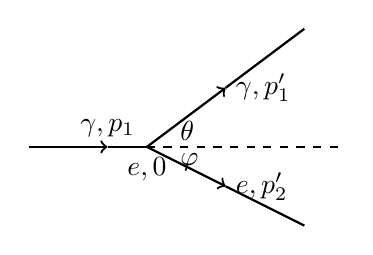
\begin{tikzpicture}
			\draw[->,thick](0,0)--(1,0)node[anchor=south]{$\gamma,p_1$};
			\draw[thick](1,0)--(1.5,0)node[anchor=north]{$e,0$};
			\draw[->,thick](1.5,0)--(2.5,0.75)node[anchor=west]{$\gamma,p_1'$};
			\draw[thick](2.5,0.75)--(3.5,1.5);
			\draw[->,thick](1.5,0)--(2.5,-0.5)node[anchor=west]{$e,p_2'$};
			\draw[thick](2.5,-0.5)--(3.5,-1);
			\draw[dashed,thick](1.5,0)--(4,0);
			\draw(1.8,0.2)node[anchor=west]{$\theta$};
			\draw(1.8,-0.2)node[anchor=west]{$\varphi$};
		\end{tikzpicture}
	\end{figure}
	由四动量守恒
	\begin{align*}
		p_1&=p_1'\cos\theta+p_2'\cos\varphi,\\
		0&=p_1'\sin\theta-p_2'\sin\varphi,\\
		p_1+m_ec&=p_1'+\sqrt{m_e^2c^2+p_2'^2},
	\end{align*}
	求解可以得到散射之后光子频率的变化
	\[\frac{\omega'}{\omega}=\frac{1}{1+\frac{\hbar\omega}{m_ec^2}(1-\cos\theta)}.\]
	
	\section{束缚电子对电磁波的散射}
	
	最简单的束缚模型之一是简谐势
	\[m\ddot{\b{r}}+m\omega_0^2\b{r}-m\tau\dddot{\b{r}}=-e\b{E}_0\e^{-\i\omega t},\]
	我们进行同样的近似得到(其中$\gamma=\omega^2\tau$)
	\[\ddot{\b{r}}+\omega^2_0\b{r}+\gamma\dot{\b{r}}=-\frac{e}{m}\b{E}_0\e^{-\i\omega t},\]
	它的解为
	\[\b{r}=\b{r}_0\e^{-\frac{\gamma t}{2}}\e^{-\i\omega_0 t}-\frac{e\b{E}_0}{m}\frac{1}{(\omega_0^2-\omega^2)-\i\omega\gamma}\e^{-\i\omega t},\]
	即为有阻尼的本征振动和外场驱动振动的叠加。考虑时间足够长,本征振动可以忽略,那么
	\begin{align*}
		\b{r}&=-\frac{e\b{E}_0}{m}\frac{1}{(\omega_0^2-\omega^2)-\i\omega\gamma}\e^{-\i\omega t}\\
		&=-\frac{e\b{E}_0}{m}\frac{1}{\sqrt{(\omega_0^2-\omega^2)^2+\omega^2\gamma^2}}\e^{-\i(\omega t+\delta)}\\
		&=\b{r}_0'\e^{-\i(\omega t+\delta)}
	\end{align*}
	可以看到,我们又得到了一个类似的电偶极矩,只是内部形式比以前复杂一些。可以推导出总辐射功率
	\[\overline{P}=\frac{1}{2}\frac{e^2a^2}{6\pi\varepsilon_0c^3}=\frac{e^4}{6\pi\varepsilon_0^2c^4m^2}\frac{\omega^4}{(\omega_0^2-\omega^2)^2+\omega^2\gamma^2}\left(\frac{1}{2}\varepsilon_0E_0^2c\right),\]
	最后一项即为入射波的能流密度,因而可以定义这一问题下的散射截面
	\[\sigma=\sigma_T\frac{\omega^4}{(\omega_0^2-\omega^2)^2+\omega^2\gamma^2},\]
	$\sigma_T$是先前求得的自由电子情况下的散射截面。
	
	讨论几种情况
	\begin{itemize}
		\item $\omega\ll \omega_0$
			
			此时
			\[\sigma=\sigma_T\left(\frac{\omega}{\omega_0}\right)^4,\]
			这即为瑞利散射公式,说明了天空显示蓝色的原因。
		\item $\omega \sim \omega_0$
		
			此时
			\[\sigma=\sigma_T\left(\frac{\omega}{\gamma}\right)^2,\]
			这是构成共振散射。
			
		\item $\omega\gg \omega_0$
		
		此时
		\[\sigma=\sigma_T,\]
		即过渡到汤姆孙散射情形。
	\end{itemize}
	
	\section{介质对电磁波的吸收和色散}
	
	\subsection{介质的介电常数}
	我们假设介质由大量的($N$个)经典振子组成,这些振子只有一个振动频率$\omega_0$,由我们在上一节的讨论,极化强度可以写为
	\[\b{P}=-Ne\b{r}=\frac{Ne^2}{m}\frac{1}{(\omega_0^2-\omega^2)-\i\omega\gamma}\b{E}=\mathcal{X}_e\varepsilon_0\b{E},\]
	介电常数
	\[\varepsilon=\varepsilon_0+\varepsilon_0\mathcal{X}_e=\varepsilon_0+\frac{Ne^2}{m}\frac{1}{(\omega_0^2-\omega^2)-\i\omega\gamma}.\]
	
	考虑在介质中沿$z$中传播的平面电磁波
	\[\b{E}=\b{E}_0\e^{\i(kz-\omega t)},\]
	那么由波动方程可以解出色散关系
	\[k=\frac{1}{c}n\omega=\frac{1}{c}\sqrt{\frac{\varepsilon}{\varepsilon_0}}\omega.\]
	注意到介质中介电常数为负数,因此波矢也是复数,不妨将其写为
	\[k=b+\i a,\quad a,b\in \mathcal{R},\]
	那么
	\[\b{E}=\b{E}_0\e^{-az}\e^{\i(bz-\omega t)},\]
	可见,波矢的虚部导致电磁波在介质中的衰减。下面来求实部和虚部的具体形式。将折射率写成实部和虚部(已经近似过了)
	\[n_r=1+\frac{Ne^2}{2m\varepsilon_0}\frac{\omega_0^2-\omega^2}{(\omega_0^2-\omega^2)^2+\omega^2\gamma^2},\quad n_i=\frac{N e^2}{2m\varepsilon_0}\frac{\omega \gamma}{(\omega_0^2-\omega^2)^2+\omega^2\gamma^2},\]
	而
	\[b=\frac{n_r\omega}{c},\quad a=\frac{n_i\omega}{c}.\]
	
	\subsection{介质对电磁波的吸收}
	
	我们可以看到,介质中的表达式与导体中的表达式具有一定的相似性,但二者背后的物理是不同的。导体中电磁波损失的能量转化为电子的振动能量,而介质中电磁波损失的能量被振子以辐射的方式损失掉。
	
	\subsection{介质的色散}
	
	我们知道相速度
	\[v=\frac{\omega}{k_r}=\frac{\omega }{b}=\frac{c}{n_r},\]
	因而相速度是与频率相关的。这说明对于不同波长的电磁波组成的波包,它在传播过程中会发生色散。	
	
	设单位体积内有$N$个原子,每个原子有$Z$个电子,固有频率为$\omega_j$的振子数量为$f_j$,阻尼常数$\gamma_j$,那么介电常数可以推广为
	\[\varepsilon_r(\omega)=1+\frac{Ne^2}{m\varepsilon_0}\sum_j\frac{f_j}{(\omega_j^2-\omega^2)-\i\omega\gamma_j},\]
	从而我们可以推导出其他公式的推广形式。
	
	
	
	
	
	
	
	
	
	
	
	
	
\end{document}